% Options for packages loaded elsewhere
\PassOptionsToPackage{unicode}{hyperref}
\PassOptionsToPackage{hyphens}{url}
\PassOptionsToPackage{dvipsnames,svgnames,x11names}{xcolor}
%
\documentclass[
  letterpaper,
  DIV=11,
  numbers=noendperiod]{scrartcl}

\usepackage{amsmath,amssymb}
\usepackage{iftex}
\ifPDFTeX
  \usepackage[T1]{fontenc}
  \usepackage[utf8]{inputenc}
  \usepackage{textcomp} % provide euro and other symbols
\else % if luatex or xetex
  \usepackage{unicode-math}
  \defaultfontfeatures{Scale=MatchLowercase}
  \defaultfontfeatures[\rmfamily]{Ligatures=TeX,Scale=1}
\fi
\usepackage{lmodern}
\ifPDFTeX\else  
    % xetex/luatex font selection
\fi
% Use upquote if available, for straight quotes in verbatim environments
\IfFileExists{upquote.sty}{\usepackage{upquote}}{}
\IfFileExists{microtype.sty}{% use microtype if available
  \usepackage[]{microtype}
  \UseMicrotypeSet[protrusion]{basicmath} % disable protrusion for tt fonts
}{}
\makeatletter
\@ifundefined{KOMAClassName}{% if non-KOMA class
  \IfFileExists{parskip.sty}{%
    \usepackage{parskip}
  }{% else
    \setlength{\parindent}{0pt}
    \setlength{\parskip}{6pt plus 2pt minus 1pt}}
}{% if KOMA class
  \KOMAoptions{parskip=half}}
\makeatother
\usepackage{xcolor}
\setlength{\emergencystretch}{3em} % prevent overfull lines
\setcounter{secnumdepth}{-\maxdimen} % remove section numbering
% Make \paragraph and \subparagraph free-standing
\ifx\paragraph\undefined\else
  \let\oldparagraph\paragraph
  \renewcommand{\paragraph}[1]{\oldparagraph{#1}\mbox{}}
\fi
\ifx\subparagraph\undefined\else
  \let\oldsubparagraph\subparagraph
  \renewcommand{\subparagraph}[1]{\oldsubparagraph{#1}\mbox{}}
\fi


\providecommand{\tightlist}{%
  \setlength{\itemsep}{0pt}\setlength{\parskip}{0pt}}\usepackage{longtable,booktabs,array}
\usepackage{calc} % for calculating minipage widths
% Correct order of tables after \paragraph or \subparagraph
\usepackage{etoolbox}
\makeatletter
\patchcmd\longtable{\par}{\if@noskipsec\mbox{}\fi\par}{}{}
\makeatother
% Allow footnotes in longtable head/foot
\IfFileExists{footnotehyper.sty}{\usepackage{footnotehyper}}{\usepackage{footnote}}
\makesavenoteenv{longtable}
\usepackage{graphicx}
\makeatletter
\def\maxwidth{\ifdim\Gin@nat@width>\linewidth\linewidth\else\Gin@nat@width\fi}
\def\maxheight{\ifdim\Gin@nat@height>\textheight\textheight\else\Gin@nat@height\fi}
\makeatother
% Scale images if necessary, so that they will not overflow the page
% margins by default, and it is still possible to overwrite the defaults
% using explicit options in \includegraphics[width, height, ...]{}
\setkeys{Gin}{width=\maxwidth,height=\maxheight,keepaspectratio}
% Set default figure placement to htbp
\makeatletter
\def\fps@figure{htbp}
\makeatother

\KOMAoption{captions}{tableheading}
\makeatletter
\makeatother
\makeatletter
\makeatother
\makeatletter
\@ifpackageloaded{caption}{}{\usepackage{caption}}
\AtBeginDocument{%
\ifdefined\contentsname
  \renewcommand*\contentsname{Table of contents}
\else
  \newcommand\contentsname{Table of contents}
\fi
\ifdefined\listfigurename
  \renewcommand*\listfigurename{List of Figures}
\else
  \newcommand\listfigurename{List of Figures}
\fi
\ifdefined\listtablename
  \renewcommand*\listtablename{List of Tables}
\else
  \newcommand\listtablename{List of Tables}
\fi
\ifdefined\figurename
  \renewcommand*\figurename{Figure}
\else
  \newcommand\figurename{Figure}
\fi
\ifdefined\tablename
  \renewcommand*\tablename{Table}
\else
  \newcommand\tablename{Table}
\fi
}
\@ifpackageloaded{float}{}{\usepackage{float}}
\floatstyle{ruled}
\@ifundefined{c@chapter}{\newfloat{codelisting}{h}{lop}}{\newfloat{codelisting}{h}{lop}[chapter]}
\floatname{codelisting}{Listing}
\newcommand*\listoflistings{\listof{codelisting}{List of Listings}}
\makeatother
\makeatletter
\@ifpackageloaded{caption}{}{\usepackage{caption}}
\@ifpackageloaded{subcaption}{}{\usepackage{subcaption}}
\makeatother
\makeatletter
\@ifpackageloaded{tcolorbox}{}{\usepackage[skins,breakable]{tcolorbox}}
\makeatother
\makeatletter
\@ifundefined{shadecolor}{\definecolor{shadecolor}{rgb}{.97, .97, .97}}
\makeatother
\makeatletter
\makeatother
\makeatletter
\makeatother
\ifLuaTeX
  \usepackage{selnolig}  % disable illegal ligatures
\fi
\IfFileExists{bookmark.sty}{\usepackage{bookmark}}{\usepackage{hyperref}}
\IfFileExists{xurl.sty}{\usepackage{xurl}}{} % add URL line breaks if available
\urlstyle{same} % disable monospaced font for URLs
\hypersetup{
  pdftitle={Kwantitatieve gegevensverwerking met Jamovi},
  pdfauthor={dr. Willem De Keyzer},
  colorlinks=true,
  linkcolor={blue},
  filecolor={Maroon},
  citecolor={Blue},
  urlcolor={Blue},
  pdfcreator={LaTeX via pandoc}}

\title{Kwantitatieve gegevensverwerking met Jamovi}
\usepackage{etoolbox}
\makeatletter
\providecommand{\subtitle}[1]{% add subtitle to \maketitle
  \apptocmd{\@title}{\par {\large #1 \par}}{}{}
}
\makeatother
\subtitle{Onderzoeksskills 2}
\author{dr. Willem De Keyzer}
\date{2023}

\begin{document}
\maketitle
\begin{abstract}
Aan het einde van deze modele zul je de volgende tools en functies van
Jamovi kennen:

\begin{itemize}
\tightlist
\item
  Navigeren door en gebruikmaken van de Jamovi-omgeving
\item
  Variabelen en cases verkennen en maken
\item
  Beschrijvende gegevensverwerking
\item
  Eenvoudige grafieken en boxplots
\item
  Parametrisch testen
\end{itemize}

\begin{tcolorbox}[beforeafter skip=1cm, ignore nobreak=true, breakable, colframe=Questions-frame, colback=Questions-bg, coltext=Questions-text, boxsep=2mm, arc=0mm, boxrule=0.5mm]

Doorheen de module zijn er \textbf{leercontroles} (genummerd Q1, Q2,
enz.) die je vragen stellen over wat er zojuist is behandeld. Deze
vragen worden niet gesteld ter beoordeling, maar om je te helpen Jamovi
volledig te leren gebruiken. De antwoorden op alle vragen staan aan het
einde van deze module zodat je kunt controleren of je het goed hebt
gedaan en je kunt op de vraagnummers klikken om naar dat antwoord te
gaan.

\end{tcolorbox}
\end{abstract}
\ifdefined\Shaded\renewenvironment{Shaded}{\begin{tcolorbox}[breakable, frame hidden, interior hidden, enhanced, borderline west={3pt}{0pt}{shadecolor}, sharp corners, boxrule=0pt]}{\end{tcolorbox}}\fi

\hypertarget{vertrouwd-raken-met-jamovi}{%
\section{Vertrouwd raken met Jamovi}\label{vertrouwd-raken-met-jamovi}}

In dit gedeelte zullen we vooral wennen aan het gebruik van Jamovi en
het instellen van onze gegevens.

\hypertarget{jamovi-op-je-eigen-computer-installeren}{%
\subsection{Jamovi op je eigen computer
installeren}\label{jamovi-op-je-eigen-computer-installeren}}

Omdat Jamovi een gratis en open-source applicatie is, kan je deze
eenvoudig op je eigen computer installeren. Download het
Jamovi-installatieprogramma voor jouw systeem van:

\url{https://www.jamovi.org/download.html}

Als je de optie krijgt, kies dan de versie `\textbf{Solid}'. Zodra het
installatieprogramma is gedownload, dubbelklik je erop om Jamovi op je
computer te installeren. Voor een volledige handleiding en instructies
voor het installeren van Jamovi, zie sectie 1 van de
\textbf{Jamovi-gebruikershandleiding} hier:

\url{https://www.jamovi.org/user-manual.html}

Jamovi is een gewone applicatie-installatie voor Windows en Mac, maar
Jamovi is ook beschikbaar voor Linux en Chromebooks met enkele extra
stappen (zie de bovenstaande gebruikershandleiding voor meer
informatie). Als je Jamovi om de een of andere reden niet op je computer
kunt installeren, kun je hier een online versie van Jamovi gebruiken:

\url{https://cloud.jamovi.org/}

\begin{tcolorbox}[beforeafter skip=1cm, ignore nobreak=true, breakable, colframe=Aside-frame, colback=Aside-bg, coltext=Aside-text, boxsep=2mm, arc=0mm, boxrule=0.5mm]

Houd er rekening mee dat de online versie van Jamovi slechts een
demoversie is en niet altijd beschikbaar is. Het wordt \textbf{sterk
aanbevolen} om Jamovi op je eigen computer te installeren als dat
mogelijk is.

\end{tcolorbox}

\hypertarget{hulp-met-jamovi}{%
\subsection{Hulp met Jamovi}\label{hulp-met-jamovi}}

Jamovi heeft veel online hulpbronnen om je te helpen bij het gebruik!
Naast de gebruikershandleiding waarnaar hierboven wordt verwezen, kan je
hier een aantal nuttige gidsen vinden op de pagina met hulpmiddelen van
de Jamovi-gemeenschap:

\url{https://www.jamovi.org/community.html}

Er is met name een YouTube-afspeellijst met nuttige Jamovi-videogidsen
(\href{https://bit.ly/jamovi-youtube}{klik hier}) en een volledig
handboek over statistiek met Jamovi
(\href{https://www.learnstatswithjamovi.com/}{klik hier}) gelinkt aan de
pagina met hulpmiddelen van de community die handig kunnen zijn als je
hulp nodig hebt buiten een tutorial om, of als je nog meer details wilt
weten over statistiek met Jamovi.

\hypertarget{download-de-gegevensbestanden}{%
\subsection{Download de
gegevensbestanden}\label{download-de-gegevensbestanden}}

Download \textbf{alle} Jamovi-gegevensbestanden van
\href{https://github.com/wdkeyzer/jamovi-worksheets/tree/master/00-Data-Files}{GitHub}
en sla ze ergens op waar je er gemakkelijk bij kunt.

Jamovi gebruikt de `.omv' bestandsextensie, wat een aangepast
bestandsformaat is. In tegenstelling tot andere bestandsformaten kun je
deze niet dubbelklikken als snelkoppeling om ze in Jamovi te openen -
maak je geen zorgen, je moet gewoon eerst Jamovi openen en ze dan vanuit
Jamovi openen.

\hypertarget{eerste-kennismaking-met-jamovi}{%
\subsection{Eerste kennismaking met
Jamovi}\label{eerste-kennismaking-met-jamovi}}

Open na de installatie de Jamovi-toepassing. Je zou een lege
Jamovi-werkruimte moeten zien:

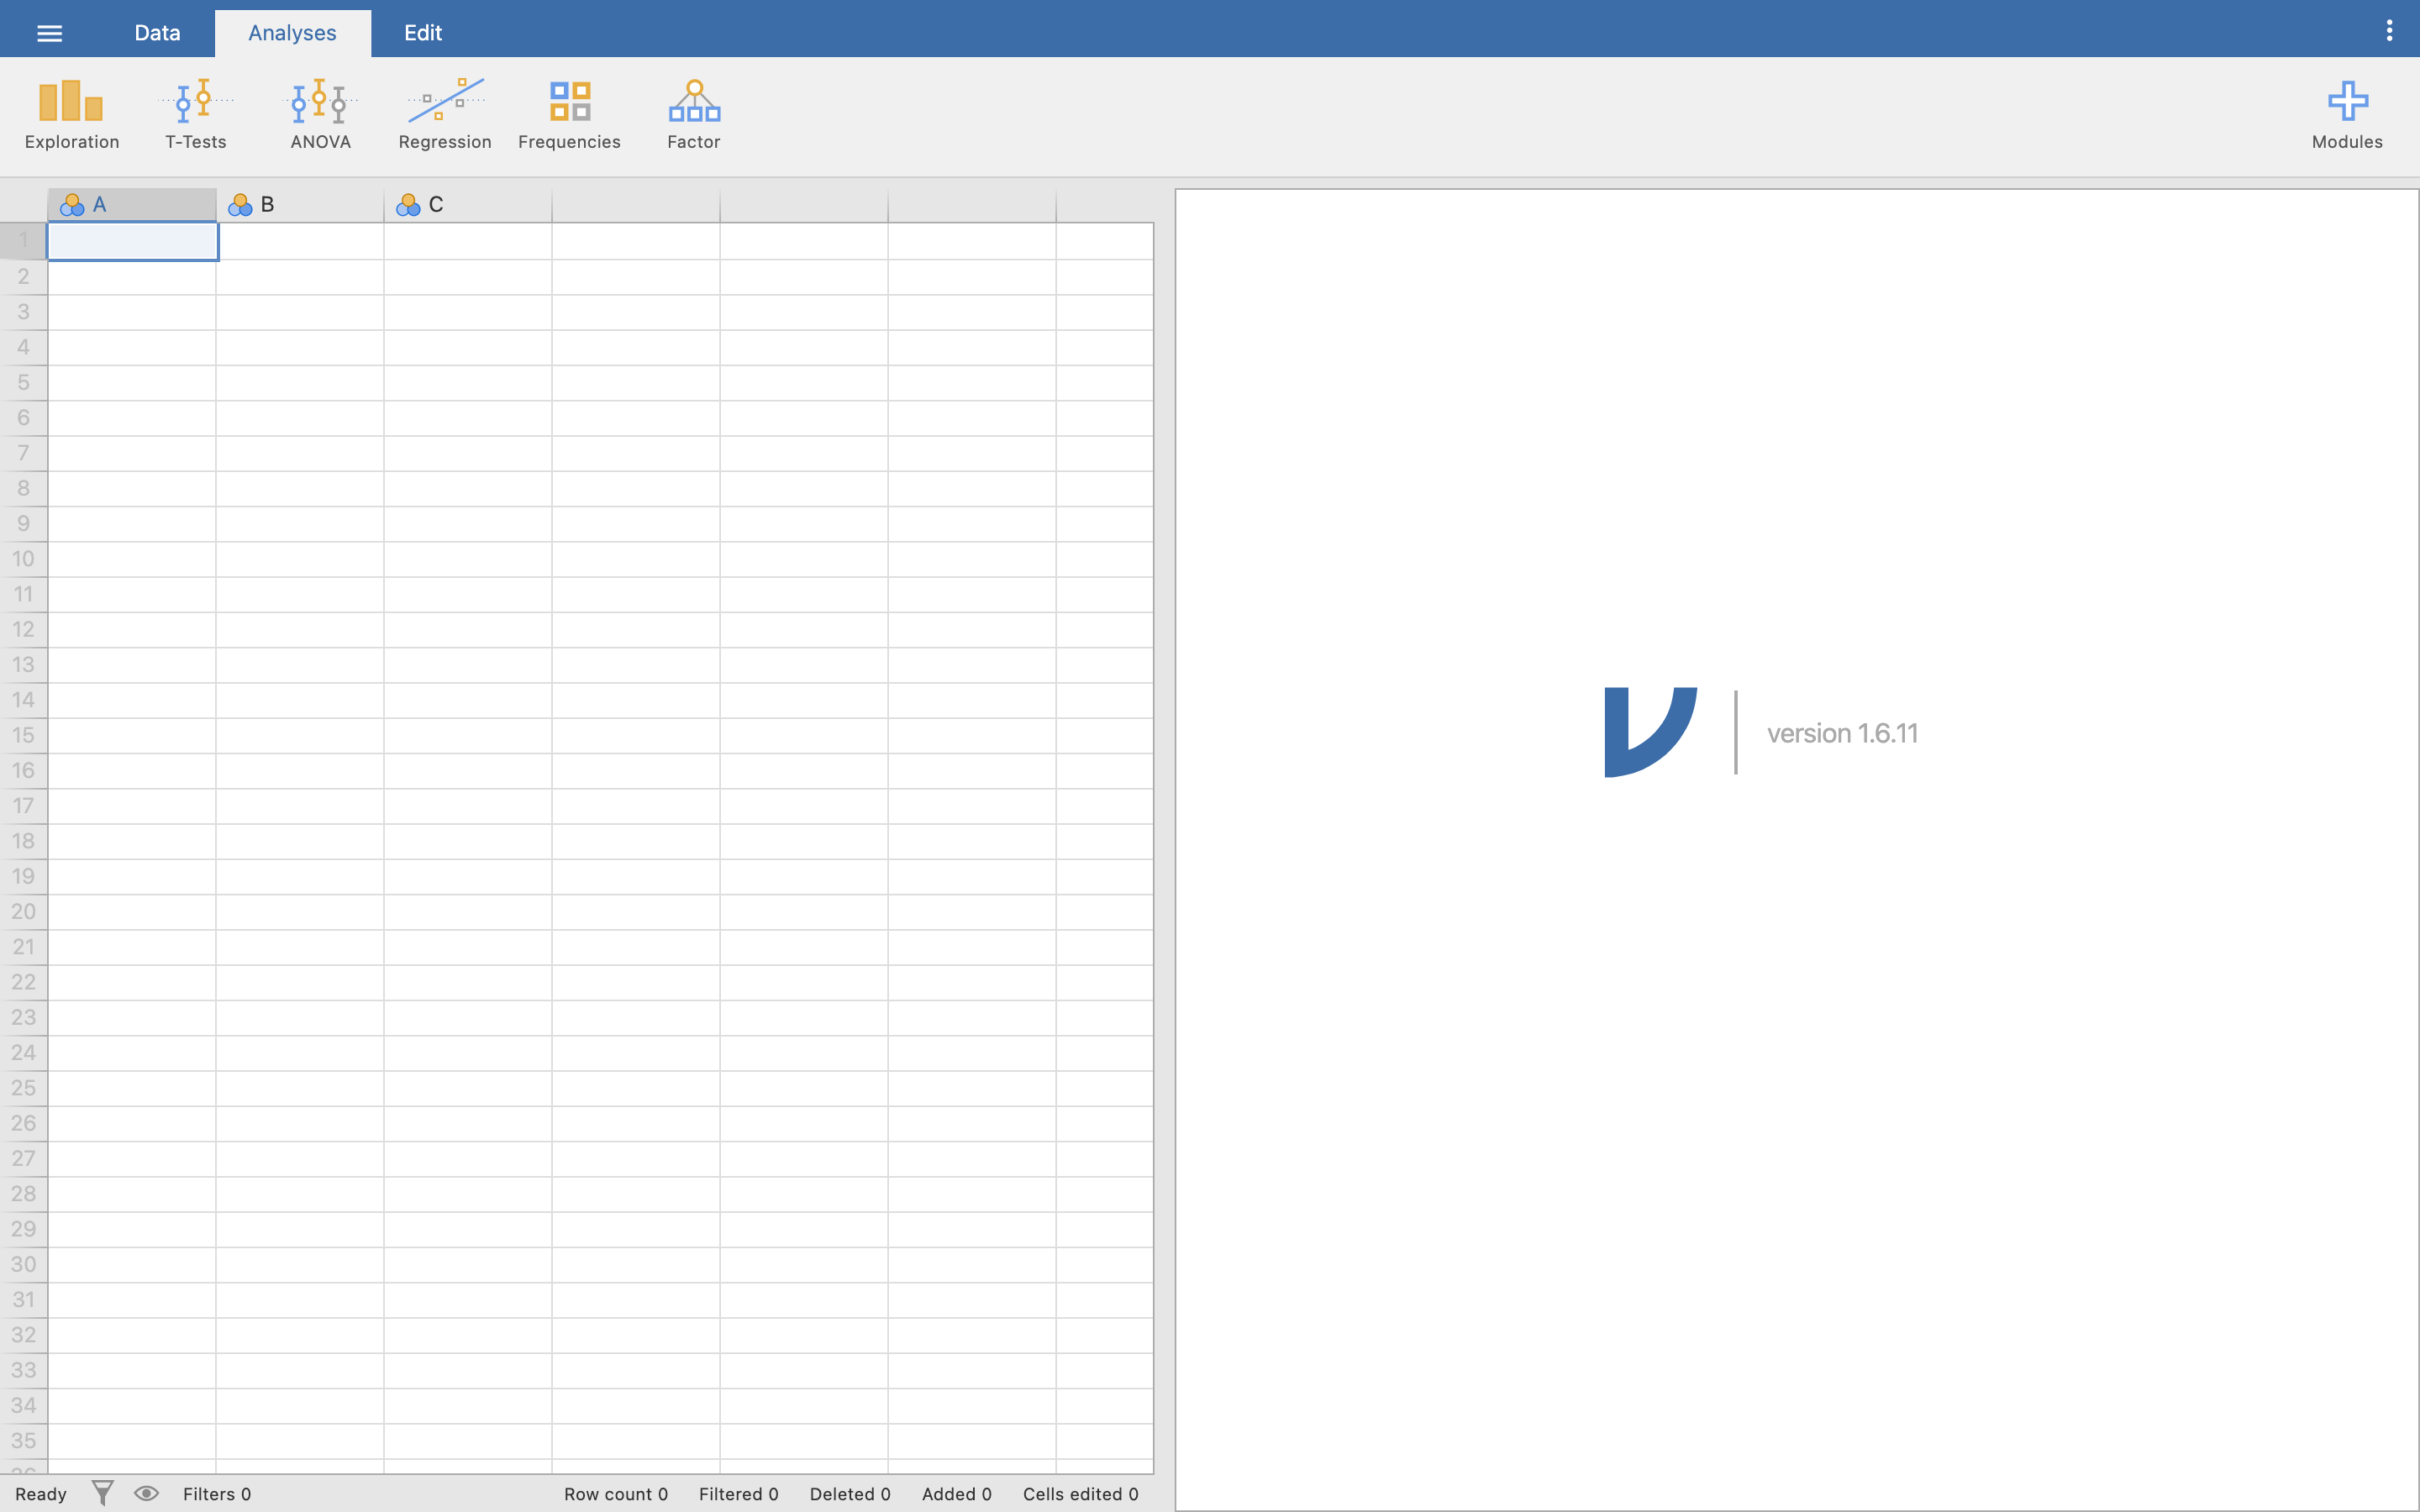
\includegraphics{_imgs/01-01.png}

De werkruimte in Jamovi is verdeeld in een aantal secties.

\begin{itemize}
\tightlist
\item
  Het grote rasterachtige gebied aan de linkerkant (dat eruit ziet als
  Excel) is het \textbf{Spreadsheet}. Hier komen je gegevens te staan!
\item
  Het lege gebied aan de rechterkant is de \textbf{Results Viewer}. Dit
  is een blanco vel papier waarop Jamovi de resultaten afdrukt van alle
  tests die je uitvoert. Je zult binnenkort zien hoe dit werkt.
\item
  Bovenaan staat het \textbf{Menu}. Dit heeft een paar opties -
  \textbf{Data}, \textbf{Analyses} en \textbf{Edit}. We zullen vooral
  Data en Analyses gebruiken. Als je op een van deze opties klikt,
  verandert het \textbf{lint} direct eronder om te laten zien wat je met
  elke optie kunt doen - in de schermafbeelding hierboven hebben we
  \textbf{Analyses} geselecteerd, dus het lint toont ons alle
  verschillende Analysetests die we kunnen uitvoeren.
\end{itemize}

Het menu heeft ook drie gestapelde witte lijnen in de linkerhoek - dit
opent het \textbf{File} menu. Klik daar nu op, klik dan op
\textbf{Open}, vervolgens op \textbf{Browse} en navigeer naar de plaats
waar je alle gegevensbestanden van hebt opgeslagen:

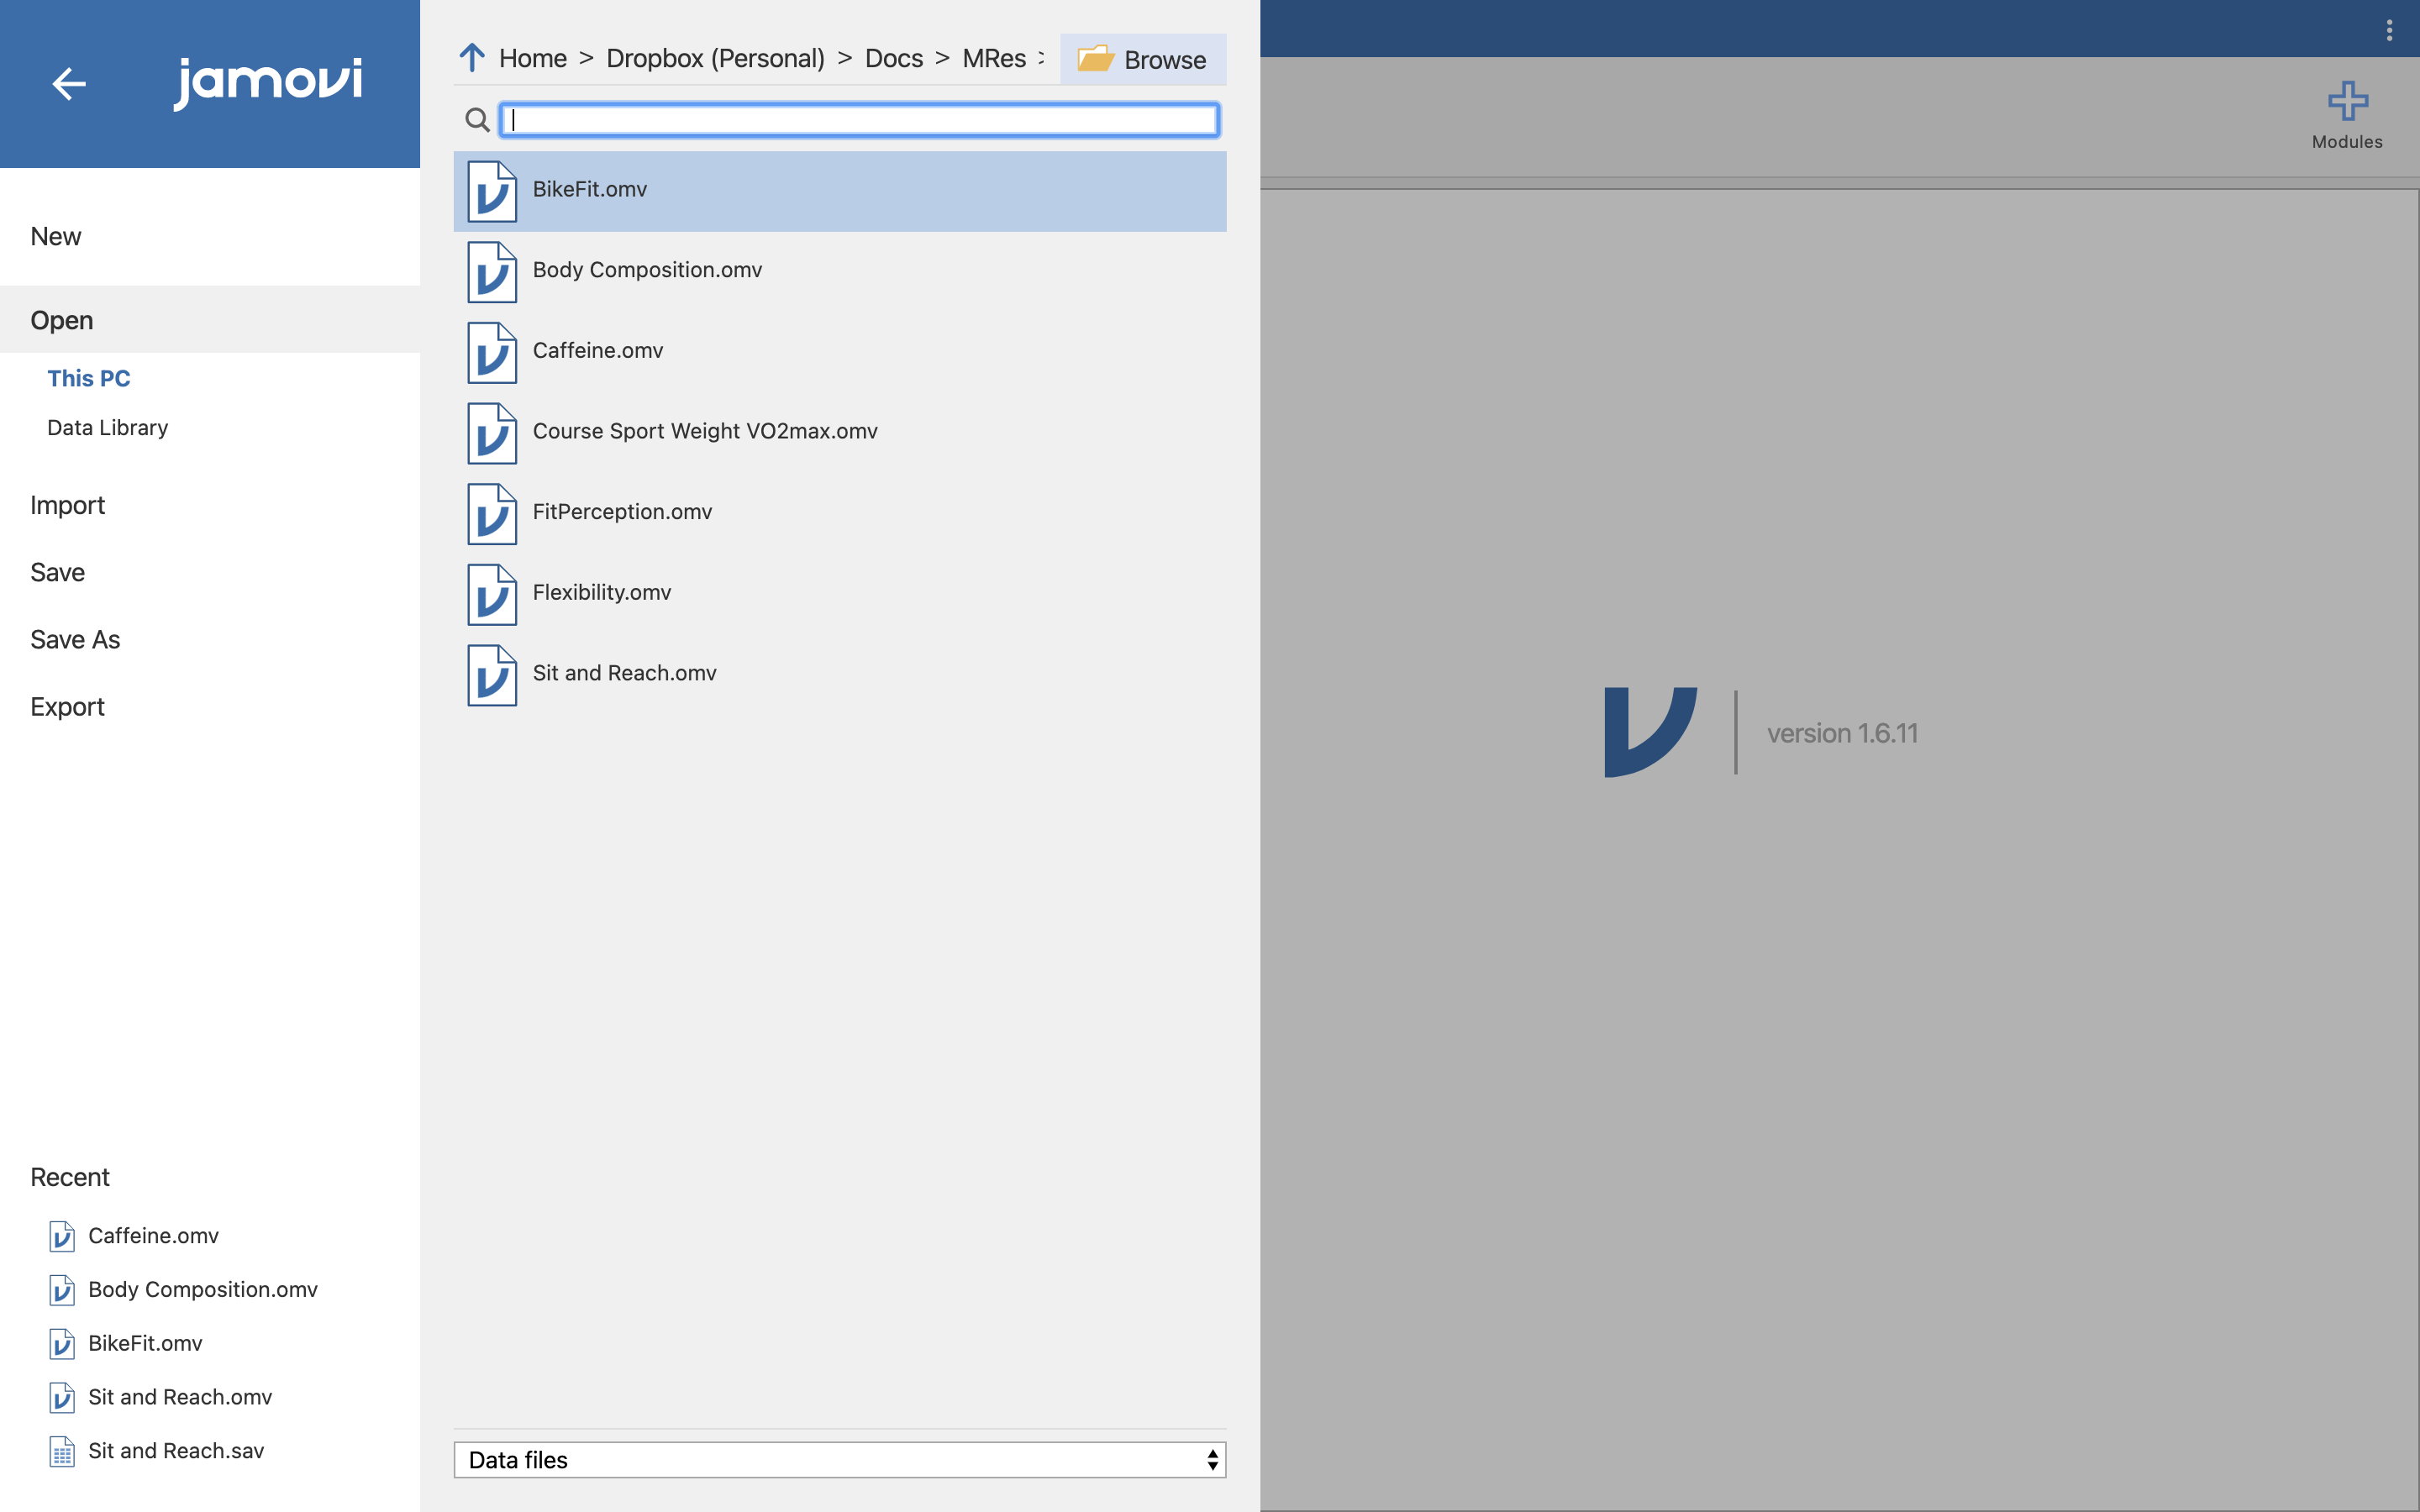
\includegraphics{_imgs/01-02.png}

Open het bestand \textbf{Body Composition.omv}.

Je zou nu gegevens moeten zien in de Spreadsheet-weergave. Als je meer
gegevens wilt zien, kan je de grootte van de Spreadsheet en Results
Viewer aanpassen door de dikke grijze lijn in het midden van het scherm
aan te klikken en te verslepen.

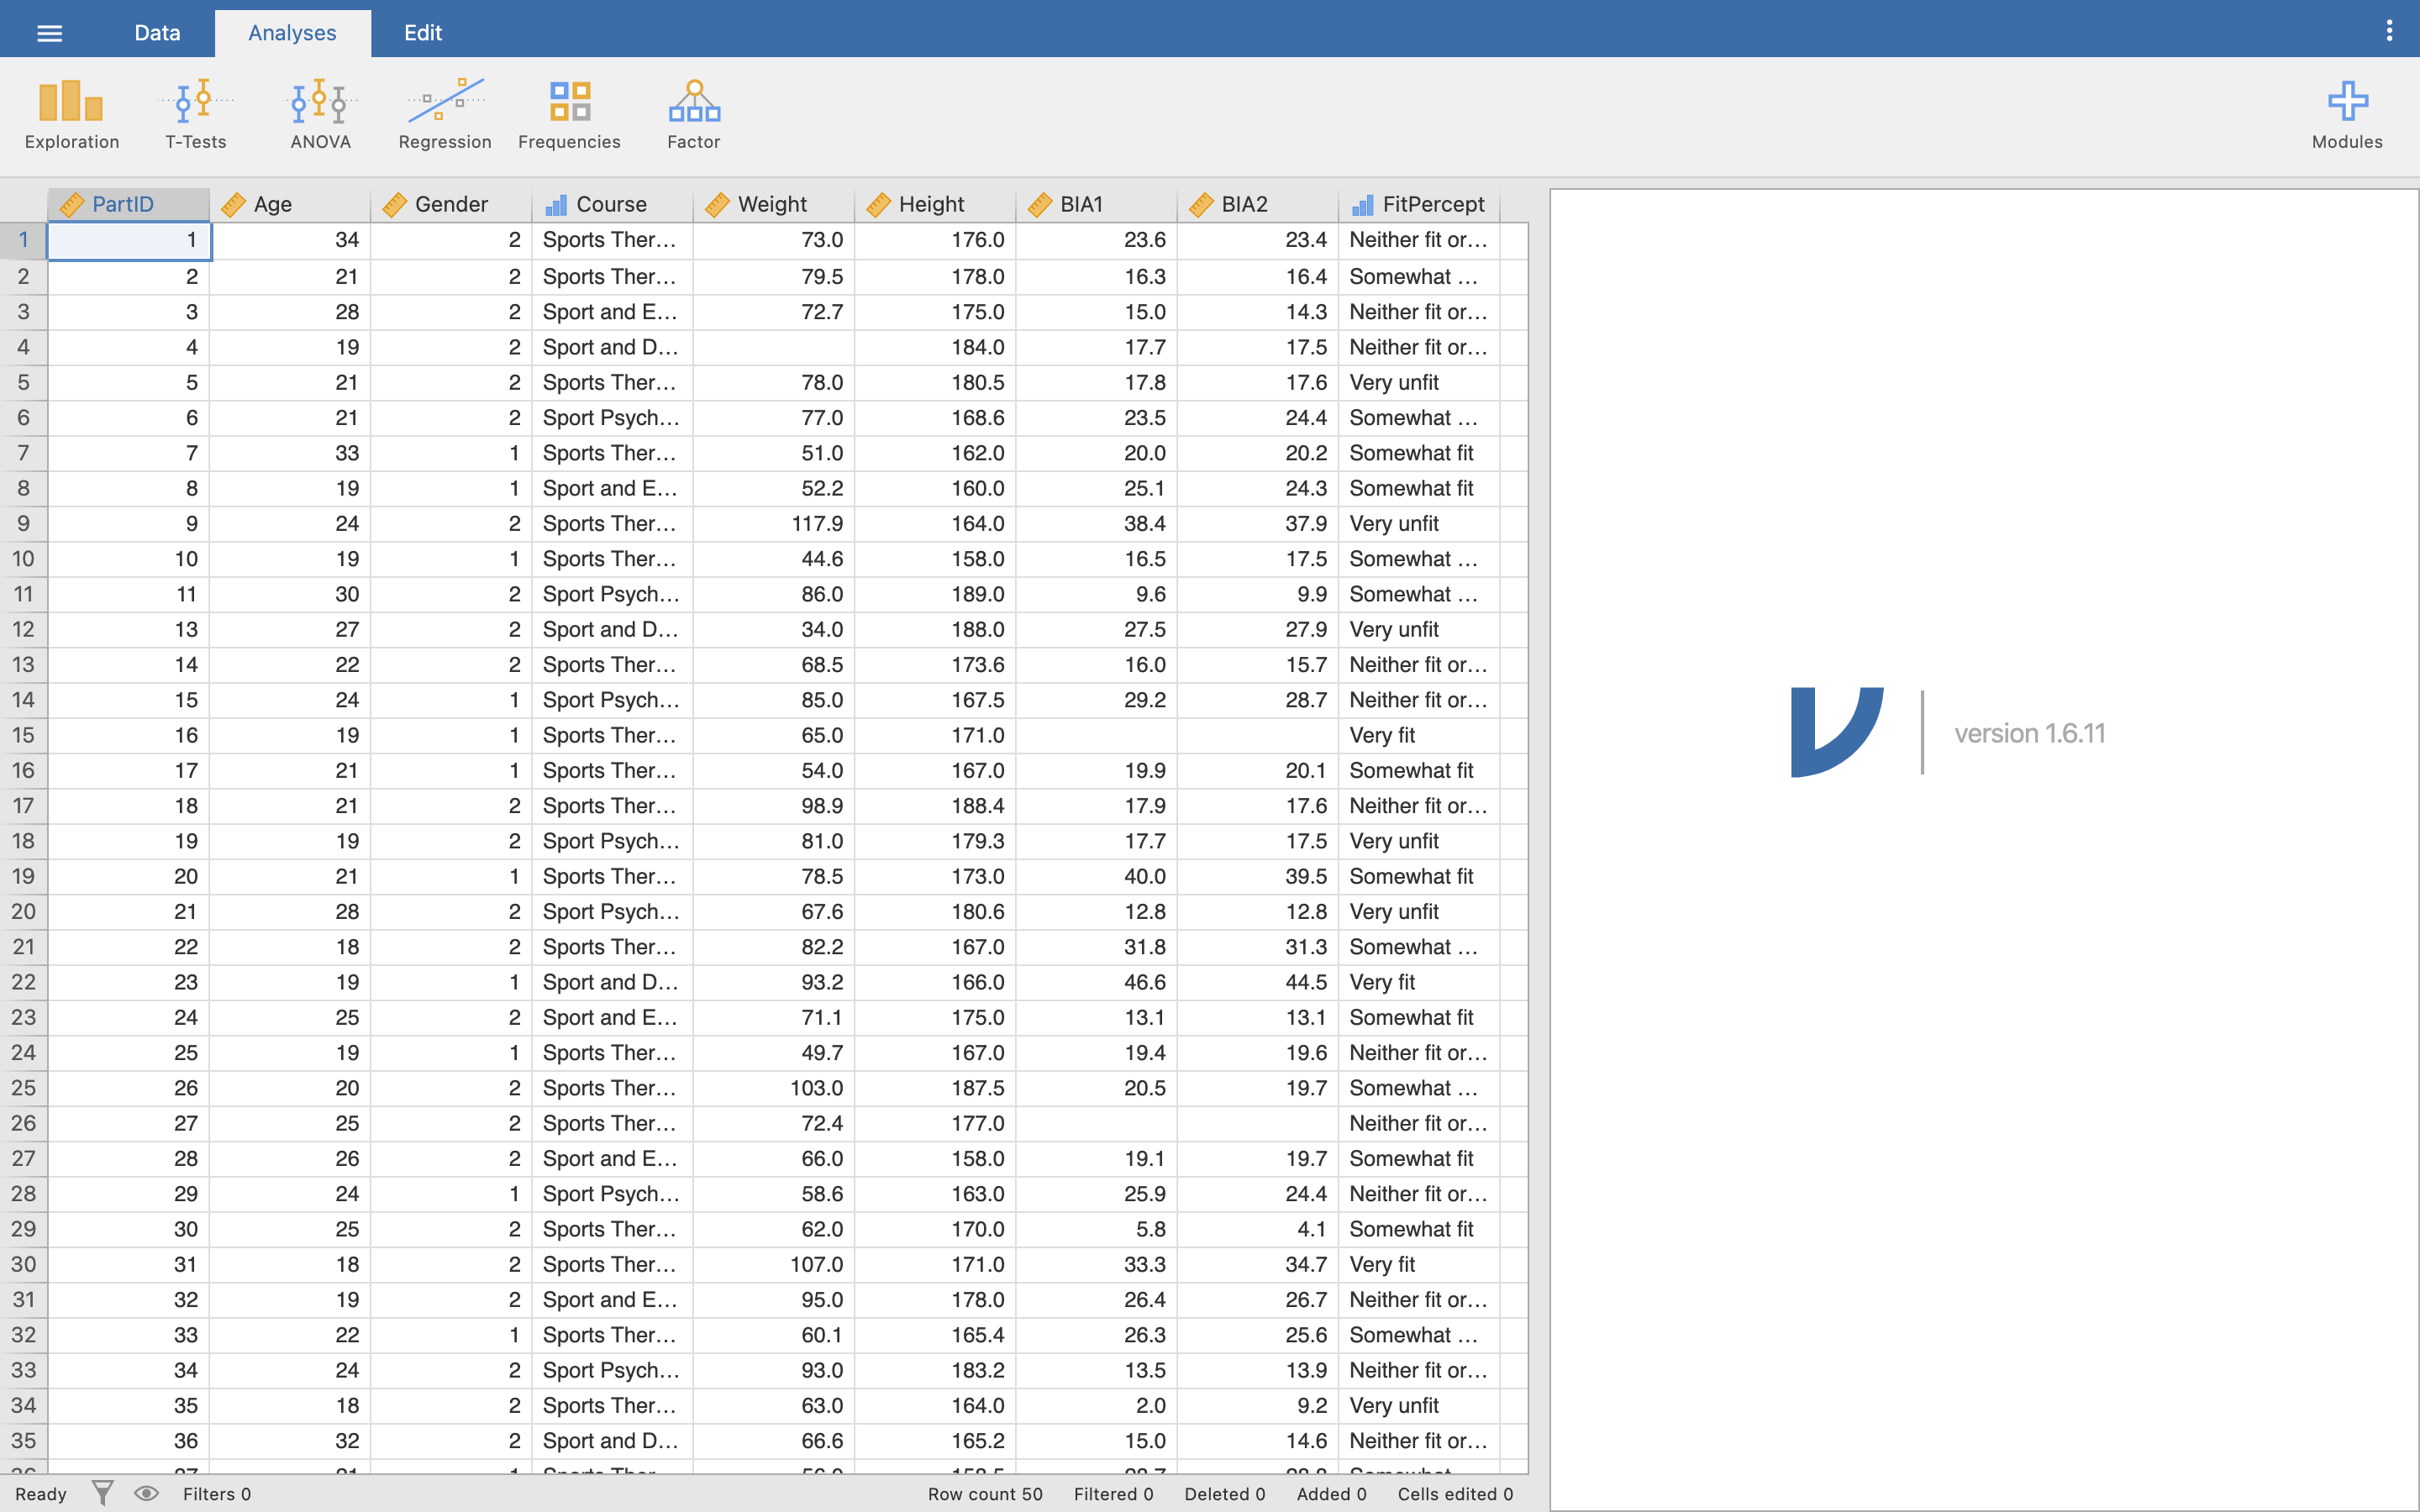
\includegraphics{_imgs/01-03.png}

\hypertarget{cases-en-variabelen}{%
\subsection{Cases en variabelen}\label{cases-en-variabelen}}

In Jamovi staat elke \textbf{kolom} voor een \textbf{variabele}, net als
in Excel, en elke \textbf{rij} voor een \textbf{case} (eenheid). Vergeet
niet om persoonlijke gegevens minstens te pseudonimiseren door een
anoniem nummer te gebruiken. In dit bestand wordt deze variabele
`PartID' genoemd.

\begin{tcolorbox}[beforeafter skip=1cm, ignore nobreak=true, breakable, colframe=Questions-frame, colback=Questions-bg, coltext=Questions-text, boxsep=2mm, arc=0mm, boxrule=0.5mm]

\protect\hypertarget{Q1}{\protect\hyperlink{A1}{Q1}}. Hoeveel kolommen
met gegevens zijn er?

\protect\hypertarget{Q2}{\protect\hyperlink{A2}{Q2}}. Hoeveel rijen
gegevens zijn er?

\protect\hypertarget{Q3}{\protect\hyperlink{A3}{Q3}}. Waarom een
deelnemers-ID als er een recordnummer is?

\protect\hypertarget{Q4}{\protect\hyperlink{A4}{Q4}}. Waarom hebben we
hoe dan ook een deelnemers-ID nodig? Waarom gebruiken we niet gewoon de
naam van de deelnemer?

\end{tcolorbox}

Bekijk de kolom PartID - merk op dat sommige ID's ontbreken, zodat het
rijnummer niet altijd overeenkomt met het nummer Participant ID
(PartID).

Voeg nog een eenheid toe aan de gegevens, typ de volgende nummers
onderaan het blad. Je kunt rechtstreeks in elke cel typen (vergelijkbaar
met Excel).

\begin{itemize}
\tightlist
\item
  PartID: 53
\item
  Age: 21
\item
  Gender: 2
\item
  Course: {[}laat leeg{]}
\item
  Weight: 41.0
\item
  Height: 160.0
\item
  BIA1: 18.8
\item
  BIA2: 18.8
\item
  FitPercept: {[}laat leeg{]}
\end{itemize}

\hypertarget{variabelen-instellen}{%
\subsubsection{Variabelen instellen}\label{variabelen-instellen}}

Tot nu toe gedraagt het gegevensblad zich ongeveer zoals Excel wat
betreft wat we kunnen invoeren. Maar in tegenstelling tot Excel kunnen
we in Jamovi meer informatie invoeren over wat er in elk van onze
variabelen (de kolommen in het gegevensblad) staat. Dit staat bekend als
\textbf{metadata}. Om deze te bewerken, klik je op \textbf{Data} en
vervolgens op \textbf{Setup} (het pictogram dat eruitziet als een
tandwiel bovenop een mini gegevensblad). Er wordt een extra menu geopend
bovenaan het Jamovi-scherm:

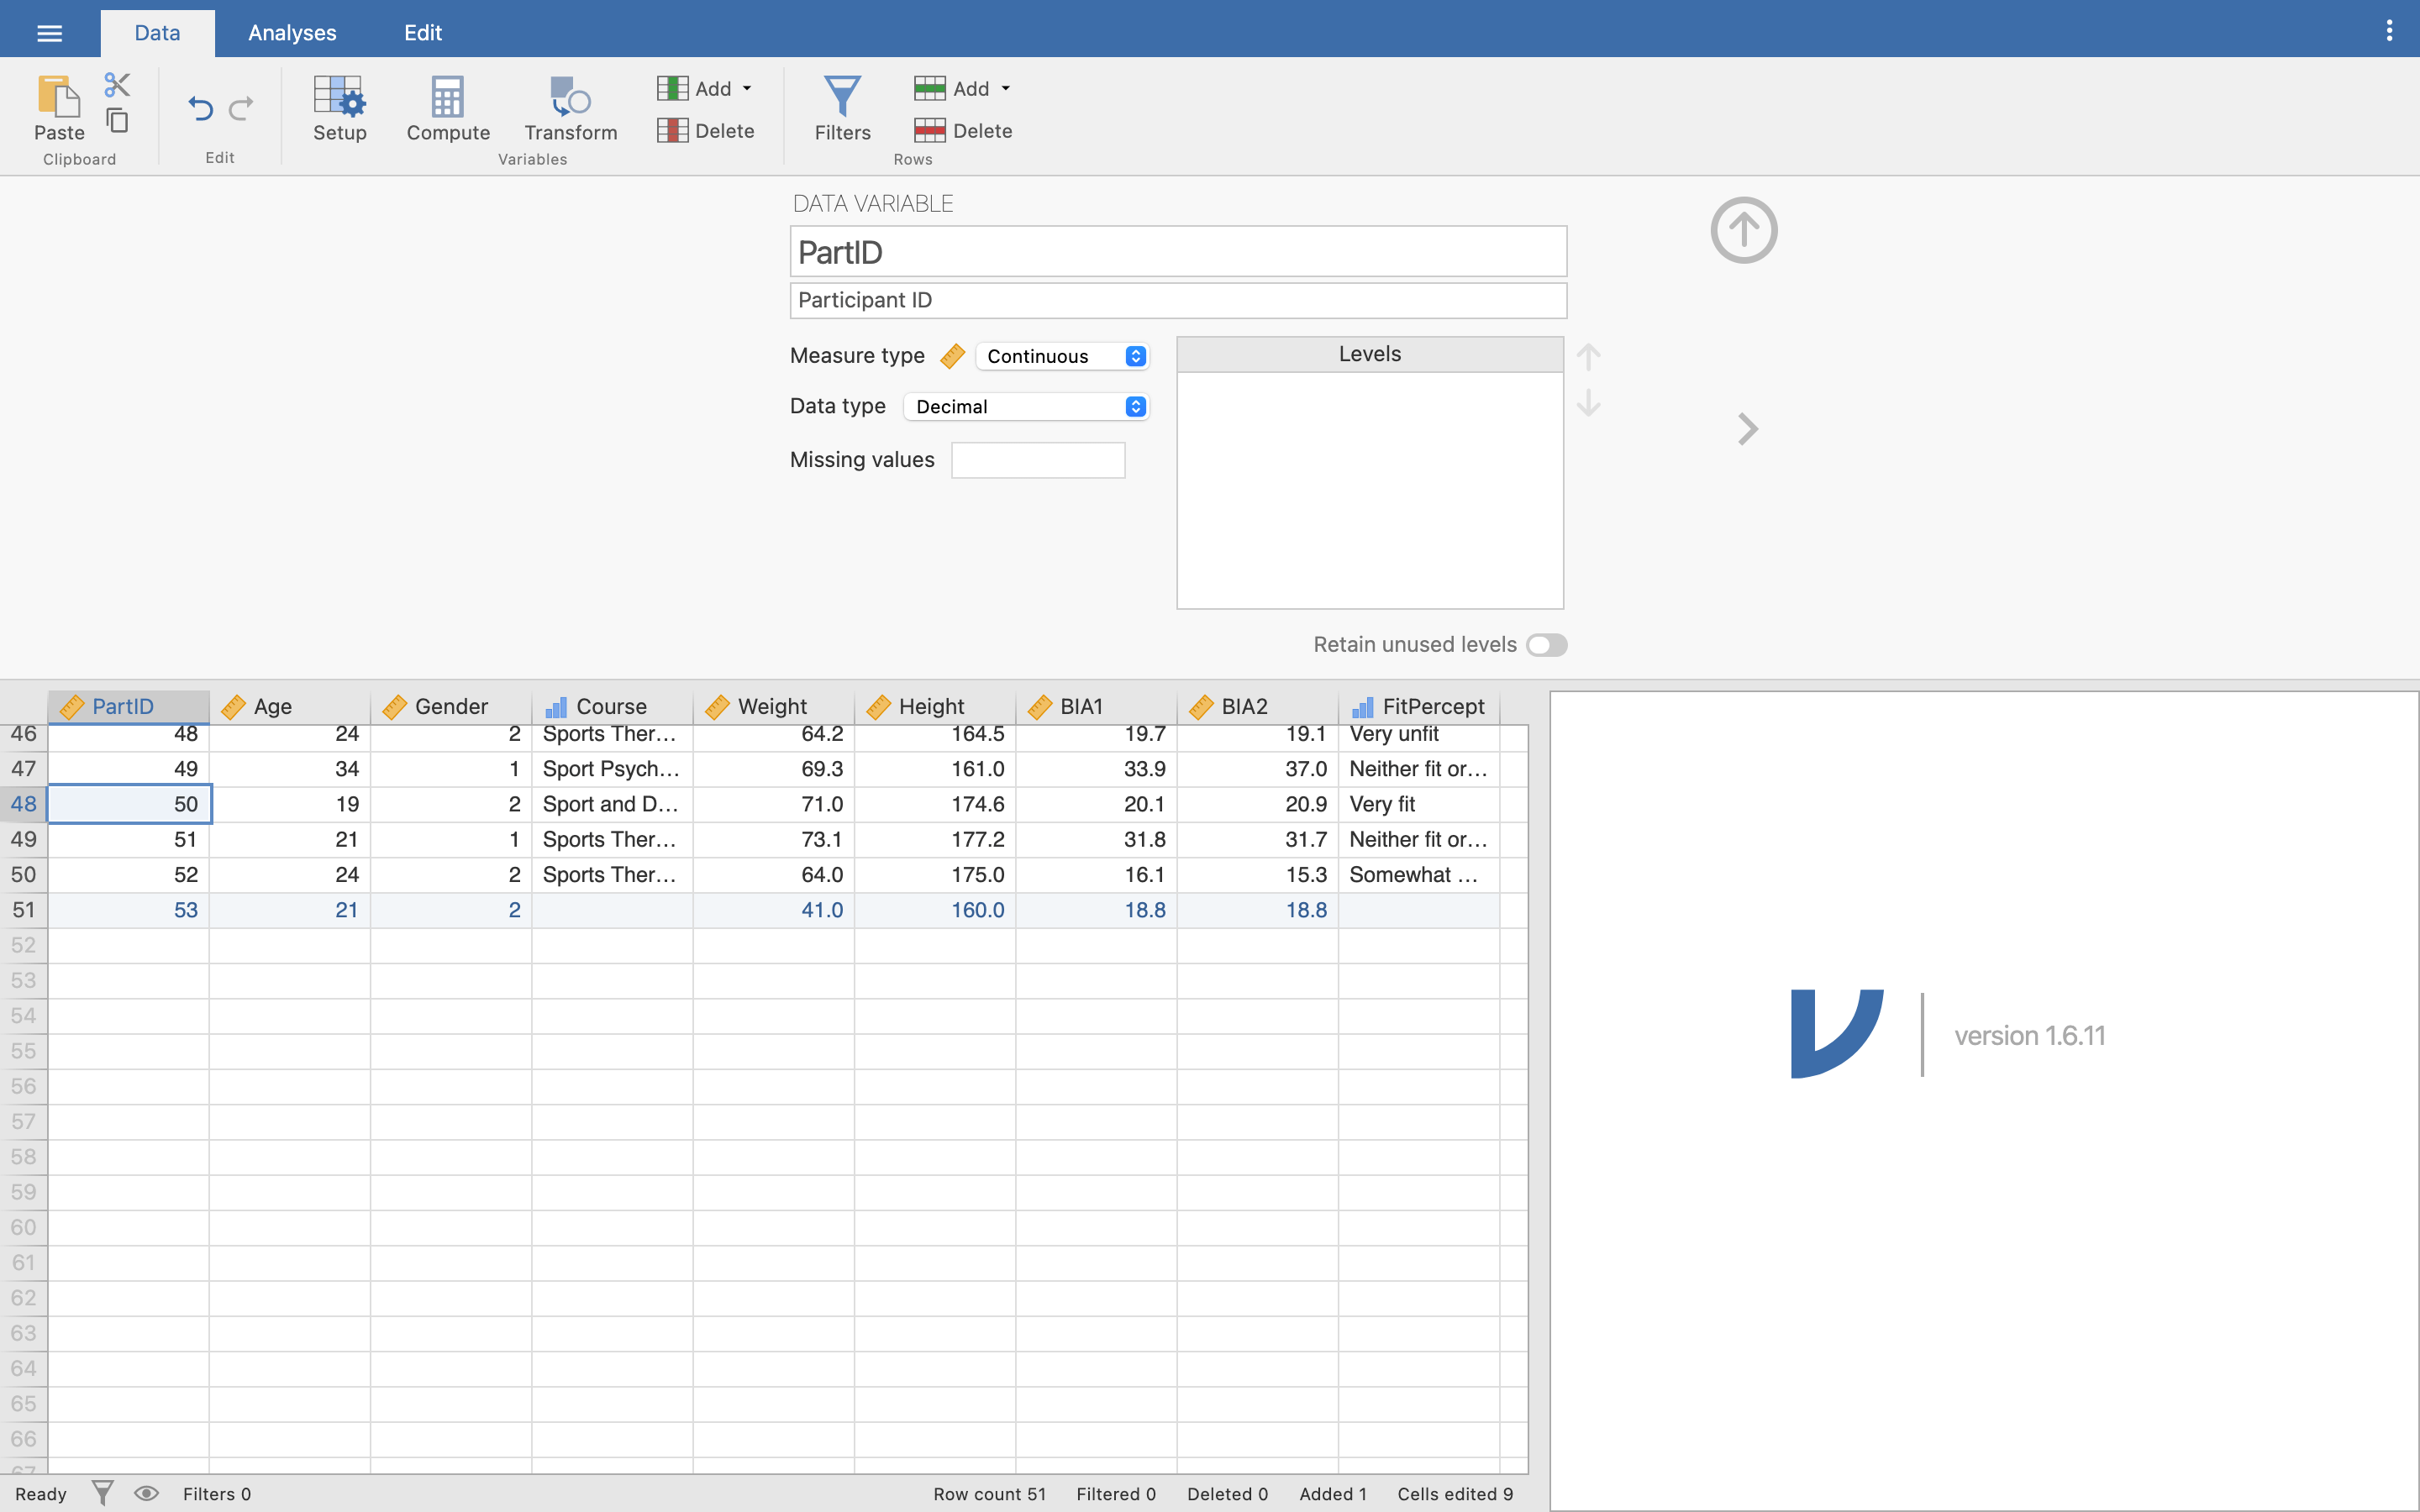
\includegraphics{_imgs/01-04.png}

Bovenaan zie je in grote tekst de naam van de variabele die we aan het
bewerken zijn. Dit is de variabele \textbf{Label}. Klik op een cel in
een andere kolom om naar die variabele te gaan - zie hoe de tekst
bovenaan het menu voor het instellen van variabelen verandert.

Direct onder het grote Label-gebied staat nog een tekstvak - dit is het
\textbf{Beschrijving}-gebied, waar je wat extra tekst kunt toevoegen om
duidelijker te maken wat er in onze variabele staat. Klik op de kolom
PartID en zie hoe er nu `Participant ID' staat - dit is de volledige
naam van de variabele, in plaats van het kortere label `PartID'.

\begin{tcolorbox}[beforeafter skip=1cm, ignore nobreak=true, breakable, colframe=Aside-frame, colback=Aside-bg, coltext=Aside-text, boxsep=2mm, arc=0mm, boxrule=0.5mm]

Waarom gebruiken we aparte labels en beschrijvingen? Wanneer je met een
variabele werkt, kan het soms vervelend zijn om de volledige naam steeds
opnieuw in te typen - `PartID' is veel sneller in te typen dan
`Deelnemer-ID'. Maar als we onze resultaten willen zien, willen we de
volledige beschrijving van de variabele, zodat het makkelijker en
duidelijker is om te zien waar onze resultaten naar verwijzen.

\end{tcolorbox}

Wijzig nu een paar variabele eigenschappen:

\begin{itemize}
\tightlist
\item
  Je ziet dat de meeste van onze variabelen een Naam en Beschrijving
  hebben, maar er ontbreken er twee. Voer voor de kolom \textbf{Age} de
  beschrijving `Age (years)' in en voer voor de kolom \textbf{Gender} de
  beschrijving `Gender' in.
\end{itemize}

\hypertarget{variabele-gegevenstypen}{%
\subsubsection{Variabele gegevenstypen}\label{variabele-gegevenstypen}}

Onder de beschrijving staan nog enkele opties. Klik op het dropdownmenu
naast \textbf{Measure type}:

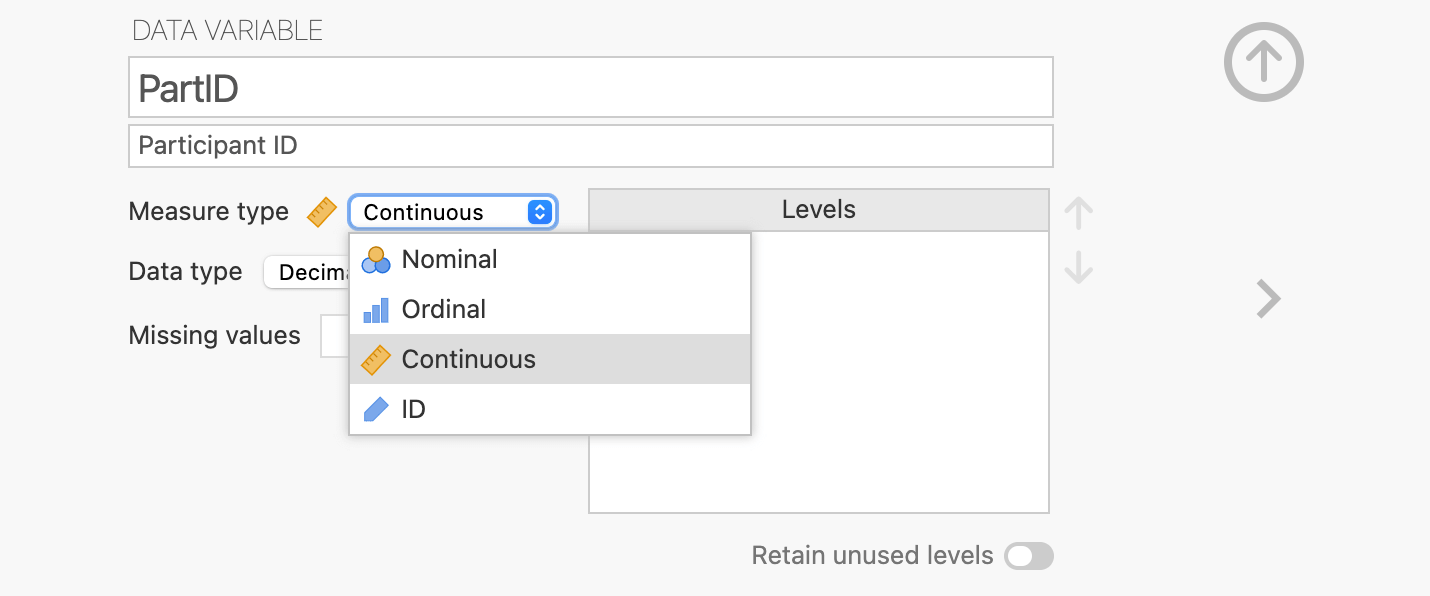
\includegraphics{_imgs/01-05.png}

\begin{tcolorbox}[beforeafter skip=1cm, ignore nobreak=true, breakable, colframe=Questions-frame, colback=Questions-bg, coltext=Questions-text, boxsep=2mm, arc=0mm, boxrule=0.5mm]

\protect\hypertarget{Q5}{\protect\hyperlink{A5}{Q5}}. Hoeveel datatypes
zijn er beschikbaar in Jamovi?

\end{tcolorbox}

Jamovi heeft drie hoofdtypen gegevens:

\begin{itemize}
\tightlist
\item
  Nominaal
\item
  Ordinaal
\item
  Continu
\end{itemize}

Nominaal en Ordinaal zijn precies hetzelfde als de meetniveaus die je
elders vindt. Continu' is gewoon de combinatie van Interval en Ratio -
Jamovi rekent achter de schermen uit of de gegevens die je invoert
Interval of Ratio zijn, op basis van de getallen in de gegevens.

Jamovi heeft ook een extra gegevenstype, genaamd `ID'. Dit wordt gewoon
gebruikt door Jamovi om een Deelnemer ID kolom te identificeren - het is
precies hetzelfde als een Nominale kolom, maar laat Jamovi weten dat het
zich geen zorgen hoeft te maken over het labelen van niveaus en dat het
gewoon moet gebruiken wat er in de cellen wordt getypt. Maak je niet te
veel zorgen over het verschil - weet alleen dat je je PartID kolom
alleen op `ID' hoeft in te stellen.

\begin{tcolorbox}[beforeafter skip=1cm, ignore nobreak=true, breakable, colframe=Questions-frame, colback=Questions-bg, coltext=Questions-text, boxsep=2mm, arc=0mm, boxrule=0.5mm]

\protect\hypertarget{Q6}{\protect\hyperlink{A6}{Q6}}. Waarom zou PartID
van het type ID of Nominal zijn, ook al lijkt het een geordende lijst
van getallen te zijn?

\end{tcolorbox}

Klik onder de opties voor het meetniveau op het vervolgkeuzemenu voor
\textbf{Data type}:

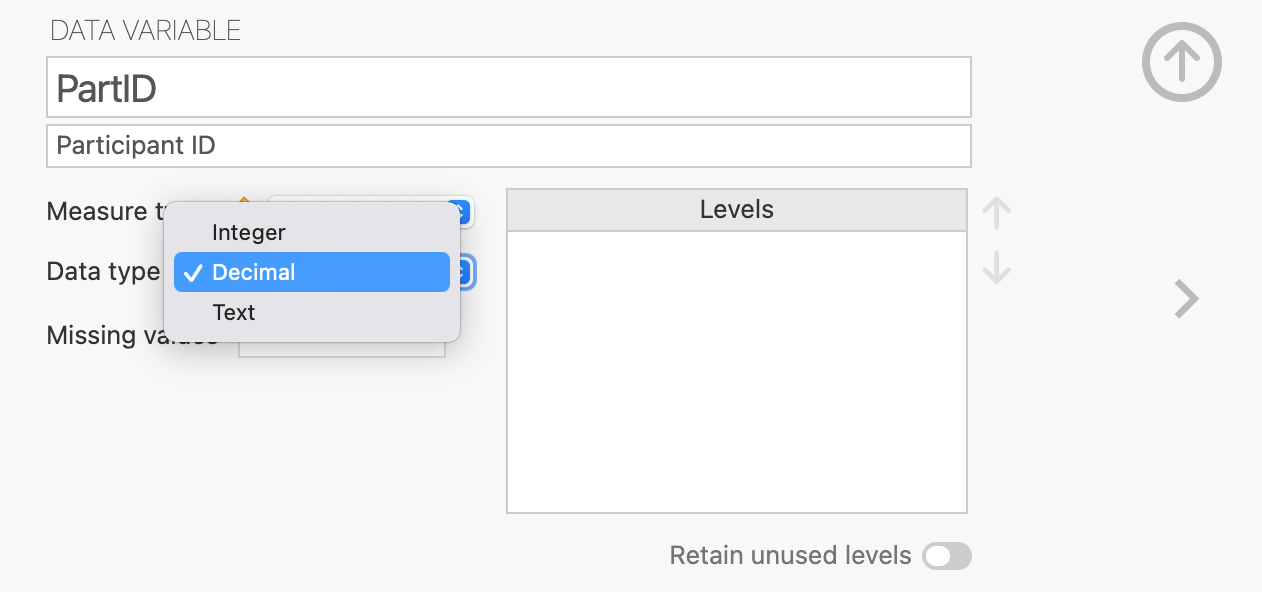
\includegraphics{_imgs/01-06.png}

Gegevenstypen vertellen Jamovi wat voor soort gegevens we gaan invoeren
in de cellen van het gegevensblad. Deze zouden vrij duidelijk moeten
zijn:

\begin{itemize}
\tightlist
\item
  Integer: gehele getallen zonder decimaalteken (1, 2, 3, \ldots)
\item
  Decimal: getallen met een decimaalteken (1.5, 2.3, 3.0, 4.6, \ldots)
\item
  Text: woorden (Ja, Nee, John Smith, voetbal, \ldots)
\end{itemize}

We zullen het gedeelte `Missing values' voorlopig negeren.

\hypertarget{codering-value-labels}{%
\subsubsection{Codering value labels}\label{codering-value-labels}}

Tot slot staat rechtsonder in de variabelenviewer de instelling
\textbf{Levels}. Hier kunnen we, als we categorische gegevens gebruiken
(d.w.z. nominale of ordinale gegevenstypen), de labels instellen die
moeten verschijnen voor elk niveau van die categorie.

Klik bijvoorbeeld op de kolom \textbf{Gender} terwijl het venster
Variable setup geopend staat. Merk op hoe de gegevens worden ingevoerd
als de getallen 1 en 2, in plaats van als tekst. Verander het
\textbf{Measure type} in `Nominal' en je zou de getallen 1 en 2 moeten
zien verschijnen in het vak Levels.

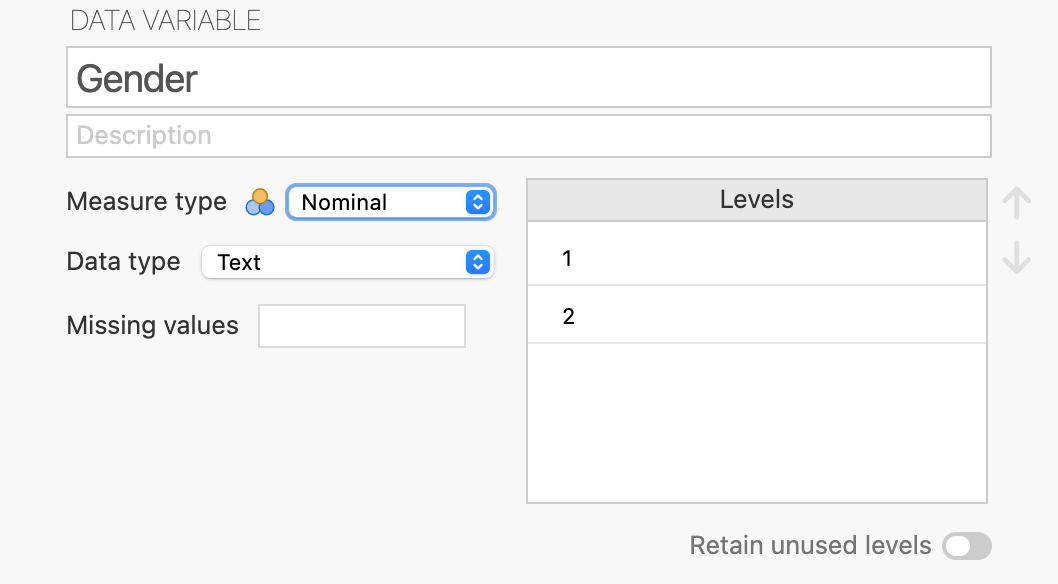
\includegraphics{_imgs/01-07.png}

Klik op het getal 1 in het vak Levels om het label voor deze waarde in
te voeren. Verander dit van een `1' in het woord `Male'. Klik op het
nummer 2 en verander het in `Female'.

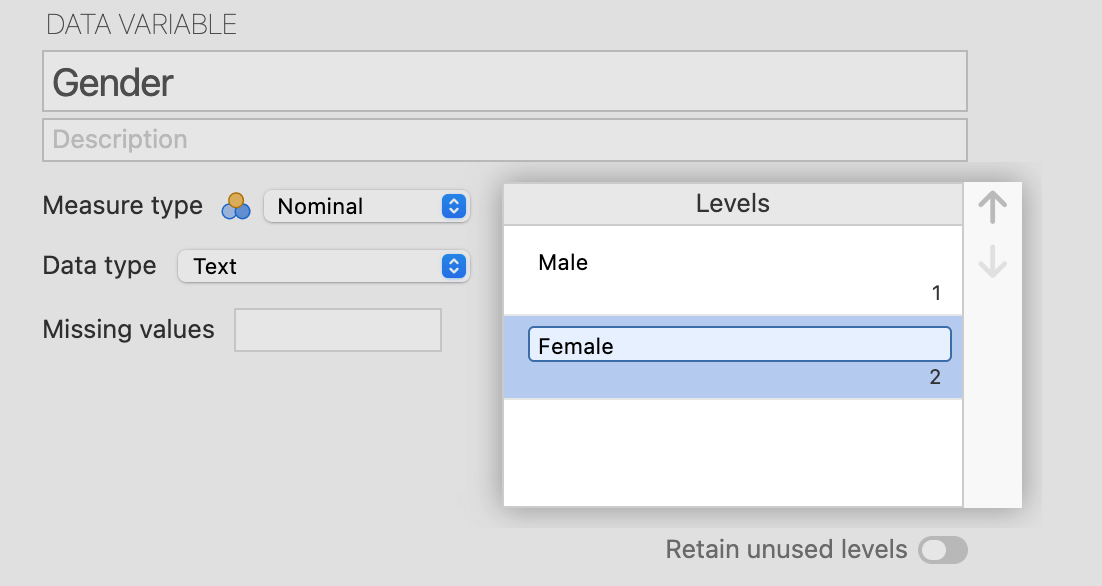
\includegraphics{_imgs/01-08.png}

Merk op hoe de nummers 1 en 2 naar rechtsonder de tekst die je typt
verschuiven, zodat je nog steeds kunt zien welk label naar welk nummer
verwijst. Klik ergens buiten het labelsvak om deze labels op te slaan.

Merk nu op dat de cellen in de kolom Gender in het gegevensblad
veranderen van `1' en `2' in `Male' en `Female'. De onderliggende
gegevens zijn nog steeds hetzelfde - we hebben ze alleen gelabeld.

\begin{tcolorbox}[beforeafter skip=1cm, ignore nobreak=true, breakable, colframe=Aside-frame, colback=Aside-bg, coltext=Aside-text, boxsep=2mm, arc=0mm, boxrule=0.5mm]

Waarom getallen en labels gebruiken voor nominale gegevens? Net als bij
de namen en labels van onze variabelen, maakt het het makkelijker om met
de gegevens te werken en toch onze resultaten duidelijk af te lezen. Als
we bijvoorbeeld alleen de mannelijke deelnemers aan dit onderzoek willen
selecteren, kunnen we filteren op `Gender = 1', maar onze resultaten
zouden nog steeds het volledige label `Male' bevatten.

\end{tcolorbox}

Ga nu door en controleer of alle variabelen in ons gegevensblad correct
zijn ingesteld. Zorg ervoor dat de variabelen overeenkomen met de
volgende:

\begin{itemize}
\tightlist
\item
  Age: Age (years), Continuous, Integer
\item
  Gender: Gender, Nominal, Integer, with 2 levels
\item
  Course: Course Name, Nominal, Integer, with 4 levels
\item
  Weight: Weight (kg), Continuous, Decimal
\item
  Height: Height (cm), Continuous, Decimal
\item
  BIA1: BIA Machine 1 Body Fat (\%), Continuous, Decimal
\item
  BIA2: BIA Machine 2 Body Fat (\%), Continuous, Decimal
\item
  FitPercept: Fitness Perception, Nominal, Integer, with 5 levels
\end{itemize}

Als je al deze variabelen hebt ingesteld, klik je op het cirkelpictogram
met een pijl omhoog rechtsboven in het menu voor het instellen van
variabelen om het menu te verbergen en terug te keren naar de
hoofdweergave.

Zorg ervoor dat je je gegevens regelmatig opslaat - klik op de drie
witte lijnen linksboven om het menu File weer te openen en klik
vervolgens op \textbf{Save}.

\begin{tcolorbox}[beforeafter skip=1cm, ignore nobreak=true, breakable, colframe=Tip-frame, colback=Tip-bg, coltext=Tip-text, boxsep=2mm, arc=0mm, boxrule=0.5mm]

Gebruik Ctrl + S in Windows of Cmd + S op Mac als sneltoets om je werk
op te slaan. Zorg ervoor dat je regelmatig opslaat om te voorkomen dat
je iets kwijtraakt! Al je gegevens, tests en resultaten worden
opgeslagen in hetzelfde .omv-bestand, zodat je het later weer kunt
openen en verder kunt gaan waar je gebleven was.

\end{tcolorbox}

\hypertarget{een-nieuwe-variabele-berekenen}{%
\subsubsection{Een nieuwe variabele
berekenen}\label{een-nieuwe-variabele-berekenen}}

We ontbreken nog een BMI-variabele, dus gaan we er een maken. Je zou
alle gegevens in Excel kunnen maken en ze dan kopiëren en plakken in
Jamovi, maar Jamovi heeft een functie \textbf{Compute variable} die de
berekening voor ons kan uitvoeren.

Klik op de kolom \textbf{FitPercept}, klik vervolgens op \textbf{Data}
en vervolgens op \textbf{Compute} (het pictogram dat eruitziet als een
rekenmachine). Dit voegt een nieuwe kolom toe na de kolom waar onze
cursor staat (daarom hebben we eerst op FitPercept geklikt) en opent het
menu \textbf{Computed variabele} bovenaan, vergelijkbaar met het menu
voor het instellen van variabelen:

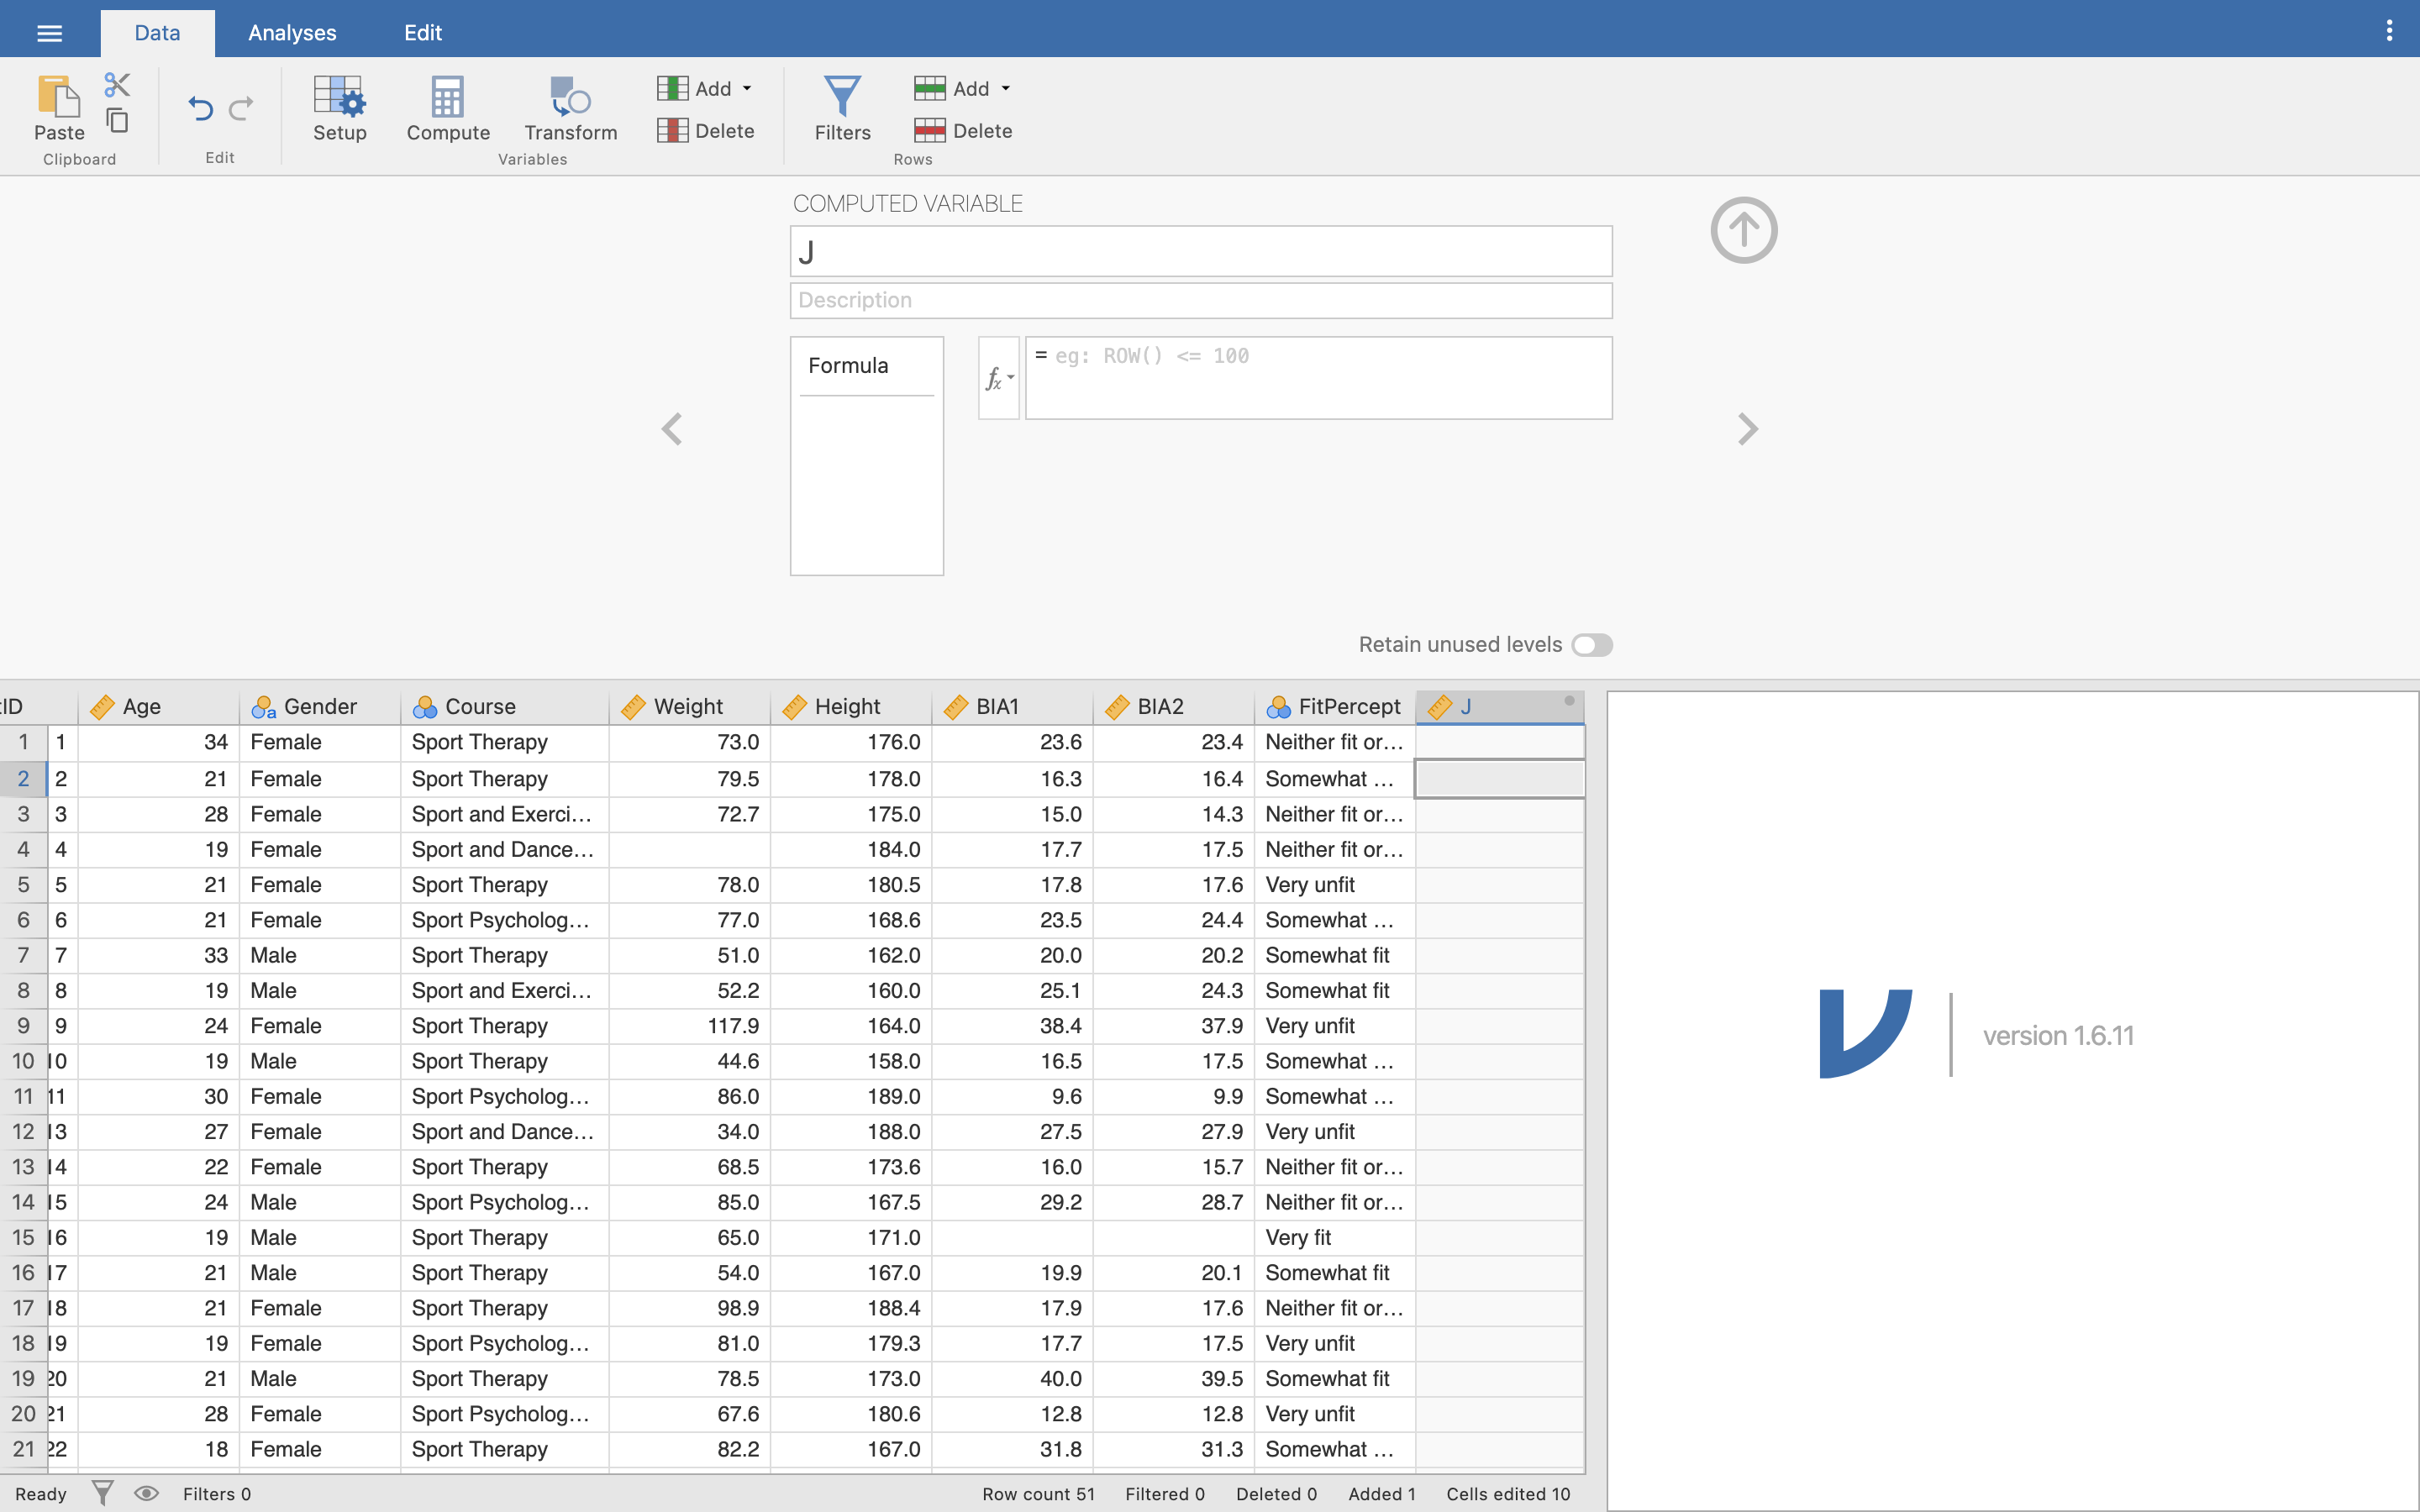
\includegraphics{_imgs/01-09.png}

Jamovi geeft onze variabele automatisch een letter van het alfabet als
naam - `J' in dit geval. Verander de nieuwe variabelenaam in
\textbf{BMI} en voer vervolgens \textbf{Body Mass Index} in als
beschrijving.

Onder de naam en beschrijving staat het vak \textbf{formule box}. Hier
voeren we een formule in om Jamovi te vertellen wat hij voor ons moet
berekenen - heel vergelijkbaar met wanneer we functies in Excel typen,
maar in plaats van ze in één cel te typen en de formule in alle andere
cellen te kopiëren en plakken, voeren we in Jamovi gewoon de functie
bovenaan in en wordt deze automatisch voor de hele kolom voor ons
ingevuld.

We kunnen direct in het formulevak typen of Jamovi sommige delen voor
ons laten invullen. Klik op de \textbf{fx} knop om alle opties te zien
die we in het formulevak kunnen invoeren:

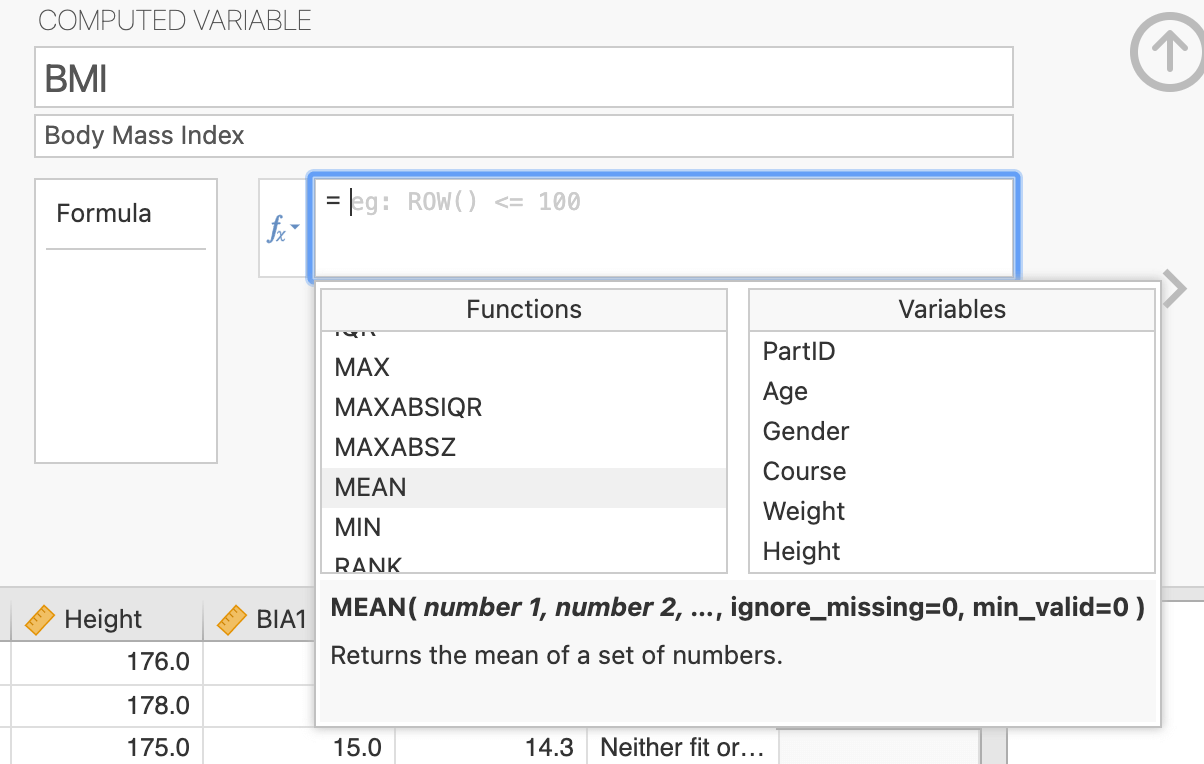
\includegraphics{_imgs/01-10.png}

Jamovi vertelt ons wat elke functie doet als we er één keer op klikken -
zie hier dat ik op de MEAN-functie heb geklikt, en Jamovi geeft er een
korte beschrijving onder. Naast de functies staan onze variabelen.
Dubbelklik op deze variabelen om ze in te voegen in het functievak.

Typ of kopieer en plak nu het volgende in het functievak:

\begin{verbatim}
Weight / ((Height/100) * (Height / 100))
\end{verbatim}

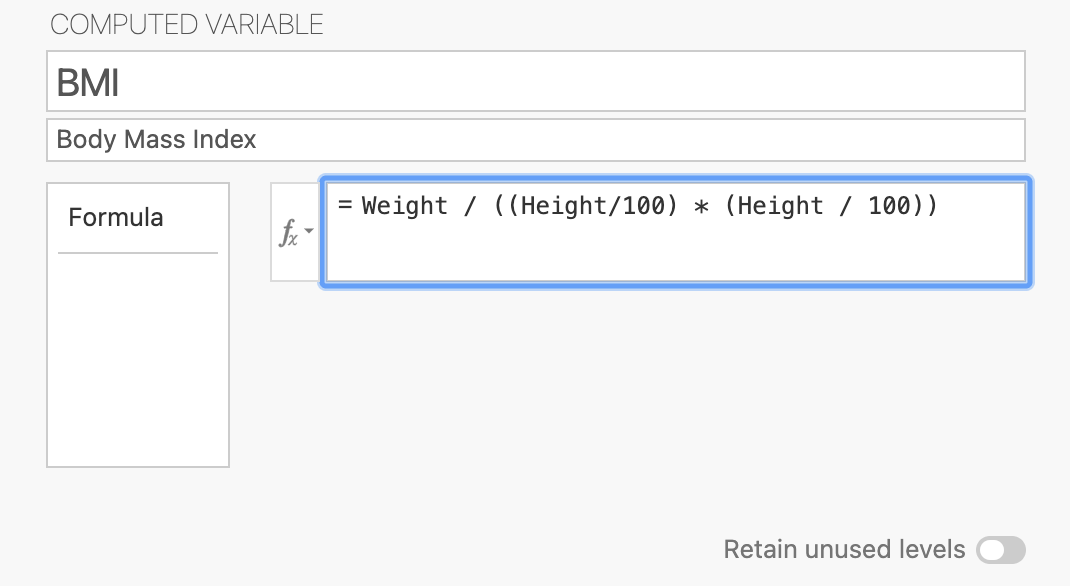
\includegraphics{_imgs/01-11.png}

Druk op enter en je zou moeten zien dat de BMI kolom automatisch wordt
ingevuld met onze BMI waarden. Merk op dat alle cases (rijen) die geen
gewichts- of lengtegegevens hebben, ook leeg blijven in de nieuwe
BMI-kolom.

\textbf{Even samenvatten:} we hebben gekeken naar het gegevensblad dat
onze gegevens (cellen) bevat gerangschikt als Variabelen (kolommen) en
Cases (rijen). We hebben in het menu Variable Setup gekeken naar de
metadata-informatie over onze variabelen en de waarden die ze bevatten.
Dit zijn de twee hoofdcomponenten van wat we gegevens zouden noemen.

De variabelen en de gegevens worden allemaal opgeslagen in één
Jamovi-gegevensbestand (.omv). Zorg ervoor dat je je gegevensbestand
opslaat wanneer je wijzigingen hebt aangebracht in zowel de variabelen
als de cases. We gaan nu verder met het onderzoeken van enkele van onze
gegevens.

\begin{tcolorbox}[beforeafter skip=1cm, ignore nobreak=true, breakable, colframe=Aside-frame, colback=Aside-bg, coltext=Aside-text, boxsep=2mm, arc=0mm, boxrule=0.5mm]

Gebruik het \textbf{File} menu van eerder om je werk op te slaan - klik
op de drie gestapelde witte lijnen in de hoek en kies \textbf{Save} of
\textbf{Save as}. U kunt ook de sneltoetsen \textbf{Ctrl + S} (Windows)
of \textbf{Cmd + S} (Mac) gebruiken om op te slaan.

\end{tcolorbox}

\newpage{}

\hypertarget{descriptives-plots-and-parametric-testing}{%
\section{Descriptives, plots, and parametric
testing}\label{descriptives-plots-and-parametric-testing}}

Now that we have our data setup in Jamovi, we can start investigating it
with some descriptives, some basic plots, and some parametric testing.

\hypertarget{descriptive-data}{%
\subsection{Descriptive data}\label{descriptive-data}}

In the Excel class we took a lot of time looking at descriptive data.
This is information about your data, for instance, the total number of
records, the minimum, maximum, range, standard deviation, etc. Jamovi
can provide this information a lot quicker than us calculating it
ourselves each time. Here we are going to use some the Exploration
analyses to help describe our data.

In the \textbf{Analyses} menu, click on the \textbf{Explore} icon (that
looks like a bar graph), then click \textbf{Descriptives} in the
dropdown menu that appears. A new middle area should open up between our
Spreadsheet and Results Viewer:

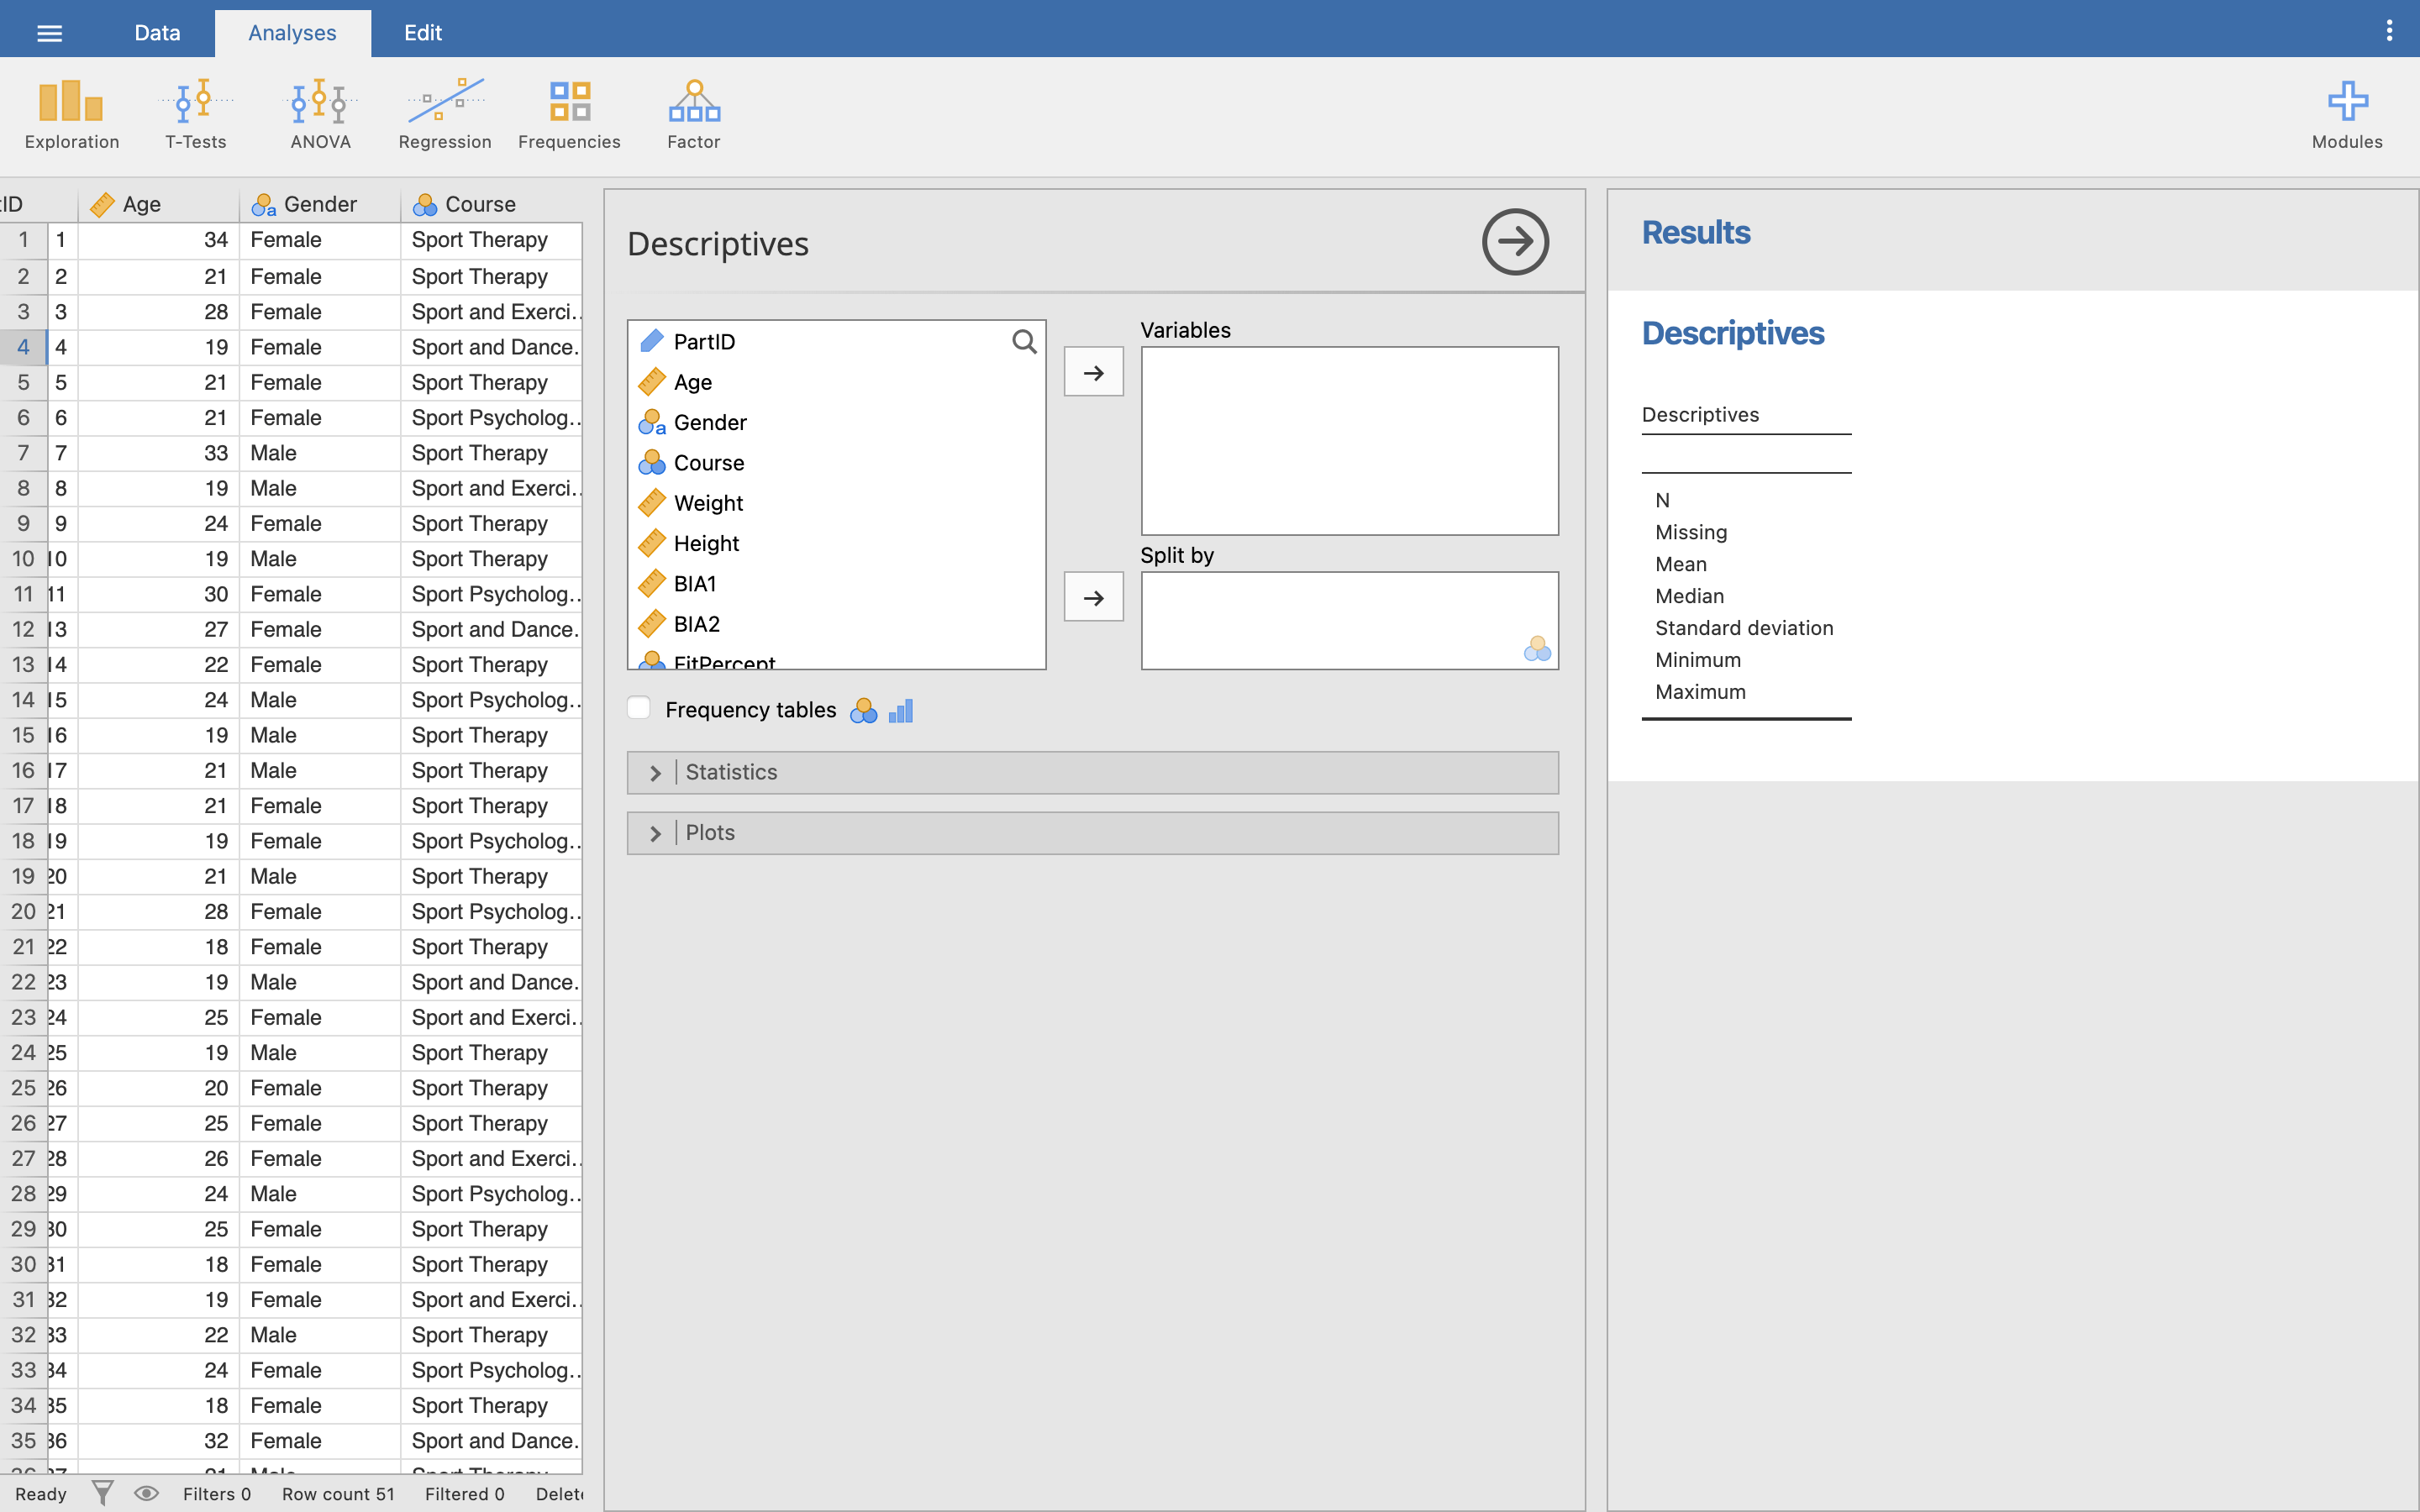
\includegraphics{_imgs/01-12.png}

Notice that something has also showed up on our Results Viewer! This is
how Jamovi works - when you run an Analyses, the results are printed out
onto the viewer on the right. The Descriptives Analyses prints out a
table of information by default, but at the moment, we haven't told
Jamovi exactly what we want Descriptives of yet, so the table is empty.

Click on the \textbf{Weight} variable in the left hand box, and click
the arrow to move it into the \textbf{Variables} box on the right. Then,
click on the \textbf{Gender} variable, and use the arrow to move it
across to the \textbf{Split By} section:

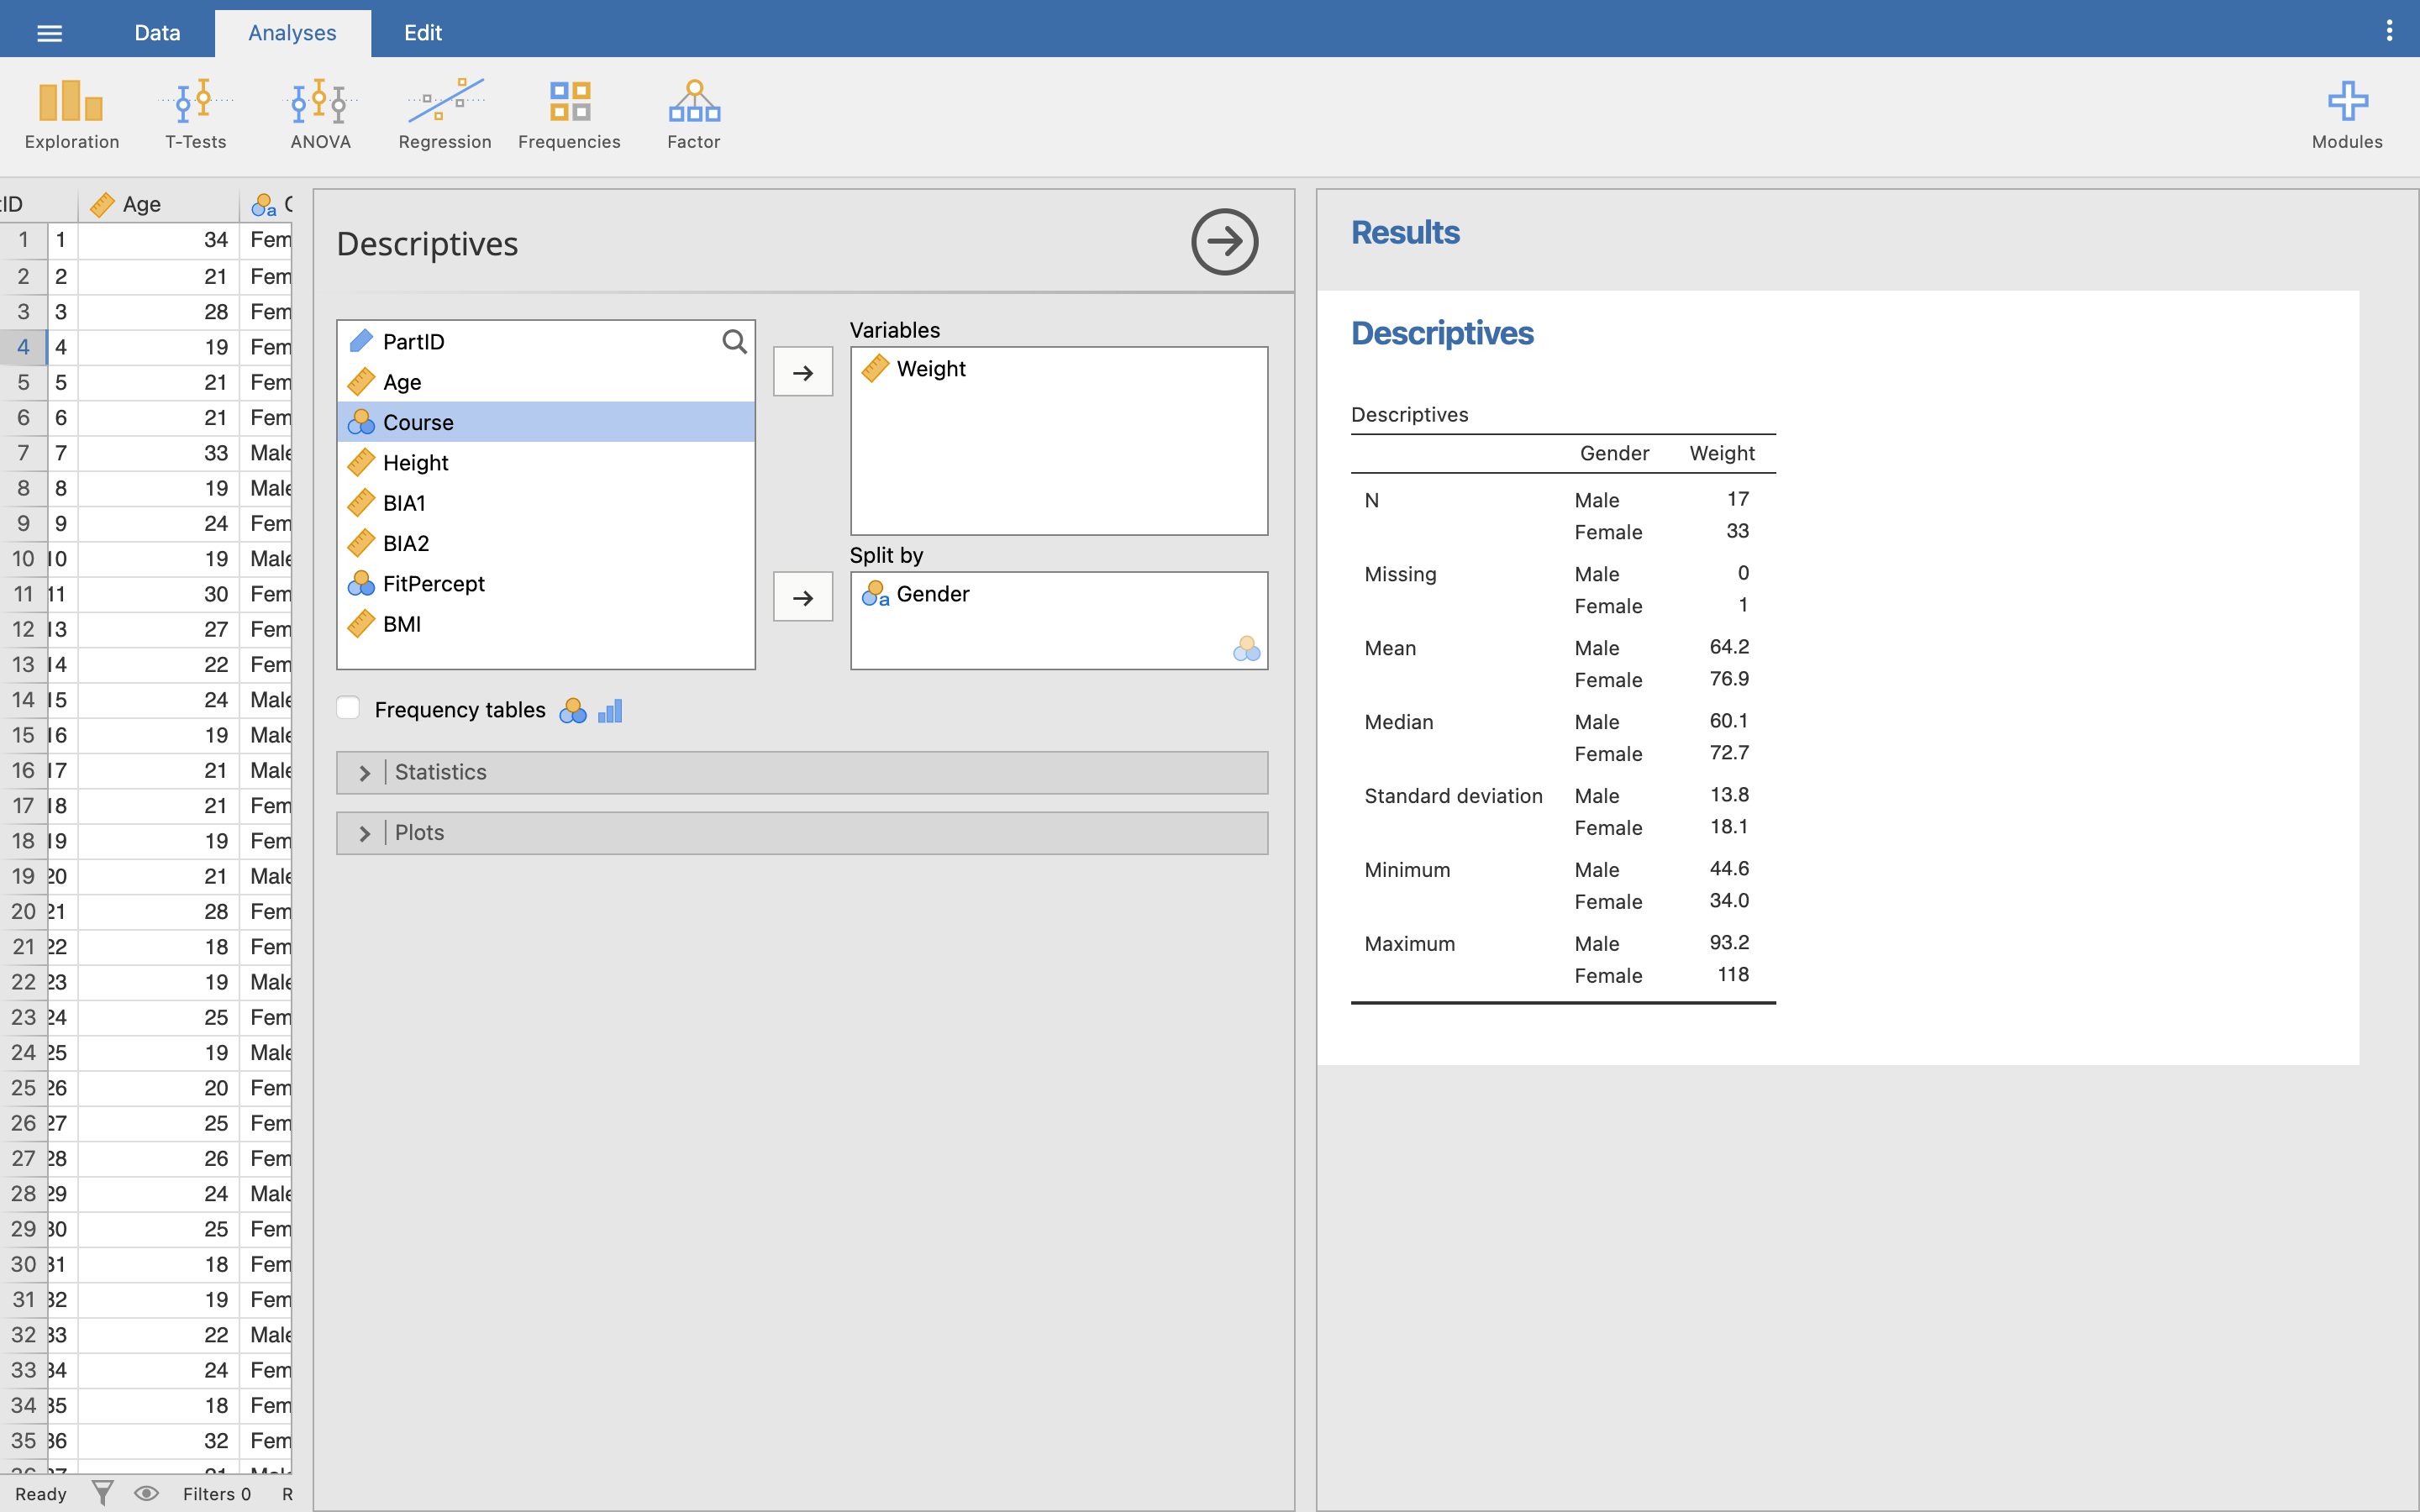
\includegraphics{_imgs/01-13.png}

This is a simple way of looking at all the weights of our participants
(dependent list) broken down by gender (factor list).

Notice our Results table on the right has now automatically updated to
show the Descriptives we have asked for! You should be able to see the
mean, median, standard deviation, minimum, and maximum for both Male and
Female groups. All of these require separate equations in Excel, so you
can see Jamovi is a \emph{lot} quicker to summarise data.

\begin{tcolorbox}[beforeafter skip=1cm, ignore nobreak=true, breakable, colframe=Questions-frame, colback=Questions-bg, coltext=Questions-text, boxsep=2mm, arc=0mm, boxrule=0.5mm]

\protect\hypertarget{Q7}{\protect\hyperlink{A7}{Q7}}. In your
descriptive data who, on average is heavier, male or female?

\protect\hypertarget{Q8}{\protect\hyperlink{A8}{Q8}}. How many males and
females are there? And how big is our total sample size?

\end{tcolorbox}

Let's look at some more of our data. Previously I mentioned we had two
columns, BIA1 and BIA2, where we took the body fat percentage using two
`identical' machines. Here we can briefly examine these two fields to
compare any differences.

Click on \textbf{Weight} in the Variables area and notice the arrow icon
changes to point left - click this to put it back into our variables
list. Do the same for \textbf{Gender}. The table in our Results viewer
should go empty again.

Now select \textbf{BIA1} and \textbf{BIA2} and move them into the
Variables box. This will show the same information as before, but now we
want a little bit extra. Click on the \textbf{Statistics} dropdown menu
below our variables selector to see all the various statistics we can
ask Jamovi to show us. Click on \textbf{Range} to add it to our table in
the Results viewer:

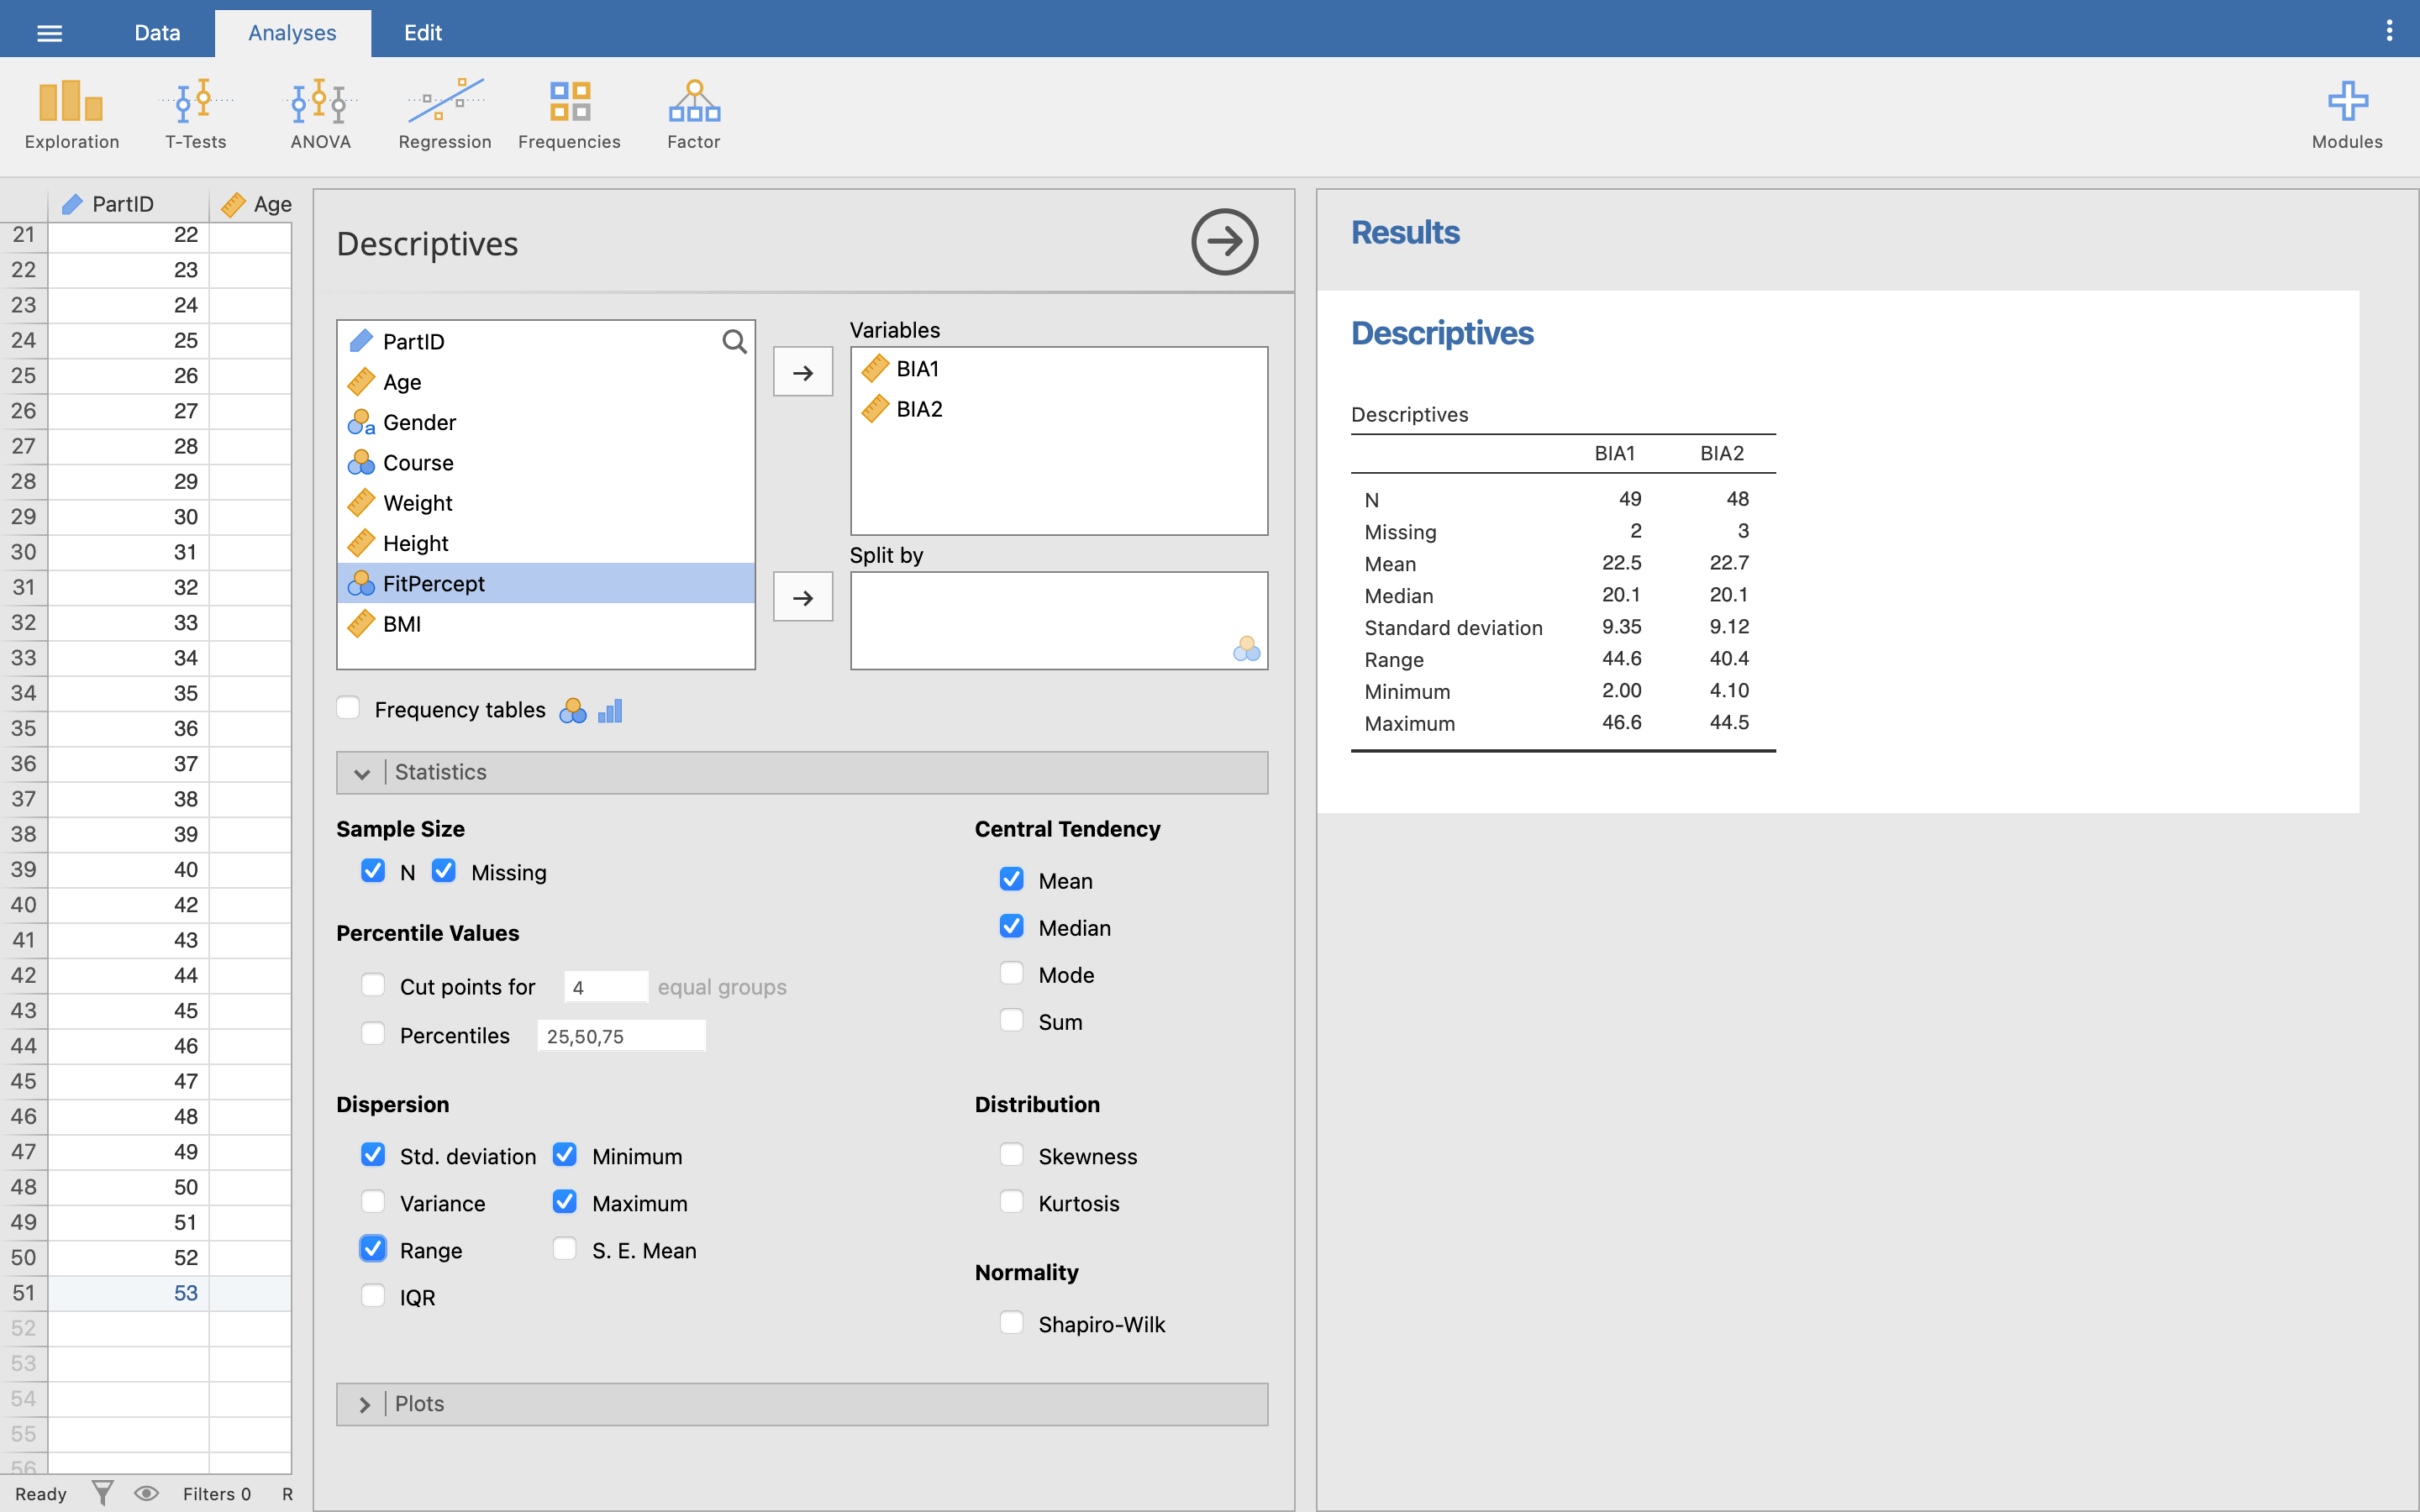
\includegraphics{_imgs/01-14.png}

Feel free to click around any other Statistics options you might be
interested in - you can add and remove as many as you like at any time
in Jamovi, and the Results viewer will auto-update to show what you have
changed.

\begin{tcolorbox}[beforeafter skip=1cm, ignore nobreak=true, breakable, colframe=Questions-frame, colback=Questions-bg, coltext=Questions-text, boxsep=2mm, arc=0mm, boxrule=0.5mm]

\protect\hypertarget{Q9}{\protect\hyperlink{A9}{Q9}}. From the
descriptive data for the two machines, would you say the machines show
the `same' results?

\end{tcolorbox}

\hypertarget{frequency-tables}{%
\subsubsection{Frequency tables}\label{frequency-tables}}

Let's also see how many students are on each of the four courses
offered. Move BIA1 and BIA2 out of the variables selected, then move
\textbf{Course} into the variables selection box.

Click the \textbf{Frequency tables} checkbox underneath our variables
selection to add a frequency table to our Results viewer (this will only
work for Nominal or Ordinal data types). If you want to make the Results
viewer a bit tidier, untick all the other Statistics options, but leave
in the \textbf{N} and \textbf{Missing} options:

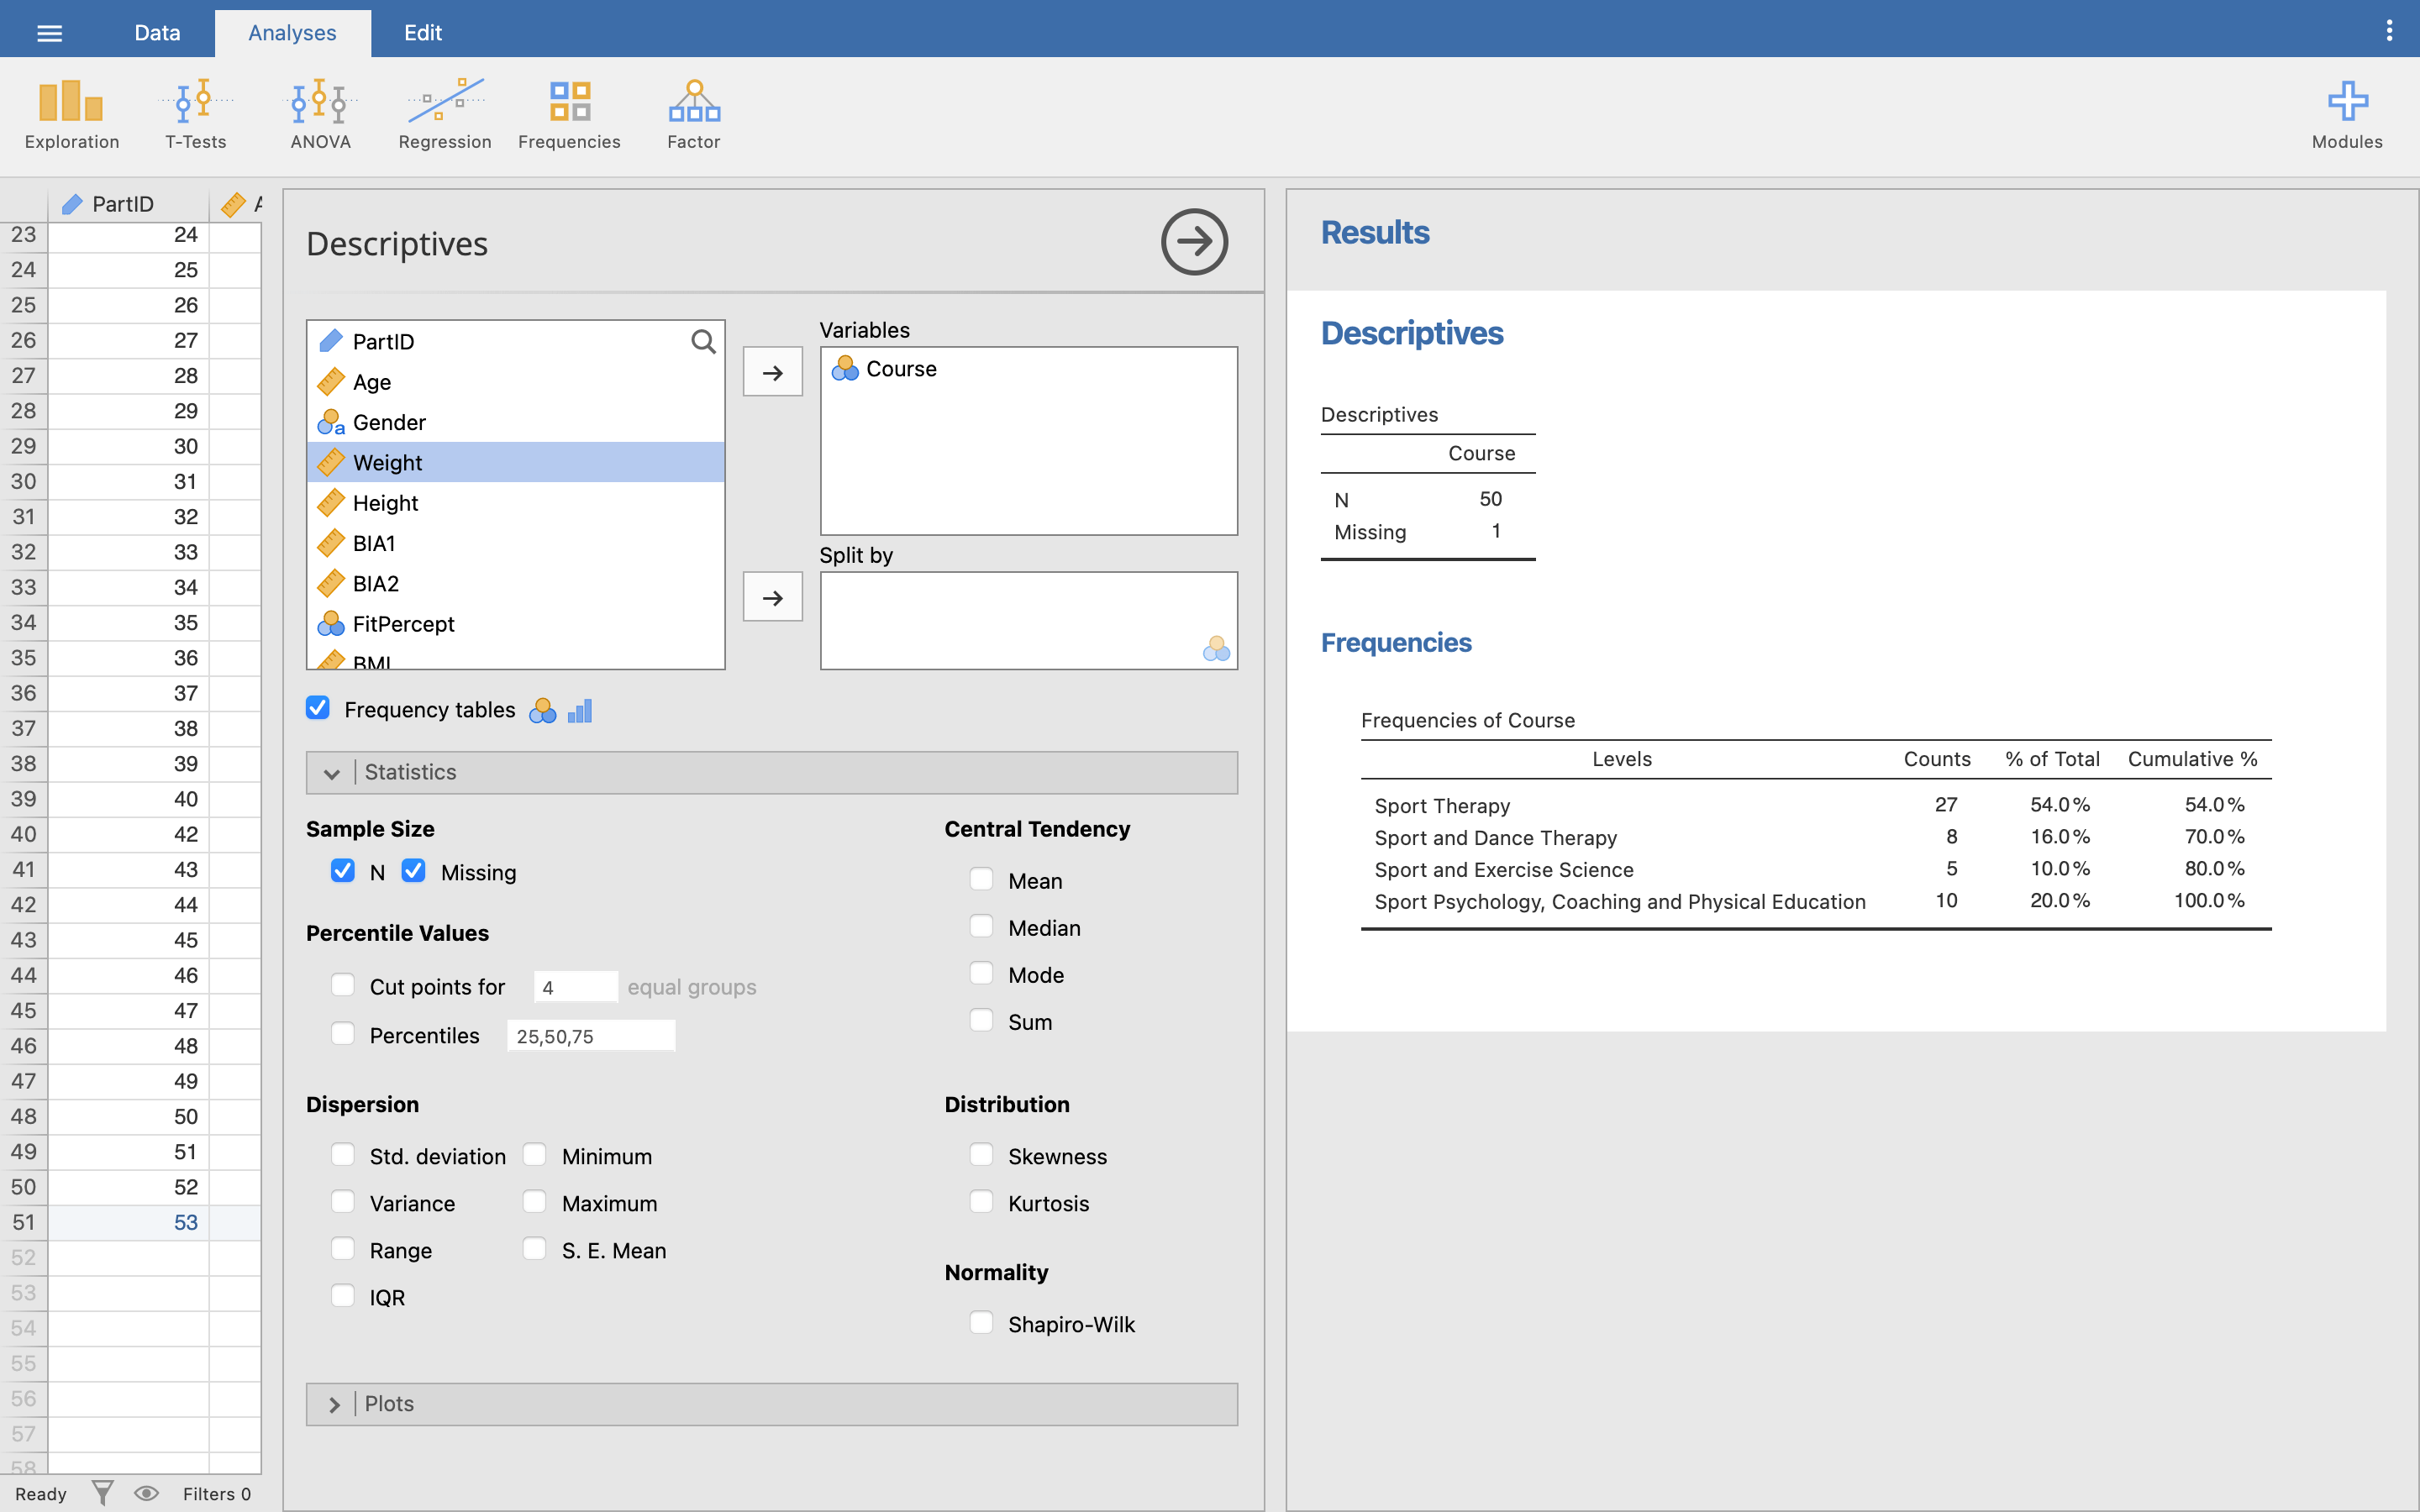
\includegraphics{_imgs/01-15.png}

Here you are presented with frequency as a count, as an overall
percentage, and as a cumulative percentage. Top table also tells us
about the total number of values and how many are missing values - that
is, any cases we have that do not have a valid Course ID.

\begin{tcolorbox}[beforeafter skip=1cm, ignore nobreak=true, breakable, colframe=Questions-frame, colback=Questions-bg, coltext=Questions-text, boxsep=2mm, arc=0mm, boxrule=0.5mm]

\protect\hypertarget{Q10}{\protect\hyperlink{A10}{Q10}}. How many
students actually provided a course id?

\protect\hypertarget{Q11}{\protect\hyperlink{A11}{Q11}}. Which course
has the greatest percentage of students?

\protect\hypertarget{Q12}{\protect\hyperlink{A12}{Q12}}. What percentage
of students takes Sport and Dance Therapy?

\end{tcolorbox}

Notice that our counts in the Frequency table add up to the number of
valid Course IDs we have in our data. You need to make sure you always
check for any missing values in your data - in this case, you might need
to go back and find that missing Course ID, or else exclude the case
from any further analyses if Course ID is required.

\hypertarget{basic-plots}{%
\subsection{Basic plots}\label{basic-plots}}

\hypertarget{histogram}{%
\subsubsection{Histogram}\label{histogram}}

While we expect you to generate graphs in Excel, and produce tables in
MS-Word, you can still generate graphs in Jamovi for a quick view of
data before formatting them in Excel. Remember, for any coursework, it
is generally best to create your final graphs in Excel so you can
completely customise how they look.

We will look at two graphs:

\begin{itemize}
\tightlist
\item
  Histogram
\item
  Box plot
\end{itemize}

We will continue to use our Body Composition.omv data set. Still in the
\textbf{Descriptive} menu, clear all the variables from our variable
selection, and untick the Frequency table option. Move \textbf{Weight}
into the variables selection and turn back on the Default descriptive
statistics - tick the boxes for N, Missing, Mean, Median, Std.
Deviation, Minimum, and Maximum.

Then, you can click the Statistic menu bar again to fold it out of the
way, and click on the \textbf{Plots} menu bar. Click on
\textbf{Histogram} to generate a simple histogram in our Results viewer.

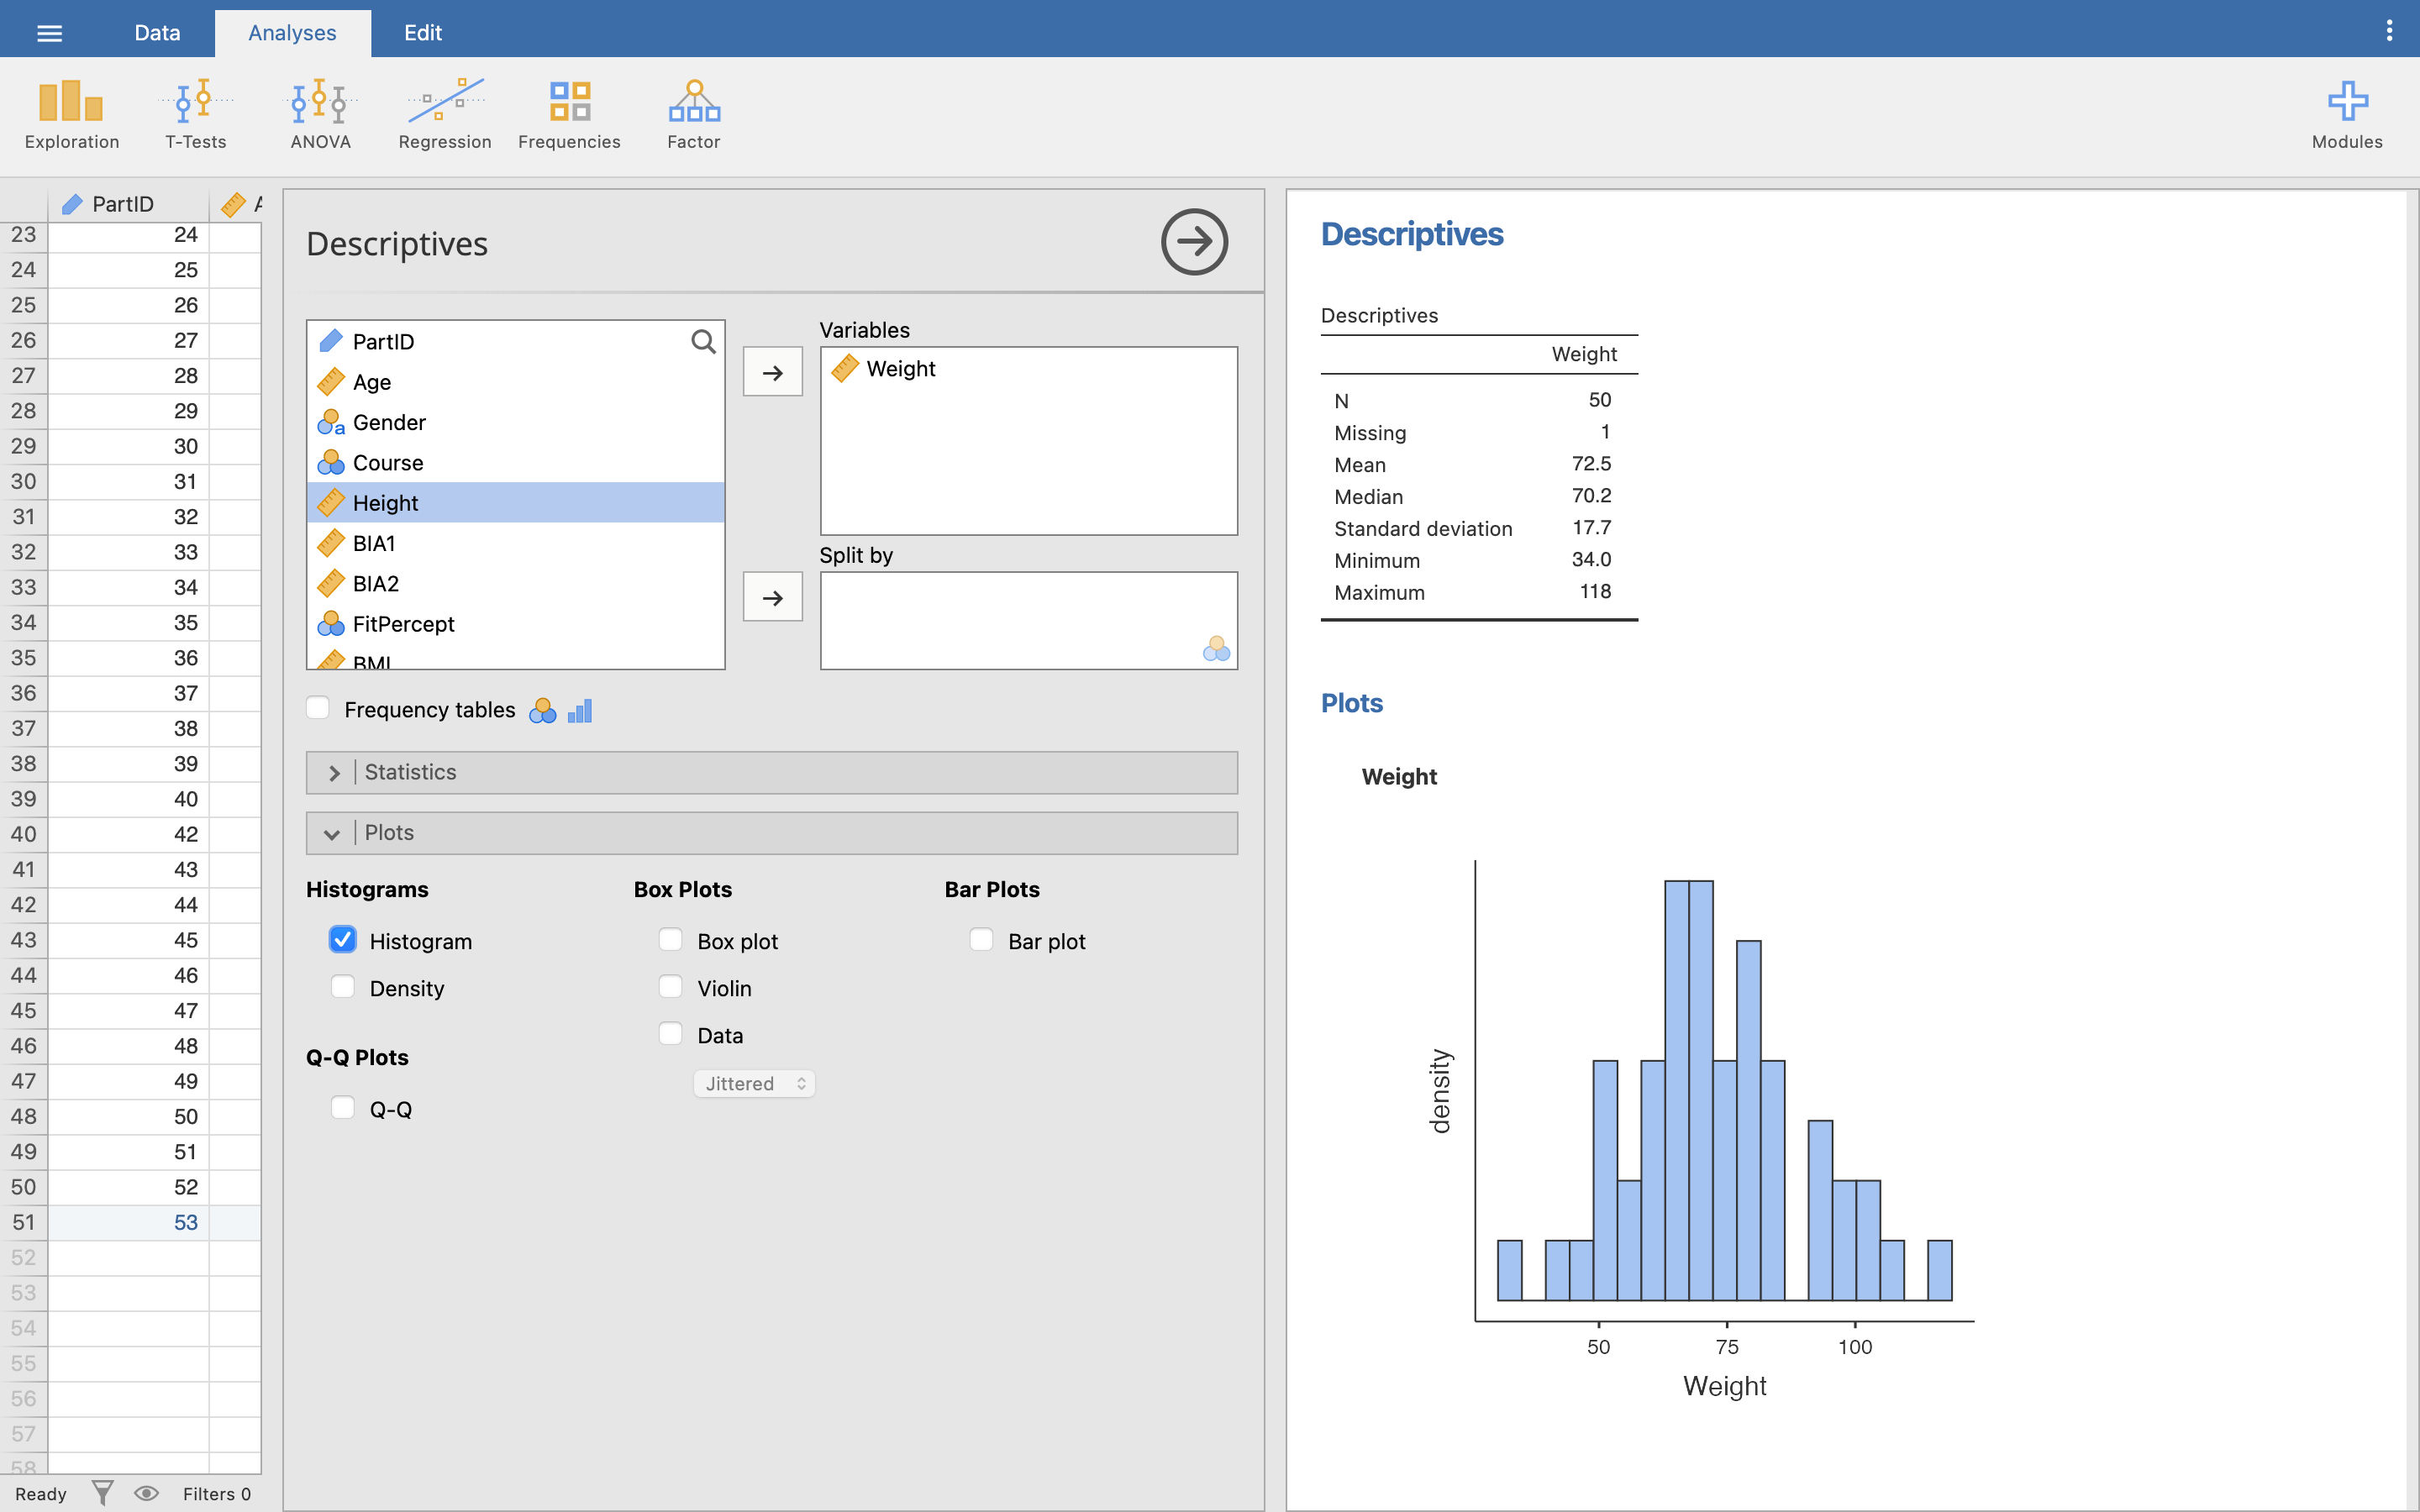
\includegraphics{_imgs/01-16.png}

This is a histogram for our entire data set, but we can split this by
\textbf{Gender} exactly as we did for the Descriptives. Move Gender into
the Split By box and see what happens to our histogram:

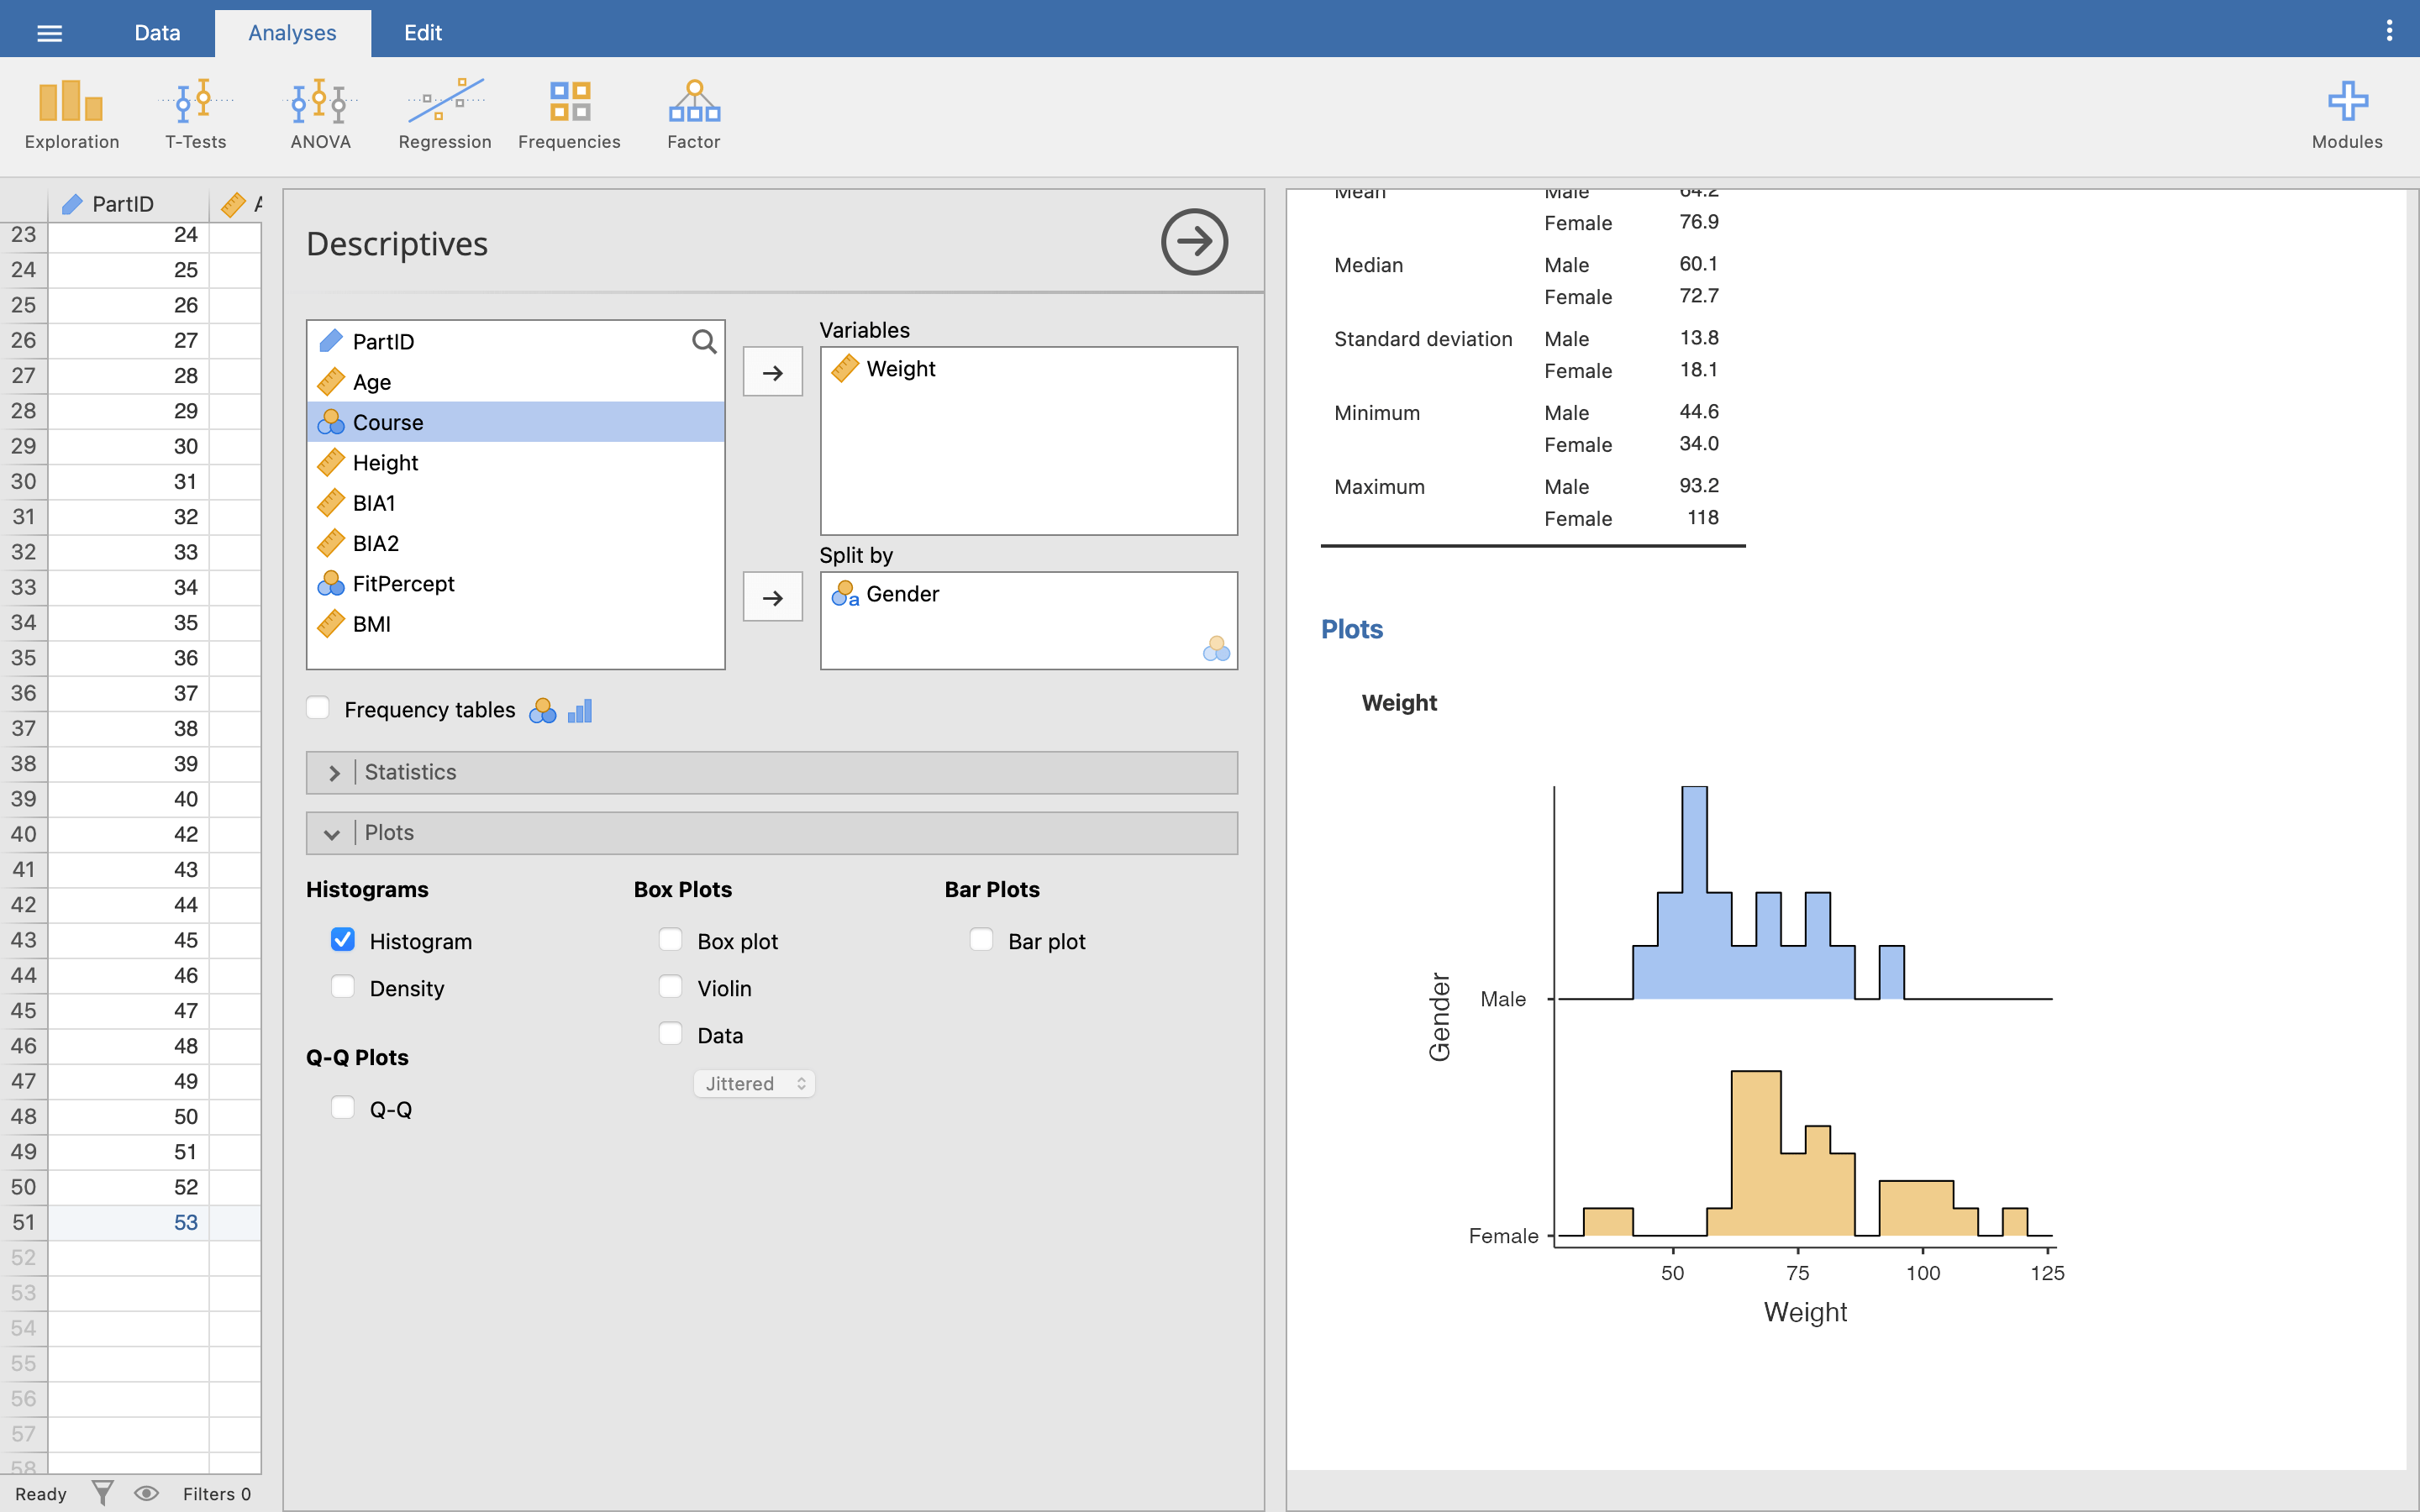
\includegraphics{_imgs/01-17.png}

You can split your data using any Nominal or Ordinal variable - try
moving other variables in and out of the Split By box to see how the
histogram changes.

\begin{tcolorbox}[beforeafter skip=1cm, ignore nobreak=true, breakable, colframe=Questions-frame, colback=Questions-bg, coltext=Questions-text, boxsep=2mm, arc=0mm, boxrule=0.5mm]

\protect\hypertarget{Q13}{\protect\hyperlink{A13}{Q13}}. Based on the
histograms, which Gender has a greater variability of weight? Why?

\end{tcolorbox}

\hypertarget{box-plots}{%
\subsubsection{Box plots}\label{box-plots}}

Boxplots may also be useful to visually inspect your data, especially if
you are looking for outliers. We will use a box plot to check for any
outliers in our height data. Clear the selection boxes, then move
\textbf{Height} into the variables selection, and Split By
\textbf{Gender} again. Then, click the \textbf{Box plot} tick box to
show a box plot in the Results viewer:

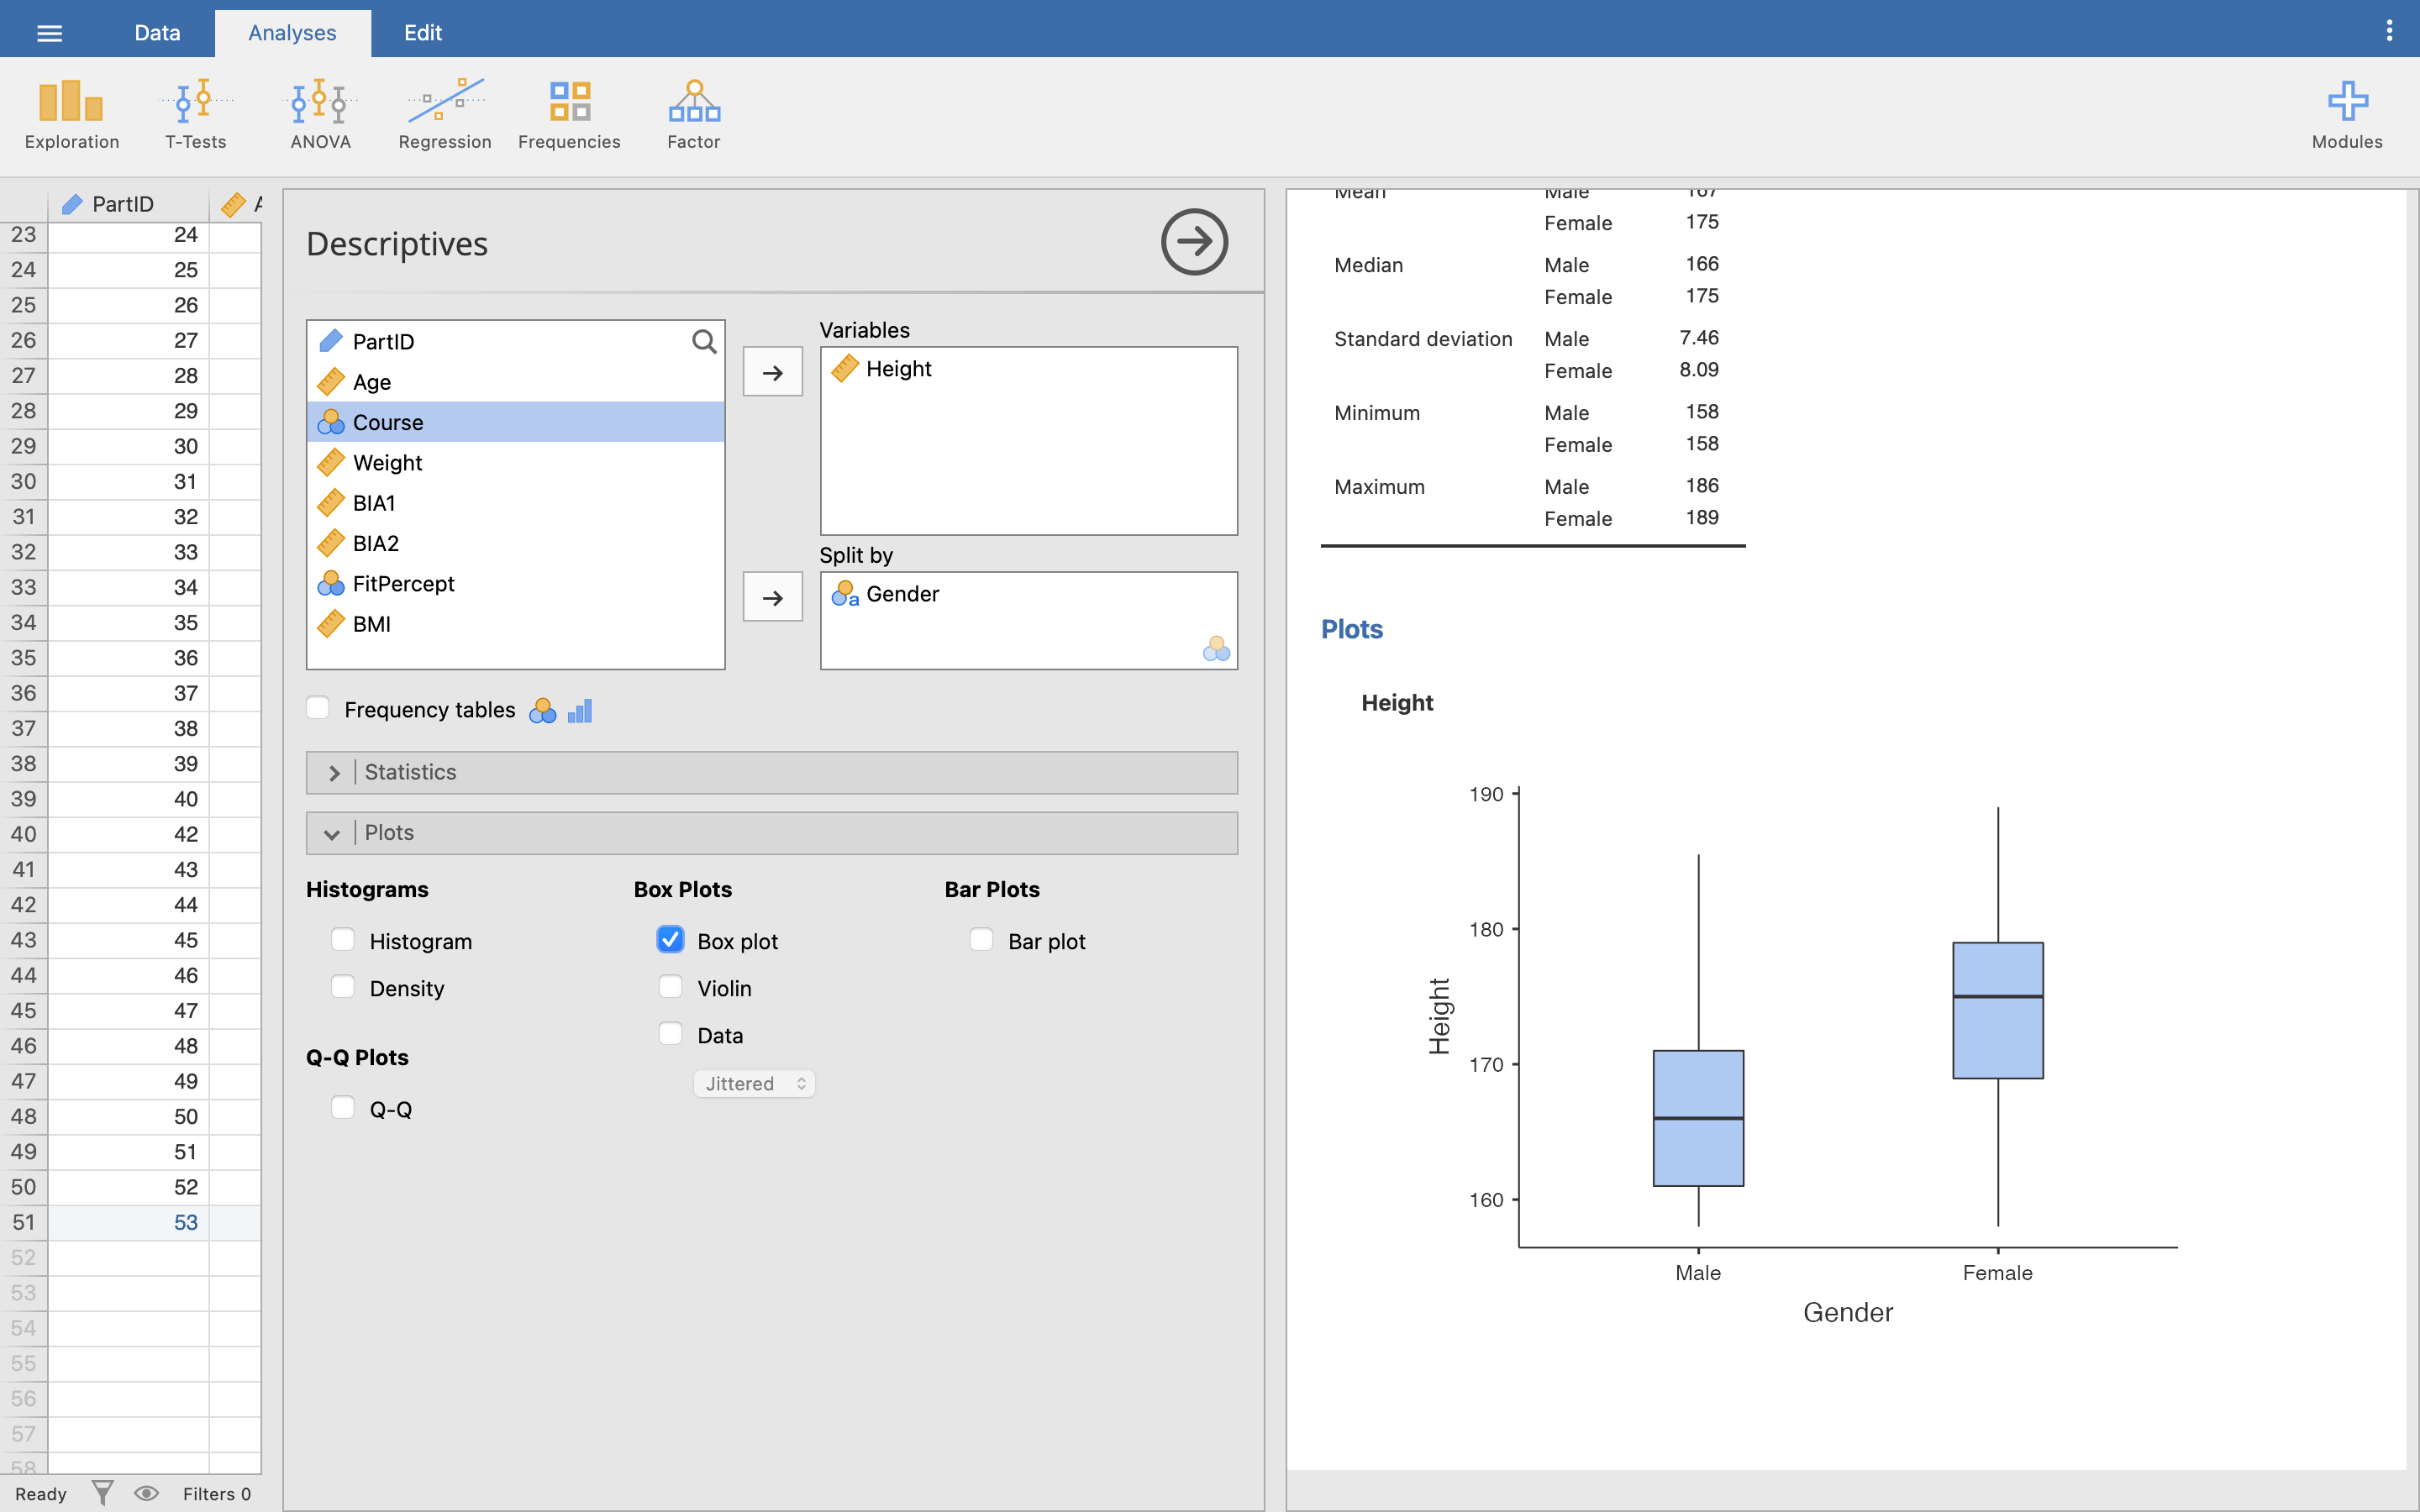
\includegraphics{_imgs/01-18.png}

Remember in a boxplot:

\begin{itemize}
\tightlist
\item
  Top whisker = 1.5 x interquartile range
\item
  Top of box = 3rd quartile
\item
  Line in the middle = median
\item
  Bottom of box = 1st quartile
\item
  Bottom whisker = 1.5 x interquartile range
\end{itemize}

Any outliers are shown with circles beyond the whiskers of the box plot.
There are no recognised outliers in our Height data.

\begin{tcolorbox}[beforeafter skip=1cm, ignore nobreak=true, breakable, colframe=Questions-frame, colback=Questions-bg, coltext=Questions-text, boxsep=2mm, arc=0mm, boxrule=0.5mm]

\protect\hypertarget{Q14}{\protect\hyperlink{A14}{Q14}}. On the boxplot,
what is the approximate value for median male height and median female
height?

\end{tcolorbox}

Feel free to click around now on any other Plot or Statistics options
you think look interesting, and try exploring different variables and
different ways of splitting the data. Remember, if you want to remove
something from the Results viewer, just untick it.

\hypertarget{parametric-testing-and-assumptions}{%
\subsection{Parametric testing and
assumptions}\label{parametric-testing-and-assumptions}}

Before we can decide which test to use we need to look at the `quality'
of our data.

There are 4 assumptions we need to look for:

\begin{itemize}
\tightlist
\item
  Level of data
\item
  Independence of data (often called random allocation of data)
\item
  Normal distribution
\item
  Homogeneity of variance
\end{itemize}

These have all been discussed in the lecture so we will not examine what
they mean here, but we do need to look at the third and fourth
assumptions and test them in Jamovi.

Remember, if you are comparing multiple variables, then you must check
each variable (or segmented variable) against your assumptions.

\hypertarget{tests-of-normality-normal-distribution}{%
\subsubsection{Tests of normality (normal
distribution)}\label{tests-of-normality-normal-distribution}}

While we could simply look at a histogram to visually inspect for a
normal distribution, there are a number of statistical tests we can also
perform. The main statistical test for normality in Jamovi is the
\textbf{Shapiro-Wilk} (SW) test.

Let us examine the distribution of male and female height data. To
compare the two sets of independent data we need to make sure that both
male and female data do not deviate significantly from a normal
distribution. \emph{(Note: testing repeated measures data requires a
slightly different test, but here we will examine normal distribution
for independent samples and look at repeated measures later)}

Still in the Descriptives menu, move \textbf{Height} into the variables
selection, and split the data by \textbf{Gender}. Then, under the
Statistics menu, click the \textbf{Shapiro-Wilk} tick box:

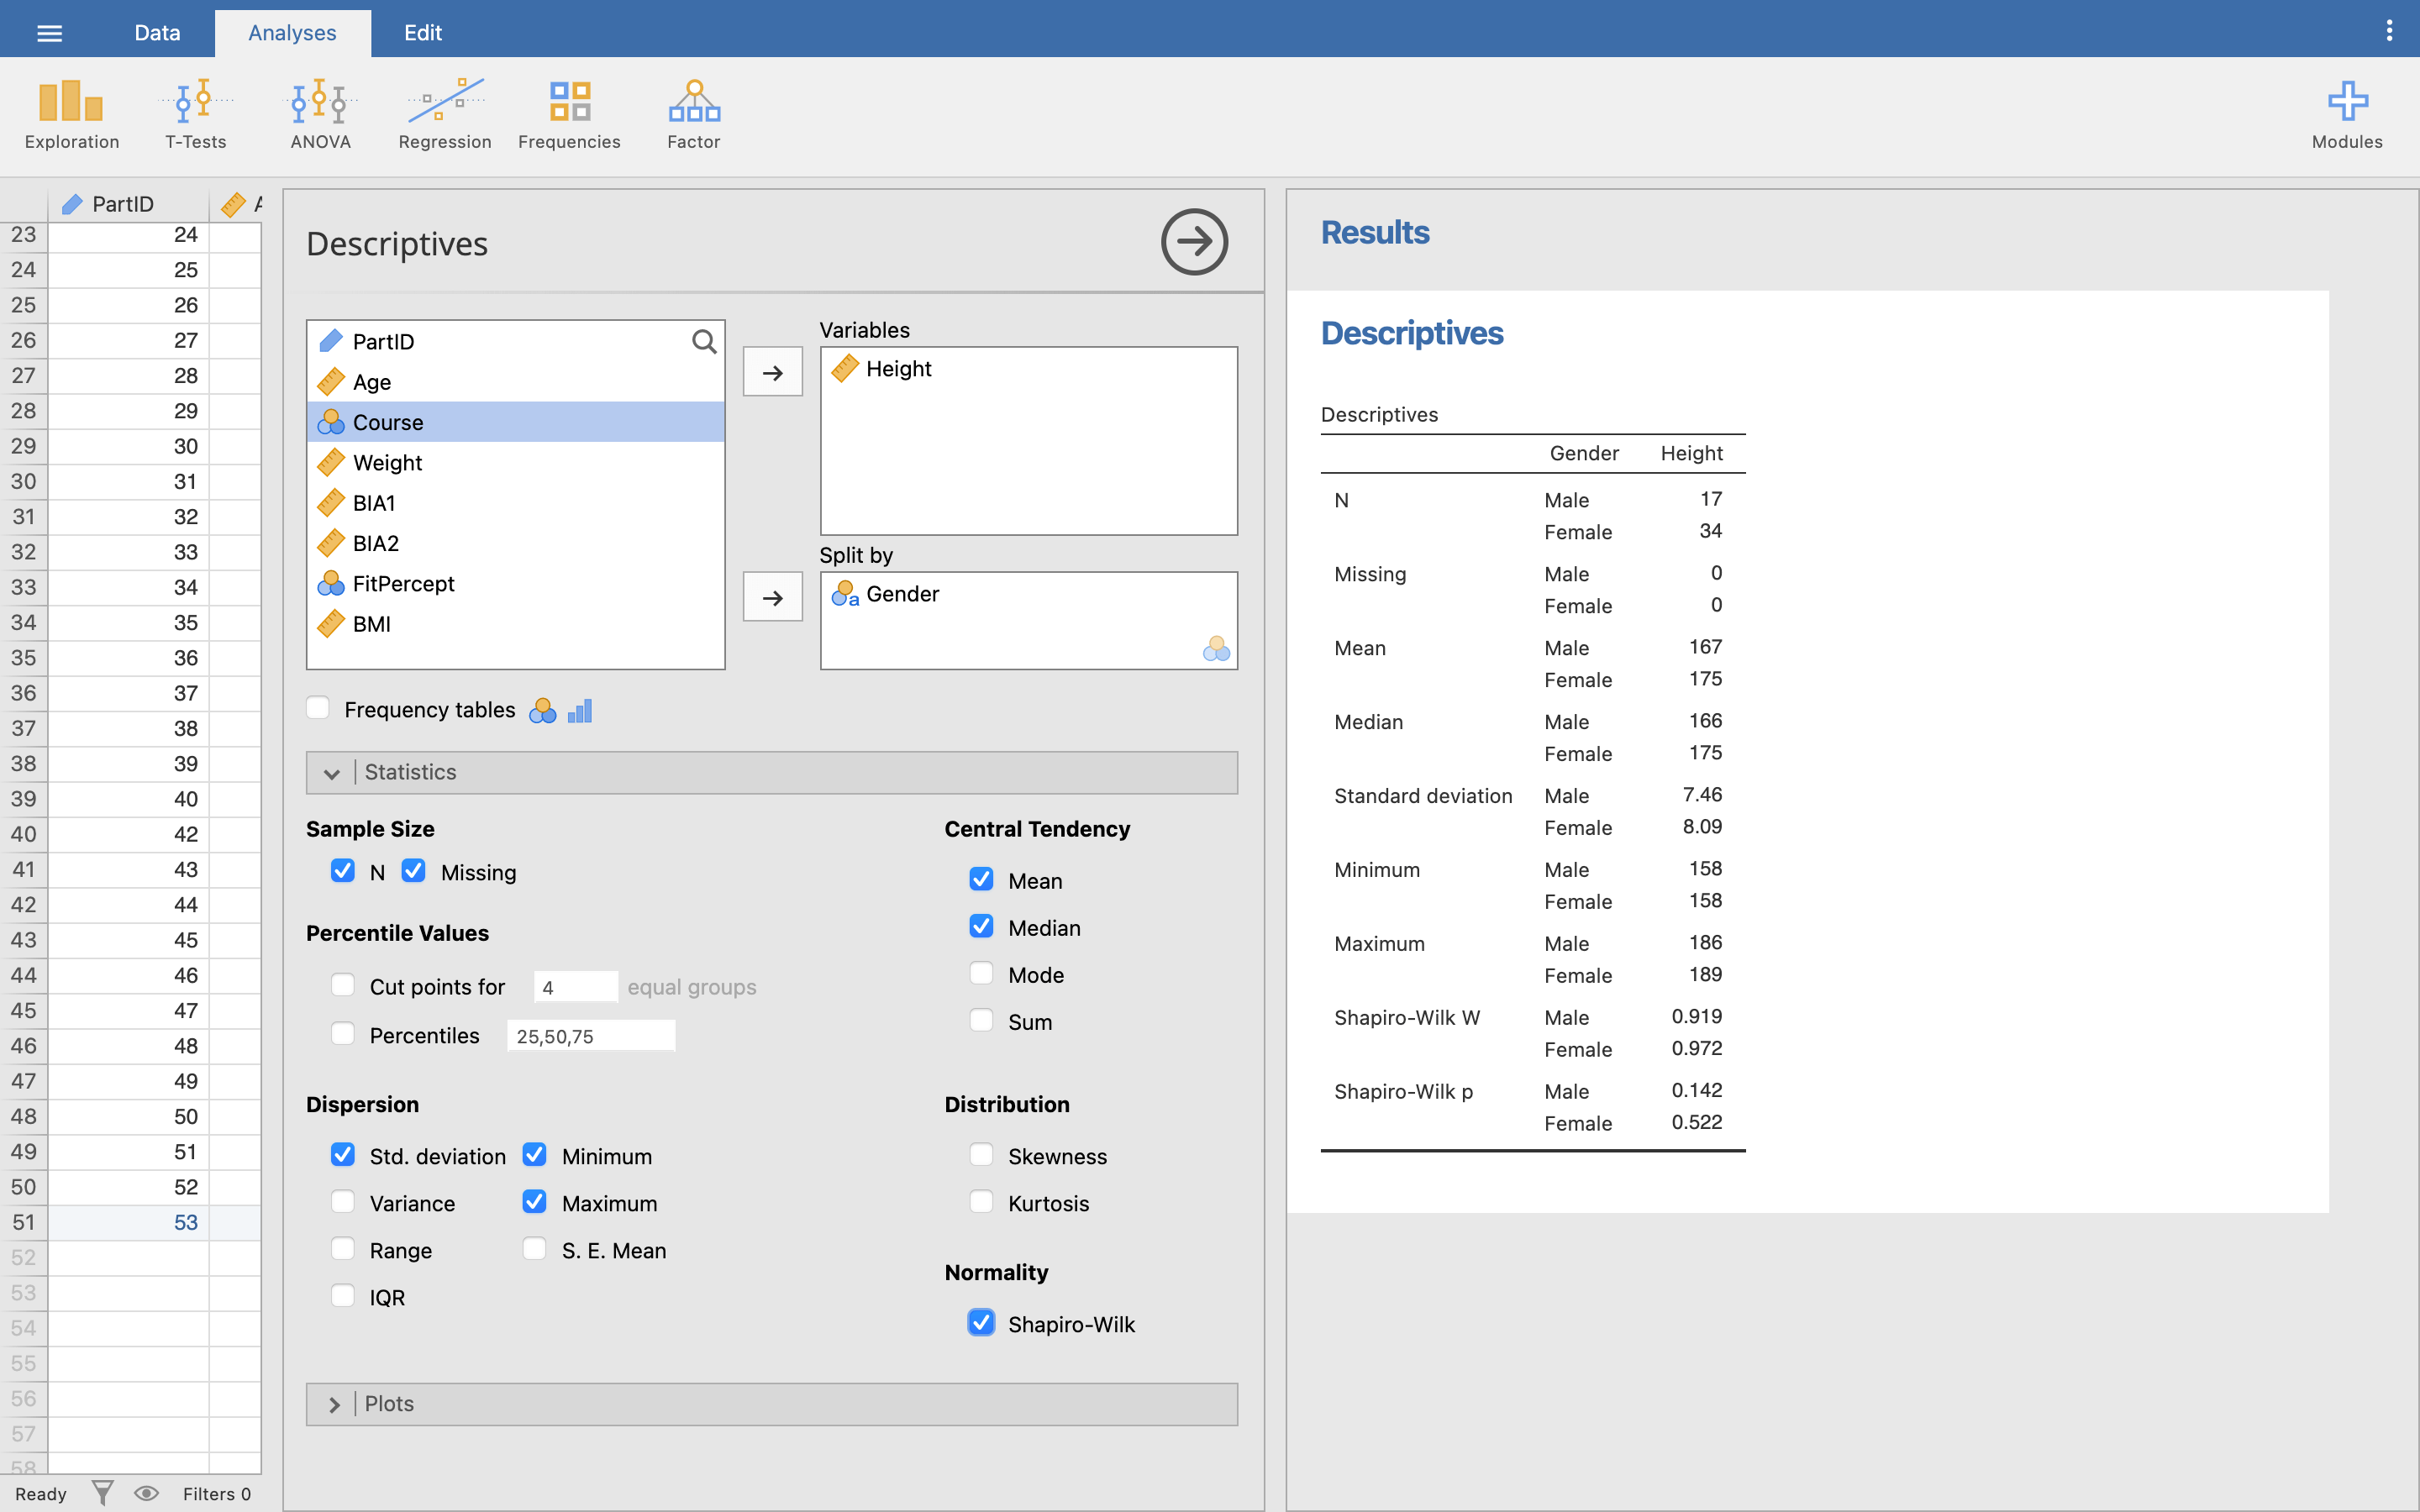
\includegraphics{_imgs/01-19.png}

This will add rows for Shapiro-Wilk \emph{W} and Shapiro-Wilk \emph{p}
values to our descriptives table in the Results viewer.

Here we are testing whether the distribution of Height (by gender) is
normally distributed so we can use parametric tests later. We want to
see whether there is a significant deviation from normality,
i.e.~whether the \emph{p} value result is less than 0.05 for Height for
either Male or Female groups. Both groups have \emph{p} \textgreater{}
0.05. This means there is no significant deviation from a normal
distribution, so the test of normality has been satisfied.

\textbf{Now you try:} Perform a test of normality for \textbf{Weight} by
\textbf{Gender} using the Body Composition.omv data set.

\begin{tcolorbox}[beforeafter skip=1cm, ignore nobreak=true, breakable, colframe=Questions-frame, colback=Questions-bg, coltext=Questions-text, boxsep=2mm, arc=0mm, boxrule=0.5mm]

\protect\hypertarget{Q15}{\protect\hyperlink{A15}{Q15}}. What test would
you run?

\protect\hypertarget{Q16}{\protect\hyperlink{A16}{Q16}}. What p-value
for the test of normality do you get for the Weight data of the Females
group? What does this p-value mean?

\end{tcolorbox}

A simple SW test is ok to start, but you should still perform further
checks on your data. The first two we will examine are \textbf{Skewness}
and \textbf{Kurtosis}.

Still in the Descriptives menu, choose the \textbf{Height} variable
split by \textbf{Gender}. Under Statistics, tick \textbf{Skewness} and
\textbf{Kurtosis}.

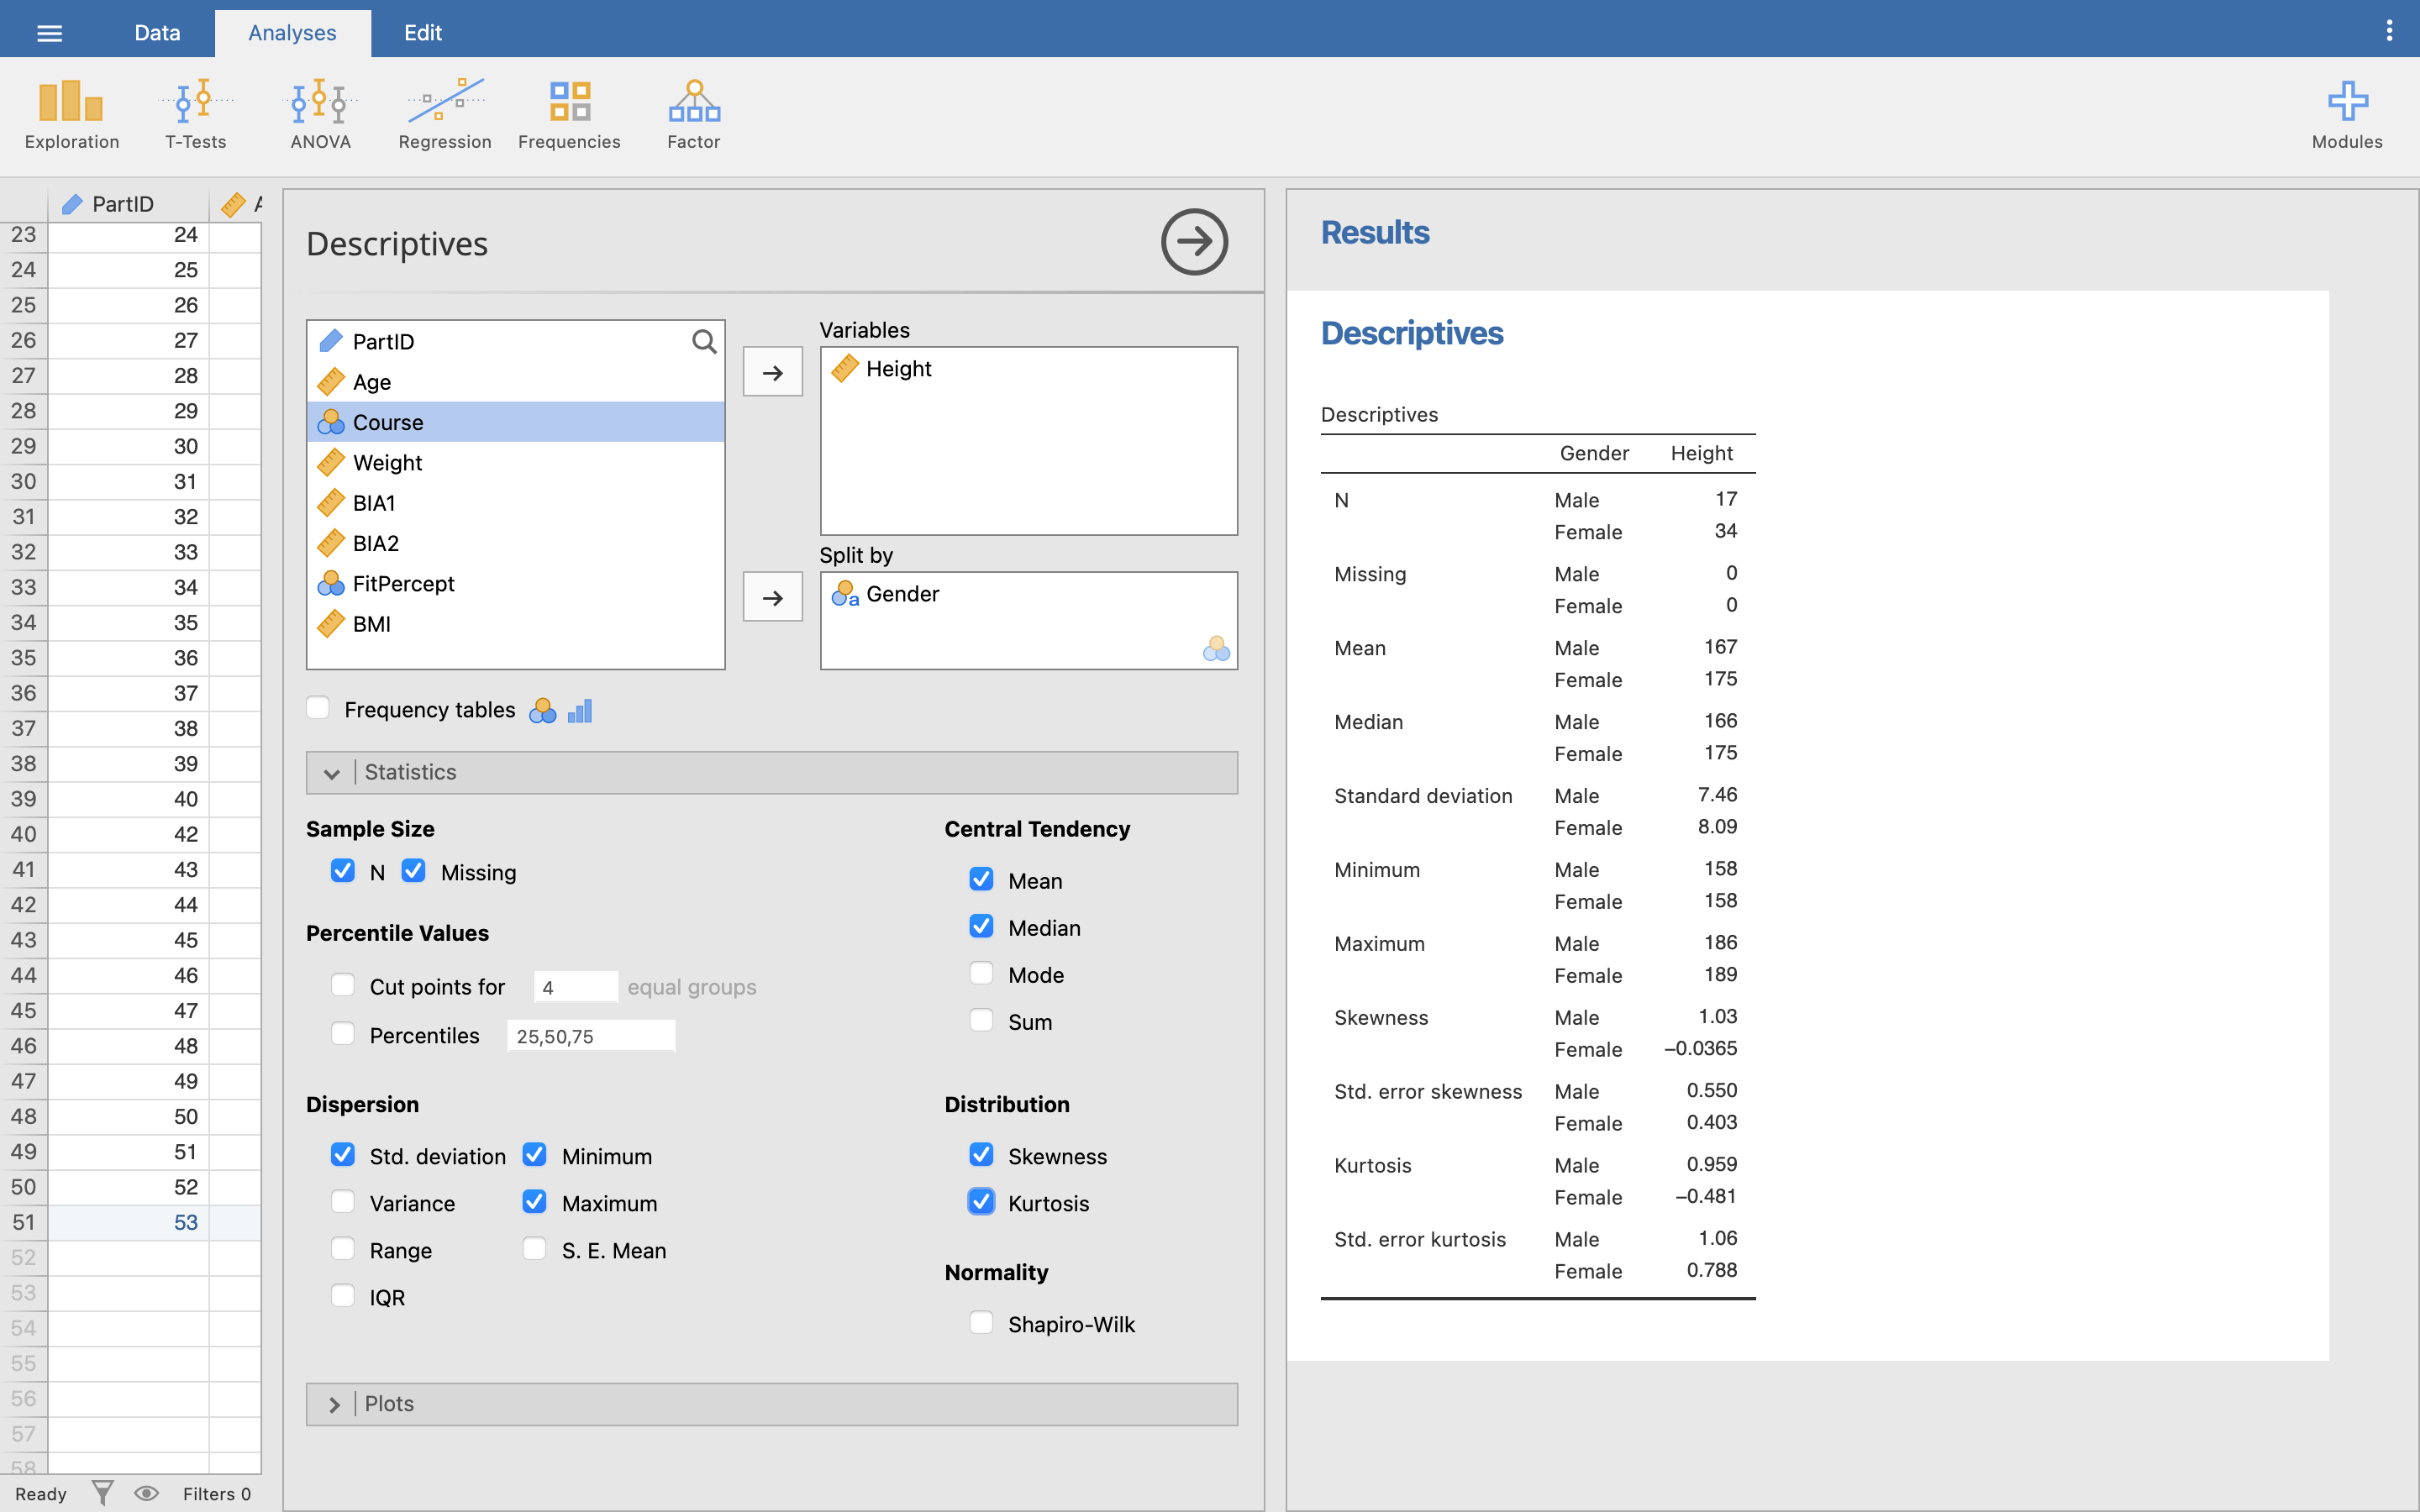
\includegraphics{_imgs/01-20.png}

The first way we can examine this data is to look at the \emph{absolute}
values for Skewness and Kurtosis.

\begin{itemize}
\tightlist
\item
  Male skewness = 1.028
\item
  Male kurtosis = 0.959
\item
  Female skewness = -0.036
\item
  Female kurtosis = -0.481
\end{itemize}

\begin{tcolorbox}[beforeafter skip=1cm, ignore nobreak=true, breakable, colframe=Questions-frame, colback=Questions-bg, coltext=Questions-text, boxsep=2mm, arc=0mm, boxrule=0.5mm]

\protect\hypertarget{Q17}{\protect\hyperlink{A17}{Q17}}. Based on the
raw Skewness and Kurtosis values, describe the shape of your male data
distribution.

\end{tcolorbox}

A rule of thumb suggests that -0.8 to +0.8 is acceptable for skewness
and -3 to +3 is acceptable for kurtosis. Note that the skewness for
males falls outside the -0.8 to 0.8, but all other values are well
within their ranges. Strictly speaking we could suggest that the male
height data is not normally distributed, and has a slight positive skew
(i.e.~a pile up of data on the left hand side).

Turn back on the box plots for this data. You can see the slight
positive skew for the male data with a longer positive tail:

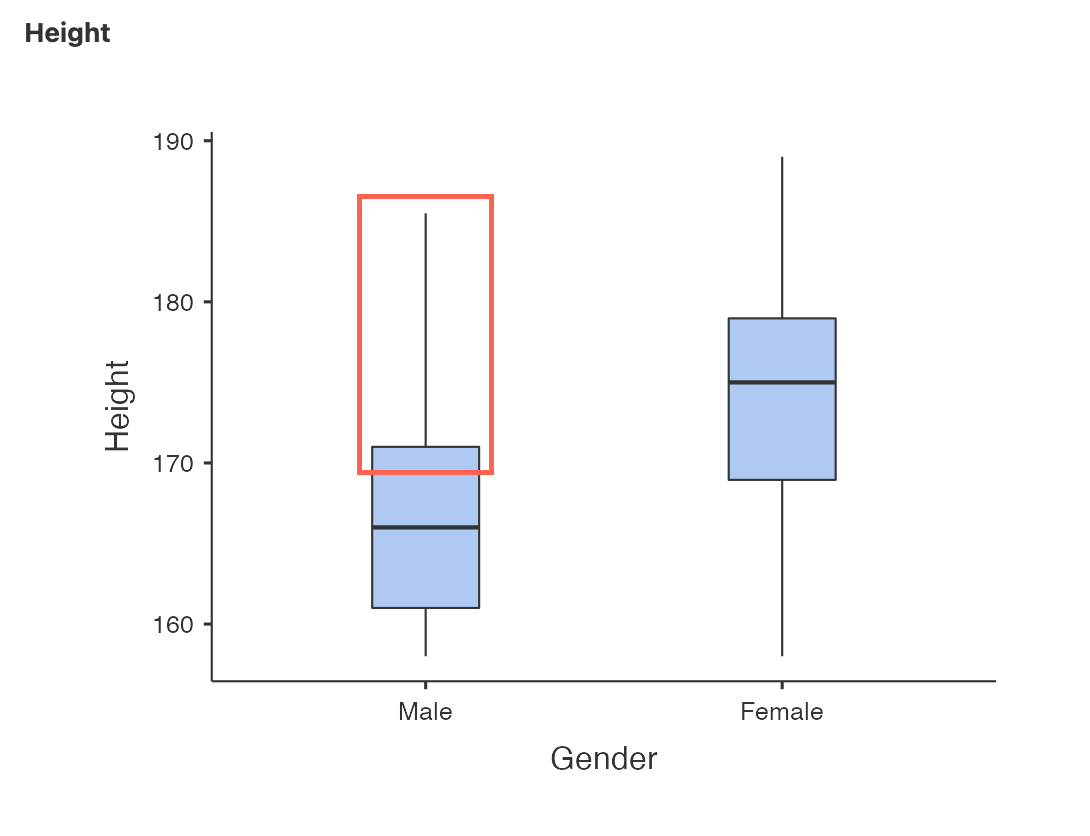
\includegraphics{_imgs/01-21.png}

A further way of examining this data is to convert the height skewness
and kurtosis to a `standardised' value. We do this by taking the value
and dividing it by the \textbf{standard error} of its value. You can
find the standard error values in the Descriptives table just underneath
the Skewness and Kurtosis.

Before we work out our standardised values though, let's change the
number of decimal places Jamovi is using to show our Results, so we can
be more accurate. In the far top right-hand corner of Jamovi is three
white dots - click these to open the \textbf{Preferences} panel. Here,
change the \textbf{Number format} dropdown menu to \textbf{3 dp} (3
decimal places). Click anywhere outside the Preferences panel to close
it again.

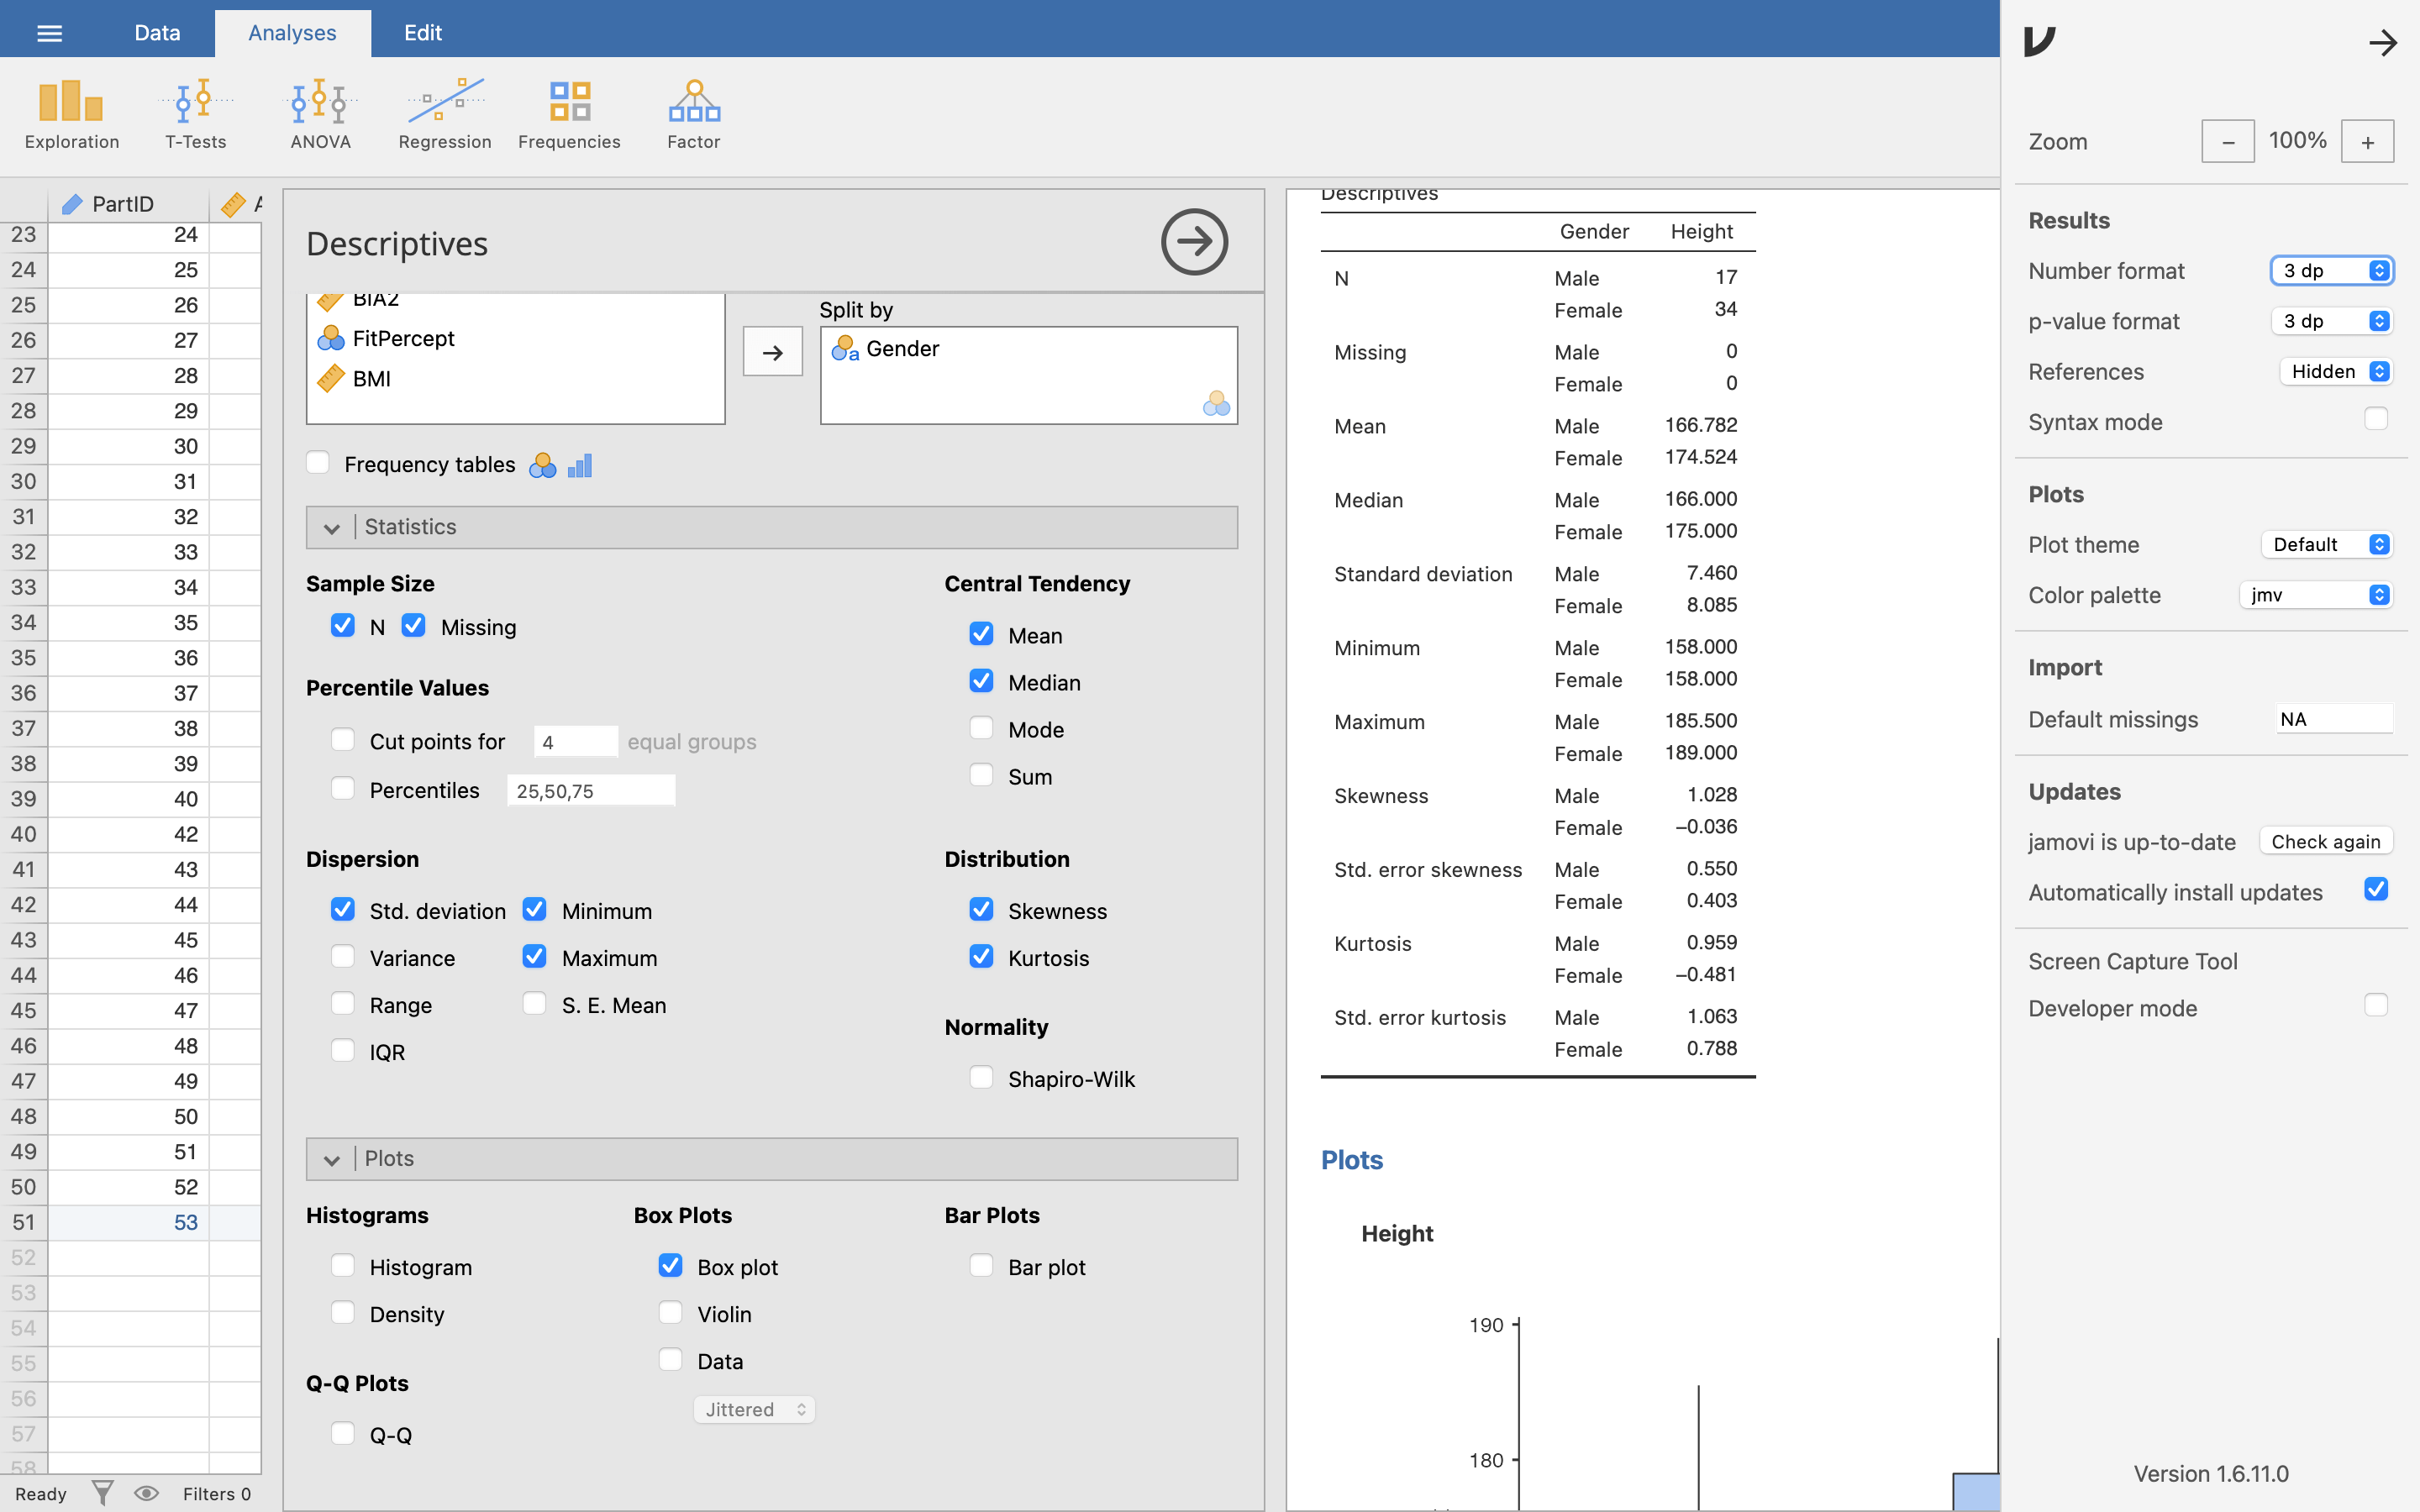
\includegraphics{_imgs/01-22.png}

Now we can calculate our standardised skewness and kurtosis values:

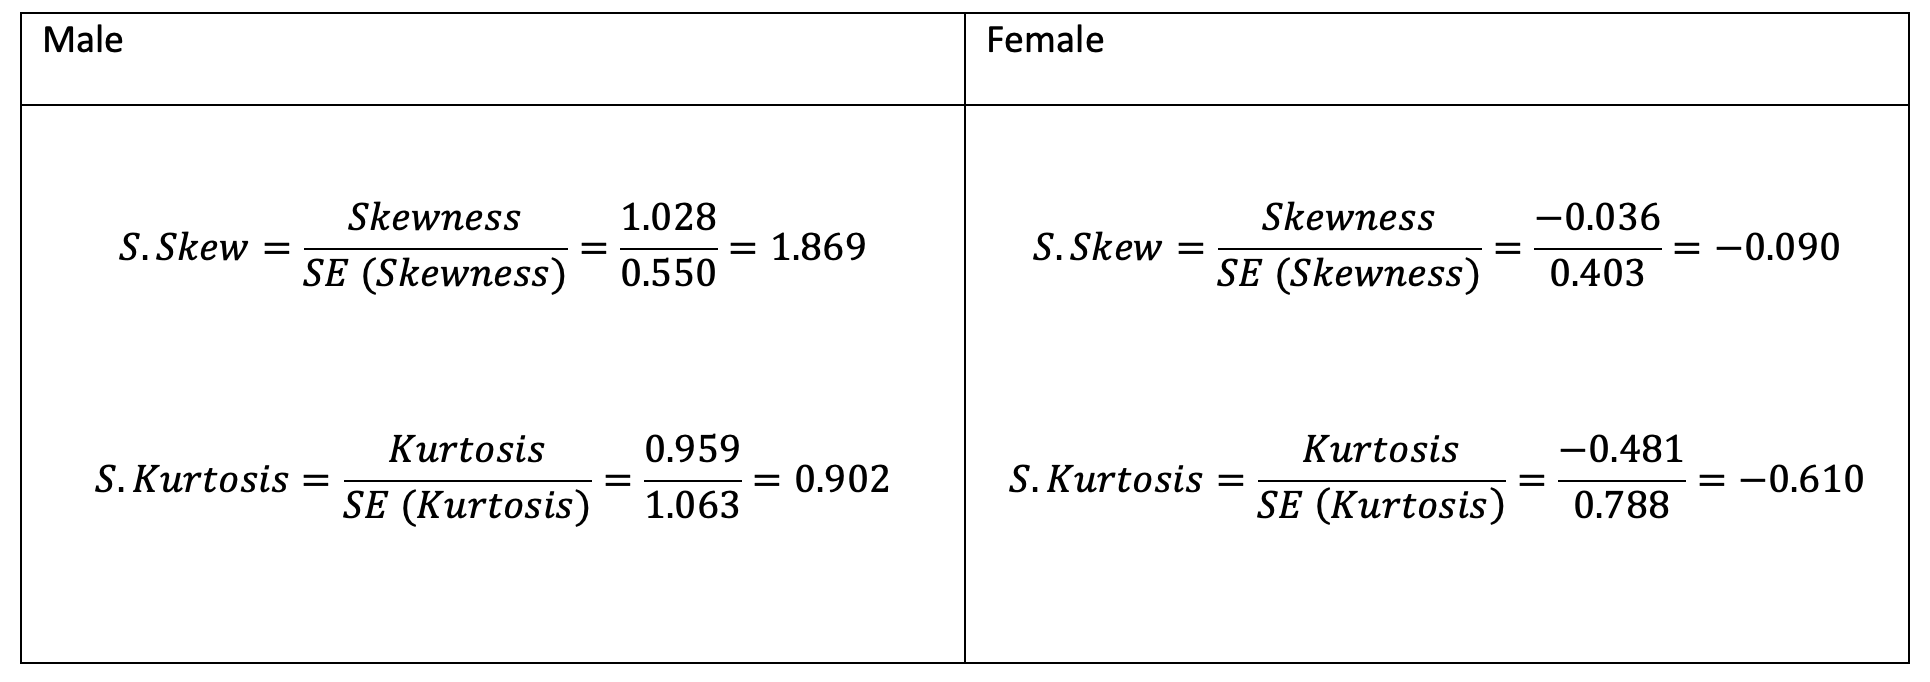
\includegraphics{_imgs/01-23.png}

These values can now be compared to the values we would expect to get by
chance alone, so a value less than -1.96 or greater than 1.96 would
suggest that this distribution is significantly skewed or shows
significant kurtosis. Both of our values are within this range so we can
be happy that our data satisfies the condition of normality.

\begin{tcolorbox}[beforeafter skip=1cm, ignore nobreak=true, breakable, colframe=Aside-frame, colback=Aside-bg, coltext=Aside-text, boxsep=2mm, arc=0mm, boxrule=0.5mm]

\textbf{Note:} You cannot use these tests in very large samples as the
standard skewness and kurtosis values are likely to be significant even
if the skew and kurtosis are only slightly different to normal.

\end{tcolorbox}

Even though we would like to think that statistics should be clear-cut
in giving us answers, you can now see that it can often requires careful
interpretation of your results. Here we have seen two tests that show
our data is normally distributed, with one test that shows it is not!
This is where your experience of working with numbers is going to be
very useful.

\begin{tcolorbox}[beforeafter skip=1cm, ignore nobreak=true, breakable, colframe=Aside-frame, colback=Aside-bg, coltext=Aside-text, boxsep=2mm, arc=0mm, boxrule=0.5mm]

\textbf{Repeated measures normality:} With independent samples data, or
two different groups, you need to check for normality of each separate
group. If you have a repeated measures test, e.g.~your group performs a
test under two different conditions, then rather than testing the
normality of each group, you would test for the normality of the
\emph{difference} between the two conditions.

\end{tcolorbox}

\hypertarget{homogeneity-of-variance}{%
\subsubsection{Homogeneity of variance}\label{homogeneity-of-variance}}

This is a check to see that the samples we are testing come from
populations with a similar variance.

As with the normality test, there is a statistical test and a rule of
thumb. Starting with the rule of thumb, we want to make sure that the
two sample variances differ by a factor of less than 3.

Imagine we wished to compare male and female height - we therefore need
to compare the sample variance of the male height and the female height.

We can view these variances in Jamovi - still with \textbf{Height} split
by \textbf{Gender} selected, tick the \textbf{variance} check box. This
will display the variances for Male and Female groups in our
Descriptives table in the Results viewer.

To test our rule of thumb, take whichever of the two is the larger
variance and divide it by the smaller variance. In our case, that would
be:

\begin{verbatim}
65.368 / 55.649 = 1.17
\end{verbatim}

1.17 is well within our rule of thumb of 3, so we can \emph{assume}
homogeneity of variance. But, let's also test it properly. The
statistical test we will use for this is \textbf{Levene's Test of
Homogeneity}.

To do this, we actually need to go to a new menu option. Click the
right-arrow in the circle at the top right of the Descriptives menu to
close it. Then, still in the \textbf{Analyses} menu, click the
\textbf{T-Tests} icon, and choose \textbf{Independent Samples T-Test}
from the dropdown menu.

This will open the \textbf{T-Test} menu. You'll see that it looks very
similar to the Descriptives menu - we choose our variables of interest
and how we want to split them (here called \textbf{Grouping Variable})
at the top, and just tick the things we want Jamovi to show us
underneath.

Move \textbf{Height} into our variables selection and split by
\textbf{Gender} again. Don't worry about any of the other options, but
just tick the \textbf{Homogeneity test} option under
\textbf{Assumptions}.

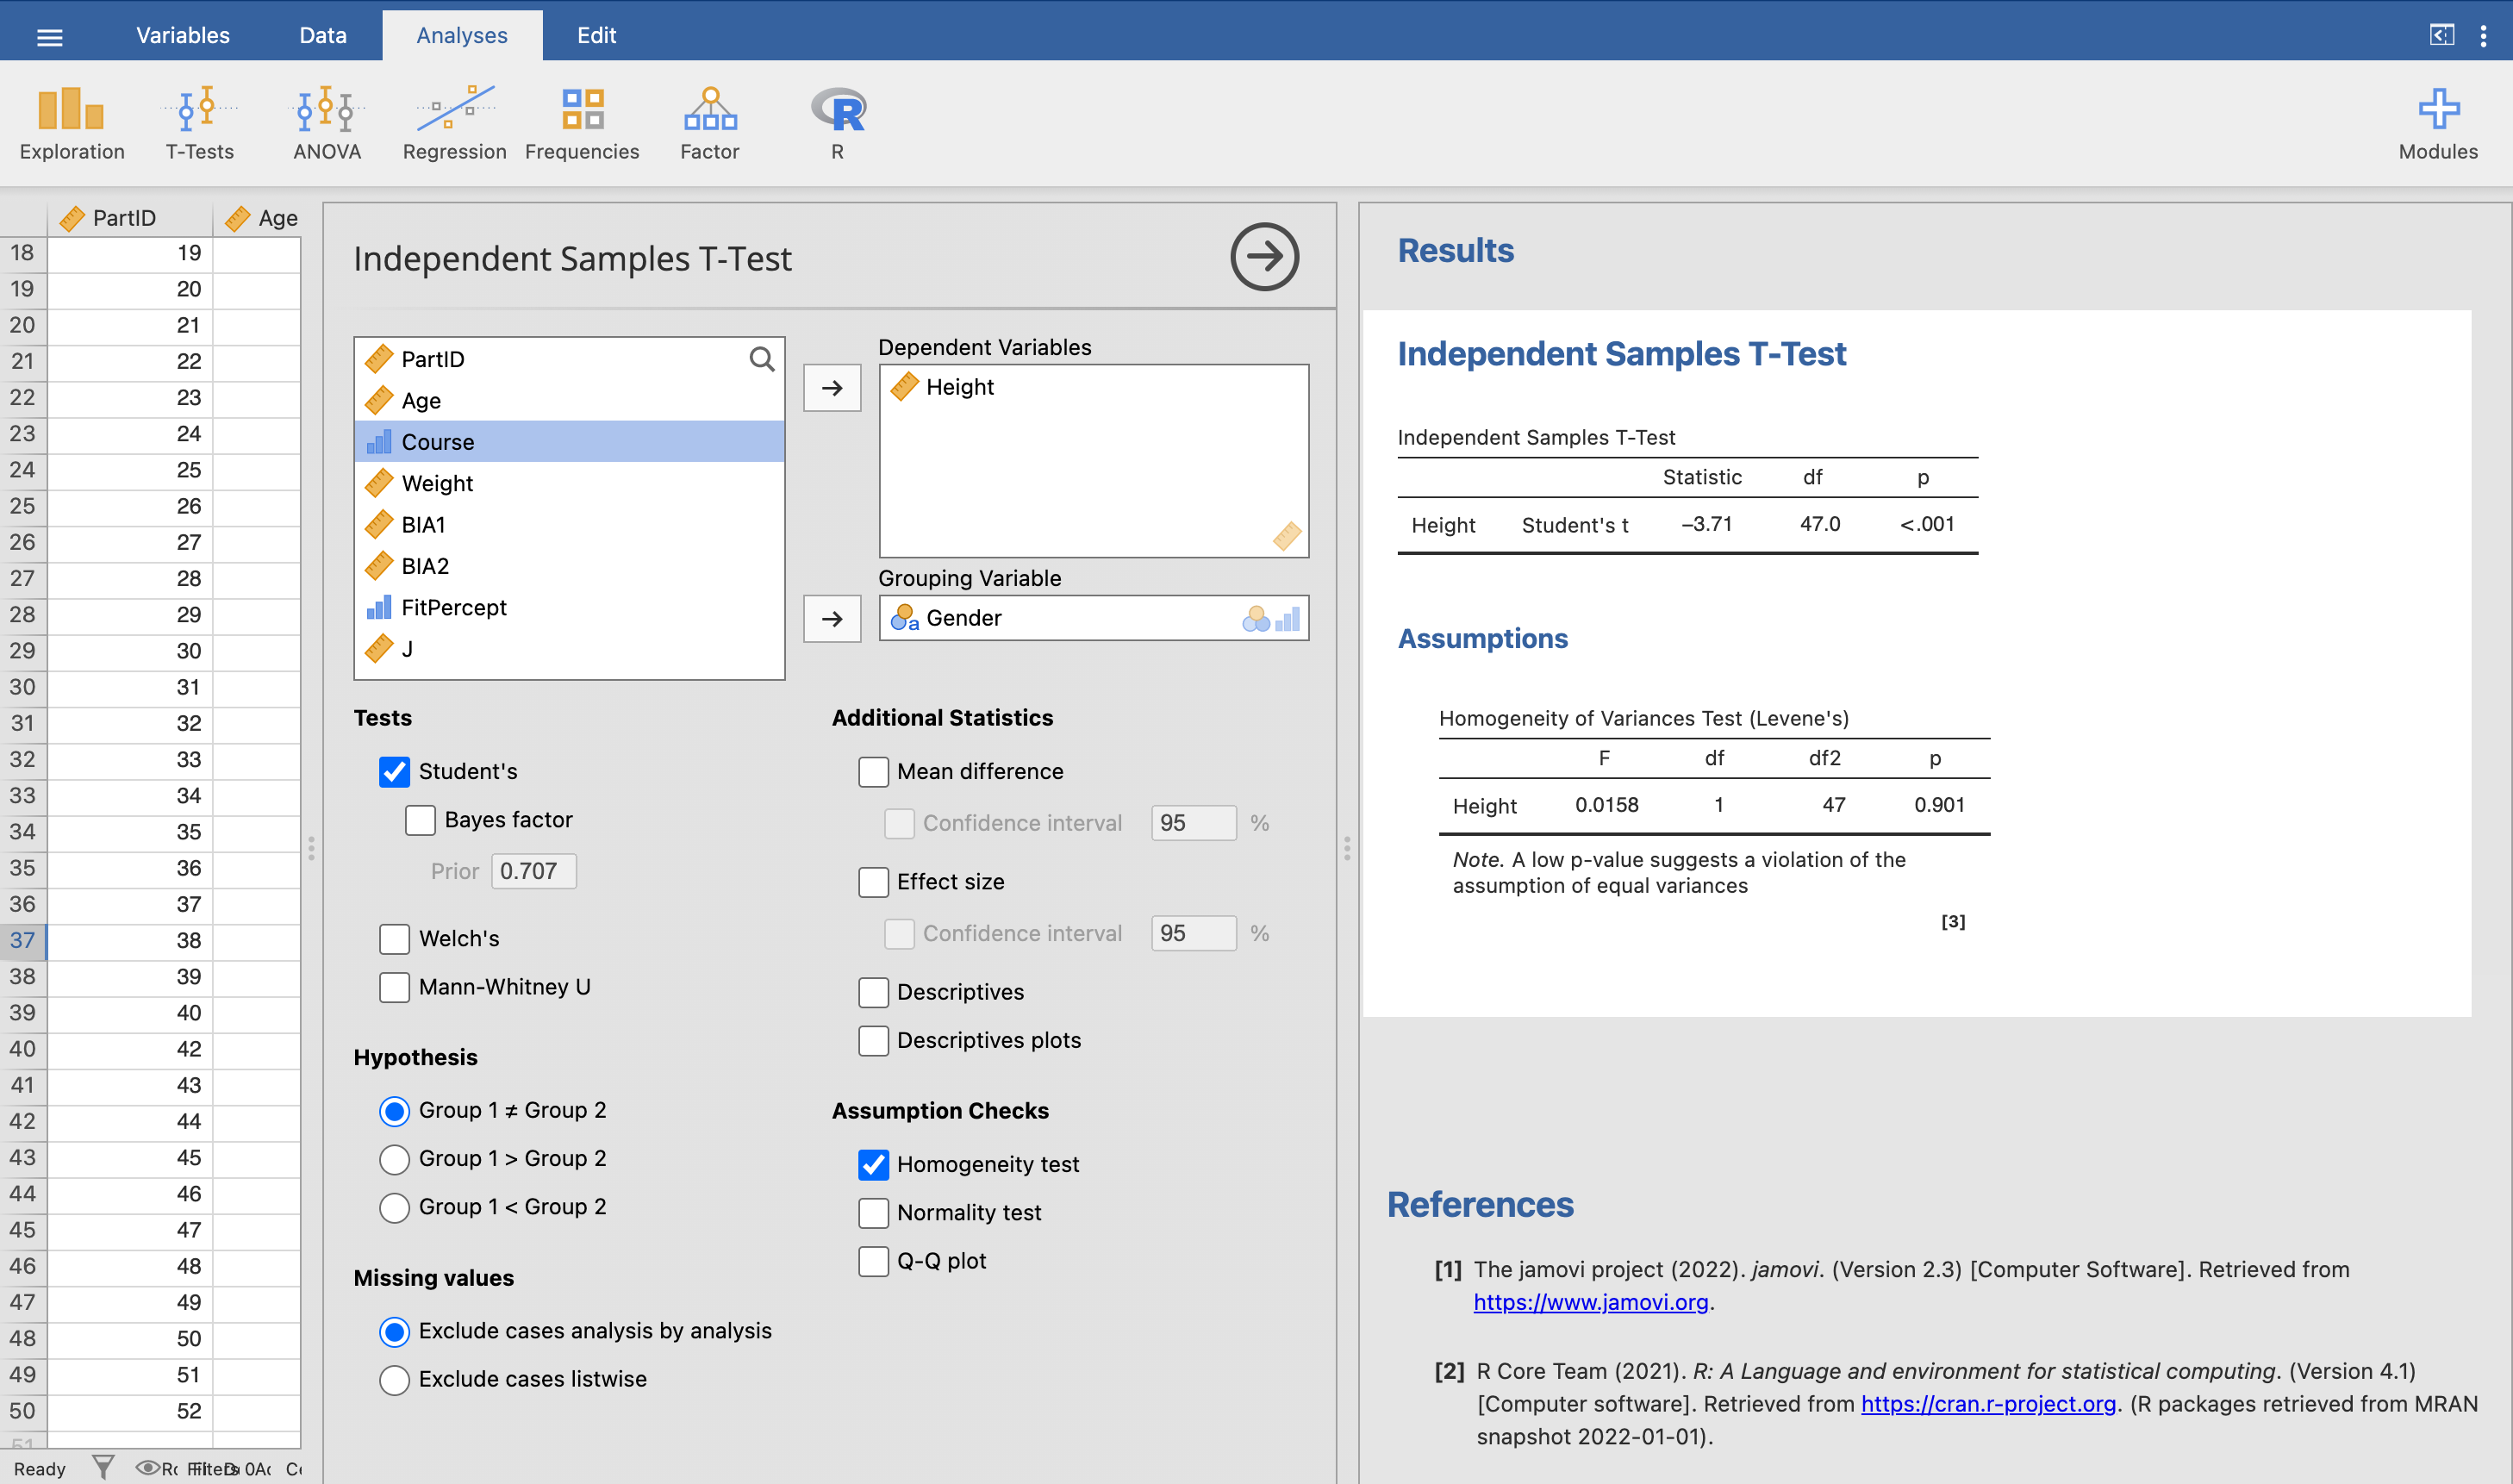
\includegraphics{_imgs/01-24.png}

Notice how this gives us a new area in the Results viewer, under the
heading \textbf{Independent Samples T-Test}. But, our Descriptives table
is still displayed above it (you might need to scroll back up). If you
click on the descriptives table in the Results, the descriptive menu
will open back up in the middle, and you can make any changes. This is
how your results are stored and edited in Jamovi - just click them in
the viewer to open the menu for that particular result. If you want to
remove a result from your viewer entirely, right-click on it's title and
select `Remove' from the pop-up menu.

We won't worry about the T-Test results for now - just look at the table
titled \textbf{Homogeneity of Variances Test (Levene's)}. Here, we are
looking to see if the test result is significant, just as we did for the
normality test. The non-significant value of \emph{p} = 0.675 says that
the variances are not significantly different to each other and we can
continue with our parametric tests.

\textbf{Now you try:} Repeat the test of Homogeneity of Variance for
Weight by Gender.

\begin{tcolorbox}[beforeafter skip=1cm, ignore nobreak=true, breakable, colframe=Questions-frame, colback=Questions-bg, coltext=Questions-text, boxsep=2mm, arc=0mm, boxrule=0.5mm]

\protect\hypertarget{Q18}{\protect\hyperlink{A18}{Q18}}. What is the
Levene statistic and \emph{p} value, and what does this mean?

\protect\hypertarget{Q19}{\protect\hyperlink{A19}{Q19}}. Would you be
happy running a parametric test on this data? And why?

\end{tcolorbox}

\newpage{}

\hypertarget{antwoorden-op-vragen}{%
\section{Antwoorden op vragen}\label{antwoorden-op-vragen}}

\begin{tcolorbox}[beforeafter skip=1cm, ignore nobreak=true, breakable, colframe=Questions-frame, colback=Questions-bg, coltext=Questions-text, boxsep=2mm, arc=0mm, boxrule=0.5mm]

\protect\hypertarget{A1}{\protect\hyperlink{Q1}{A1}}. In dit
gegevensbestand staan 9 kolommen met gegevens: deelnemer ID, leeftijd,
geslacht, cursus, gewicht, lengte, BIA1, BIA2 en FitPercept.

\protect\hypertarget{A2}{\protect\hyperlink{Q2}{A2}}. Er zijn 50 rijen
met gegevens, oftewel 50 `cases' (eenheden). Gebruik PartId niet om het
aantal records weer te geven.

\protect\hypertarget{A3}{\protect\hyperlink{Q3}{A3}}. Ook al is er een
rijnummer, dit identificeert geen specifieke eenheid uit de gegevens,
alleen de volgorde van de rijen (of cases) die momenteel worden
weergegeven. Met de PartId kan de gebruiker gemakkelijk een bepaalde
case identificeren. Als je de gegevens sorteert of filtert, kunnen de
rijnummers veranderen, maar PartId blijft consistent.

\protect\hypertarget{A4}{\protect\hyperlink{Q4}{A4}}. Ten eerste zal de
PartId uniek zijn, maar het maakt het ook mogelijk om de gegevens te
anonimiseren.

\protect\hypertarget{A5}{\protect\hyperlink{Q5}{A5}}. Jamovi heeft vier
hoofdtypen gegevens: Nominaal, Ordinaal, Continu en ID. Continu is een
combinatie van de gegevenstypen Interval en Ratio. ID is een uniek
gegevenstype voor Jamovi, dat alleen wordt gebruikt voor
deelnemers-ID-variabelen, dat vergelijkbaar is met een nominaal
gegevenstype, maar zonder categorieniveaus of labels.

\protect\hypertarget{A6}{\protect\hyperlink{Q6}{A6}}. Het veld is puur
een `naam' voor elk record, je kunt er niet uit afleiden dat er een
volgorde is, of dat het ene voor of na het andere moet komen.

\protect\hypertarget{A7}{\protect\hyperlink{Q7}{A7}}. Vrouwen zijn
gemiddeld zwaarder. Gemiddelde massa vrouw = 76.855 kg, gemiddelde massa
man = 64.153 kg.

\protect\hypertarget{A8}{\protect\hyperlink{Q8}{A8}}. Er zijn 17 mannen
en 33 vrouwen in de steekproef.

\protect\hypertarget{A9}{\protect\hyperlink{Q9}{A9}}. Het is moeilijk
definitief te zeggen of de machines `hetzelfde' laten zien. De
beschrijvende informatie zou suggereren dat de waarden `gemiddeld'
hetzelfde zijn, maar afzonderlijke machines binnen de steekproef zouden
heel verschillende resultaten kunnen laten zien, bijv. machine 1 geeft
15\% en 25\% voor twee deelnemers, maar machine 2 geeft 25\% en 15\%
voor dezelfde twee. Gemiddeld' zouden beide machines 20\% aangeven. Het
feit dat getallen op elkaar `lijken' betekent niet dat ze statistisch
gezien hetzelfde zijn.

\protect\hypertarget{A10}{\protect\hyperlink{Q10}{A10}}. 50 studenten
hebben een cursus opgegeven.

\protect\hypertarget{A11}{\protect\hyperlink{Q11}{A11}}. Sporttherapie,
met 54\%.

\protect\hypertarget{A12}{\protect\hyperlink{Q12}{A12}}. 16\% van de
studenten volgt Sport- en Danstherapie.

\protect\hypertarget{A13}{\protect\hyperlink{Q13}{A13}}. Uit de grafiek
blijkt dat vrouwen variabeler zijn en zich links en rechts van de mannen
in de grafiek uitstrekken. De standaarddeviatie is ook groter voor
vrouwen (18,08 kg) vergeleken met mannen (13,84 kg).

\protect\hypertarget{A14}{\protect\hyperlink{Q14}{A14}}. In de boxplot
is de mediaan de dikke zwarte lijn in het midden van elk vak. De
geschatte waarde voor de mediane lengte bij mannen is 166 cm en bij
vrouwen 175 cm.

\protect\hypertarget{A15}{\protect\hyperlink{Q15}{A15}}. Voor een
normaliteitstest zou je de Shapiro-Wilk test uitvoeren.

\protect\hypertarget{A16}{\protect\hyperlink{Q16}{A16}}. Voor vrouwen is
Shapiro-Wilk \emph{p} = 0,291. Dit is vergelijkbaar met de
\emph{p}-waarde voor mannen. Een niet-significante waarde suggereert dat
de steekproefverdeling voor het gewicht van vrouwen niet significant
verschilt van een normale verdeling, zodat aan een van de aannames voor
het uitvoeren van parametrische tests is voldaan.

\protect\hypertarget{A17}{\protect\hyperlink{Q17}{A17}}. De positieve
scheefheidswaarde (1,028) suggereert dat de grafiek een iets langere
rechterstaart heeft, en de positieve kurtosiswaarde (0,959) suggereert
dat de curve iets dunner is dan een normale verdeling (ook wel
leptokurtisch genoemd).

\protect\hypertarget{A18}{\protect\hyperlink{Q18}{A18}}. De Levene
teststatistiek, F = 0,642, p = 0,427 (gebaseerd op het gemiddelde). Dit
betekent dat de varianties niet significant verschillen, dus we kunnen
homogeniteit van variantie aannemen.

\protect\hypertarget{A19}{\protect\hyperlink{Q19}{A19}}. Ja, we hebben
voldaan aan de vier voorwaarden, 1. Het zijn gegevens van hoog
meetniveau, 2. Ze zijn willekeurig toegewezen/selecteerd, 3. Ze zijn
normaal verdeeld, en 4. De varianties zijn gelijk.

\end{tcolorbox}



\end{document}
